% \AtBeginDocument{%
%   \pdfhorigin=1sp
%   \pdfvorigin=1sp
%   \paperwidth=297truemm
%   \paperheight=210truemm
% }

\documentclass{article}

\usepackage{url}
\usepackage{multicol}
\usepackage{tabularx}
% \usepackage{sem-a4}
\usepackage[OT1]{fontenc}
\usepackage{alltt}
\usepackage{graphicx}
%\usepackage{color}
\usepackage{fancyhdr} % Required for custom headers
\usepackage{listings} % Required for insertion of code
\usepackage{extramarks} % Required for headers and footers
\usepackage[usenames,dvipsnames]{color} % Required for custom colors
\usepackage{courier} % Required for the courier font
\usepackage{lastpage} % Required to determine the last page for the footer
\usepackage[tikz]{bclogo}
\usepackage{mdframed} % for frames around tasks

% Margins
\topmargin=-0.45in
\evensidemargin=0in
\oddsidemargin=0in
\textwidth=6.5in
\textheight=9.0in
\headsep=0.25in

\linespread{1.1} % Line spacing

% Set up the header and footer
\pagestyle{fancy}
\lhead{\hmwkAuthorName} % Top left header
\chead{\hmwkClass\ (\hmwkTitle)} % Top center head
\rhead{\firstxmark} % Top right header
\lfoot{\lastxmark} % Bottom left footer
\cfoot{} % Bottom center footer
\rfoot{Page\ \thepage\ of\ \protect\pageref{LastPage}} % Bottom right footer
\renewcommand\headrulewidth{0.4pt} % Size of the header rule
\renewcommand\footrulewidth{0.4pt} % Size of the footer rule

\setlength\parindent{0pt} % Removes all indentation from paragraphs

%------------------------------------------------------------------------------
%	CODE INCLUSION CONFIGURATION
%------------------------------------------------------------------------------

\definecolor{MyDarkGreen}{rgb}{0.0,0.4,0.0} % This is the color used for comments
\lstloadlanguages{C}
\lstset{language=C, % Use C
        frame=single, % Single frame around code
        basicstyle=\small\ttfamily, % Use small true type font
        keywordstyle=[1]\color{Blue}\bf, % functions bold and blue
        keywordstyle=[2]\color{Purple}, % function arguments purple
        keywordstyle=[3]\color{Blue}\underbar, % Custom functions underlined and blue
        identifierstyle=, % Nothing special about identifiers                                         
        commentstyle=\usefont{T1}{pcr}{m}{sl}\color{MyDarkGreen}\small, % Comments small dark green courier font
        stringstyle=\color{Purple}, % Strings are purple
        showstringspaces=false, % Don't put marks in string spaces
        tabsize=4, % 4 spaces per tab
        %
        % Put standard Perl functions not included in the default language here
        morekeywords={rand},
        %
        % Put Perl function parameters here
        morekeywords=[2]{on, off, interp},
        %
        % Put user defined functions here
        morekeywords=[3]{test},
       	%
        morecomment=[l][\color{Blue}]{...}, % Line continuation (...) like blue comment
        numbers=left, % Line numbers on left
        firstnumber=1, % Line numbers start with line 1
        numberstyle=\tiny\color{Blue}, % Line numbers are blue and small
        stepnumber=5 % Line numbers go in steps of 5
}

% Creates a new command to include a C code file
%   arg1: filename of the script (without .c)
%   arg2: caption
\newcommand{\ccode}[2]{
\begin{itemize}
\item[]\lstinputlisting[caption=#2,label=#1]{#1.c}
\end{itemize}
}

%------------------------------------------------------------------------------
%	NAME AND CLASS SECTION
%------------------------------------------------------------------------------

\newcommand{\hmwkTitle}{Advanced Unix programming} % Assignment title
\newcommand{\hmwkDueDate}{Monday,\ January\ 1,\ 2012} % Due date
\newcommand{\hmwkClass}{NSWI\ 0138} % Course/class
\newcommand{\hmwkClassTime}{10:30am} % Class/lecture time
\newcommand{\hmwkClassInstructor}{Kotal} % Teacher/lecturer
\newcommand{\hmwkAuthorName}{Vladim\'{i}r Kotal} % Your name

%------------------------------------------------------------------------------
% colored boxes
%------------------------------------------------------------------------------

% Info
%  arg1: caption
%  arg2: content
\newcommand{\infoBox}[2]{
\begin{bclogo}[logo=\bcinfo,arrondi=.3,couleur=green!20,marge=10]{#1}
#2
\end{bclogo}
}

% Alert
%  arg1: caption
%  arg2: content
\newcommand{\alertBox}[2]{
\begin{bclogo}[logo=\bcattention,arrondi=.3,couleur=red!20,marge=10]{#1}
#2
\end{bclogo}
}

% -----------------------------------------------------------------------------
% various
% -----------------------------------------------------------------------------

% Might seem really stupid but my LaTeX installation does not allow to use word
% "unix". It replaces it with an empty string. So, we must use a workaround.
\def\myun{un}
\def\myix{ix}

\usepackage{color}
\definecolor{MyDarkBlue}{rgb}{0.11,0.14,0.56}
\definecolor{MyDarkGreen}{rgb}{0.00,0.74,0.00}

% hyperref docs:
%   http://www.tug.org/applications/hyperref/manual.html
%   http://en.wikibooks.org/wiki/LaTeX/Hyperlinks
%
%\usepackage[plainpages=false,colorlinks,linkcolor=MyDarkBlue,citecolor=MyDarkGreen,dvipdfm]{hyperref}
% NOTE: use pdfborder to create box around the links (colorlinks option would
%       reset it to produce no border)
\usepackage[bookmarks,breaklinks=true,colorlinks=false,%
pdfauthor={Vladimir Kotal \& Jan Pechanec},%
pdftitle={Advanced Unix Programming},%
pdfsubject={Slides for the Advanced Unix Programming course (NSWI138)},%
pdfkeywords={Unix, programming, advanced, lecture, MFF, MFF-UK},%
pagebackref=true,%
]{hyperref}

% by default \url will use monospaced font. suppress this and use normal font.
\urlstyle{same}

\chardef\clqq=254  \sfcode254=0 \lccode254=0
\chardef\crqq=255  \sfcode255=0 \lccode255=0
\DeclareRobustCommand\uv[1]{{\leavevmode{},,#1''}}

\setlength{\textwidth}{0.9\textwidth}

% bold
\newcommand{\emsl}[1]{\textbf{#1}} % Emphasizing

\newcommand{\emprg}[1]{\emph{\color[rgb]{1,0,0} #1}} % Emphasize in programs
\newcommand{\emblue}[1]{\emph{\color[rgb]{0,0,1} #1}} % emph in blue

% my very important note
\newcommand{\rednote}[1]{\color[rgb]{1,0,0} #1}

\newcommand{\CHECK}[1]{{\color[rgb]{1,0,0} $\star$#1$\star$}} % What should be
							      % checked
\newenvironment{itemize2} % Itemize with smaller font
    {\begin{itemize}\small} {\end{itemize}}
    
\newsavebox{\boxTMP}
\newcommand{\raisetab}[1]{ % Align first table row with other text
    \sbox{\boxTMP}{\begin{tabular}{c}\hline X\\\hline\end{tabular}}
    \raisebox{\ht\boxTMP}{#1}}

\newcommand{\funnm}[1] {% Emphasized function name
    {\bf #1}}

\newcommand{\funml}[1] { % Multi-line function prototype
    \begin{minipage}{\slidewidth}
    \vspace{-1ex}\texttt{\begin{tabbing}#1\end{tabbing}}
    \end{minipage}}

\newcommand{\bs}{\char92\relax} % TT backslash

\newtoks\prgcharsI\newtoks\prgcharsII
{\catcode`\_=13\catcode`\&=13\global\prgcharsI={_}\global\prgcharsII={&}}
\def\prgchars{ % Do not require backslashes for these characters often used
                % in C program source code
    \catcode`\_=13\catcode`\&=13
    \expandafter\def\the\prgcharsI{\_}\expandafter\def\the\prgcharsII{\&}}


%
% colored frame around source code path to examples
% which is actually a link
%
\newcommand{\priklad}[1]{\fcolorbox{cyan}{white}{%
  \href{http://mff.devnull.cz/pvu2/src/#1}{\texttt{#1}}}}

%------------------------------------------------------------------------------
%	Frames and tasks
%------------------------------------------------------------------------------

\mdfdefinestyle{TaskFrame}{%
    linecolor=blue,
    outerlinewidth=2pt,
    innertopmargin=\baselineskip,
    innerbottommargin=\baselineskip,
    innerrightmargin=20pt,
    innerleftmargin=20pt,
    backgroundcolor=gray!10!white}

% Task
%  arg1: name
%  arg2: source code pointer
%  arg3: comment
%  arg4: set of tasks
%
% Note: does not work with 'verbatim' environment in #4
%
\newcommand{\Task}[4]{
\begin{mdframed}[style=TaskFrame]
{\large {\bf Task}: {\em #1}}
\vspace{1ex}                                                                    
\\{\bf Source code}: \priklad{#2}
\\{\bf Comment}: #3
\\{\bf Steps}:
#4
\end{mdframed}
}

%------------------------------------------------------------------------------
%	TITLE PAGE
%------------------------------------------------------------------------------

\title{
\vspace{2in}
\textmd{\textbf{\hmwkClass:\ \hmwkTitle}}\\
% \vspace{0.1in}\large{\textit{\hmwkClassInstructor}}
\vspace{2in}
\small{(c) 2011-2016 Vladim\'{i}r Kotal} \\
\small{(c) 2009-2010 Jan Pechanec, Vladim\'{i}r Kotal} \\
\vspace{3ex}
SISAL MFF UK, Malostransk\'{e} n\'{a}m. 25, 118 00 Praha 1 \\
Charles University\\
Czech Republic
}

\author{\textbf{\hmwkAuthorName}\\ \texttt{vlada@devnull.cz}}
\date{\today} % Insert date here if you want it to appear below your name

\begin{document}

%===============================================================================
% Overview.
%===============================================================================

\maketitle

\begin{figure}[htb!]
  \begin{center}
  \href{http://creativecommons.org/licenses/by-nc-sa/3.0/}{%
    
\includegraphics{img/by-nc-sa_eu.pdf}}
  \end{center}
  \end{figure}

\newpage
\tableofcontents
\newpage

\begin{itemize}
\item Officially, this is ``Programming in Unix II'' (NSWI138) but ``Advanced
Unix Programming'' is a more convenient name. It is supposed to pick up where
``Programming in Unix'' (NSWI015) left off, and show some areas outside of the
scope of the 1st lecture that (not just) a C programmer is usually going to hit
sooner or later anyway.
\item All information you will need should be on
\url{http://mff.devnull.cz/}, in\-clu\-ding the last version of this material.
\item Source code examples are on \url{http://mff.devnull.cz/pvu2/src/}
\item Assumptions:
  \begin{itemize}
  \item NSWI015 passed (``Programming in Unix''). Materials for that are
  on-line on \url{http://mff.devnull.cz/pvu/slides/} but they are only in
  Czech.
  \item Good knowledge of the C language.
  \item Operating Systems theory basics.
  \end{itemize}
\item This text and source code examples are under construction, see ChangeLog
on page \pageref{CHANGELOG} for more information.
\end{itemize}

{\large\bf Terms of Use}

\begin{itemize}
\item Source code: standard 3-clause BSD license (see
\url{http://blogs.oracle.com/chandan/entry/copyrights\_licenses\_and\_cddl\_illustrated}
for illustration of what it allows)
\item This material: Creative Commons: Attribution + Non-commercial + Share Alike
\end{itemize}

%===============================================================================
% Overview.
%===============================================================================

\section{Overview}

%===============================================================================
\subsection{What is this lecture about?}

\begin{itemize}
  \item this lecture should extend the knowledge gained in Programming in UNIX
  (SWI015)
  \item covers more advanced areas a common UNIX C programmer usually hits
  sooner or later
\end{itemize}

Obviously, it cannot cover everything, however what is discussed is tightly
connected with source code examples and hands-on experience.

%===============================================================================
\subsection{The lecture will cover...}

not neccessarily in the following order...

\begin{itemize}
  \item a few notes on testing your code
  \item how to efficiently debug user level programs
  \item working with terminals and pseudo terminals, writing terminal
  applications
  \item advanced network programming
  \item advanced thread programming, using a non-POSIX thread API
  \item advanced IPC and I/O
  \item secure programming or how to write your programs in a more secure way
  and how to avoid common pitfalls
\end{itemize}

%===============================================================================
\subsection{A few notes on source code files}

\begin{itemize}
\item most of them should work on Solaris, Linux, BSD/OS X
\item with POSIX standard in mind but sometimes we show system specific
features, e.g. Solaris Threads API
\end{itemize}

%===============================================================================
% Testing slide(s).
%===============================================================================

\section{Testing}

\subsection{Why ?}
\begin{itemize}
  \item To deliver good quality product (otherwise you will lose
  customers, money or lifes). Read the article "History's Worst
  Software Bugs" on
  \url{http://www.wired.com/software/coolapps/news/2005/11/69355?currentPage=all}
  in Wired (by Simson Garfinkel) about the nature and dreadful consequences of
  some of the bugs in software.
  \item To gain good level of confidence that the code works as expected
  (so you can sleep without unrest)
  \item Not to harm your reputation (by delivering crap product)
  \item Not to break the existing functionality when adding new feature
    or substantially changing current implementation:
  \url{http://en.wikipedia.org/wiki/Regression\_testing}
  \item To test stuff others have produced, e.g. when doing assesment
  of the product, when taking over the code someone else has written, etc.
  \item etc.
\end{itemize}

\subsection{When ?}
\begin{itemize}
  \item During development (to make sure you're actually progressing,
  not going sideways or regressing) \texttt{(1)}
  \item During code review (to be sure your changes done to satisfy code
  reviewer's comments are sound)
  \item Before integration (after merging with mainstream gate)
  \item After integration (to be sure someone else's change
  will not break your integration)
\end{itemize}

\begin{itemize}
\item[(1)] To write pscp (parallel scp(1) script) pscp-test was used:
\url{http://blogs.oracle.com/janp/entry/speeding\_up\_ssh\_data\_transfer}
  \begin{itemize}
    \item otherwise it would not be possible to complete the script in such
    a short time and catch most of the corner cases.
  \end{itemize}
\end{itemize}

\Task{Structure shape}{testing/structure-shape/}{%
This source code is based on a real world code from a daemon
implementing IKE protocol (see RFC 2409). During protocol exchange, the 2 sides
need to agree on common set of properties. The key established during the
exchange is then used to protect internet traffic. Given the properties of
symmetric ciphers (see birthday attack) and limitation of exposure in case of
key compromise, the rekeying is performed every once in a while. This rekeying
should not disrupt the traffic flow, so it happens in steps. There are two
rekeying times - {\em soft} and {\em hard}. When the soft timer expires, new
key negotiation is kicked off. When the hard timer expires, the old key is
deleted. Thus, there should be ample time between soft and hard timer values for
the rekeying to succeed. There are two sets of timers - one for time and one for
the amount of transferred data. Each timer has its default value. The program
tries to produce a set of 4 values which comply to the set of rules.}{%
\begin{enumerate}
\item Compile: \texttt{make clean \&\& make}
\item See the code and try to run with different arguments: \\
\texttt{./shapeup 50 60 0 0} \\
\texttt{./shapeup 0 0 0 0} , etc.
\item Find how many bugs are there in the code (there are at least 5 however
I am pretty sure you will find even more).
\item Modify the program slightly to check for the 4 conditions using
\texttt{assert()} and write a shell script which will perform fuzz testing,
i.e. run the program with random (integer) values. The crashes induced by
the \texttt{assert()}s will make the problems apparent.
\item Now you know what types of errors are there in the program so you can
design test cases to prevent regressions.
\item Create public project on \url{http://github.com} and populate it with
Makefile, \texttt{struct.c} files.
\item Modify \texttt{struct.c} code so that when specifying \texttt{-t} option
on the command line, it will check whether the 4 conditions are met. If not,
the program will return 1, otherwise it will return 0. The modification of the
program should be done using refactoring so that the previous functionality is
preserved, i.e. running \texttt{./shapeup <num> <num> <num> <num>} will still
work and will always return 0.
\item Create couple of unit tests, each unit test will run the program with
the \texttt{-t} option with multiple different sets of values.
Add \texttt{test} target to the Makefile which will run the tests. Even if one
of the tests fails, the rest of tests should be still executed with overall
result as fail.
\item Integrate Travis CI with your GitHub repo. With each push to the
repository the \texttt{test} target will be invoked. Carefully note the
limitations of building in the Travis CI environment (operating system choices,
compiler modes and versions, etc.)
\item Start fixing the program so that it works. Proceed with small steps,
commit each change and observe Travis CI builds.
\item Once you are confident that all of the bugs are fixed, ask one of your
fellow students to review your code. Fix any bugs he may find.
\end{enumerate}
}

%===============================================================================
\subsection{Types of testing}

\begin{itemize}
  \item How ?
  \begin{itemize}
    \item unit test (for given problem)
    \begin{itemize}
      \item test just the specific change, e.g. to make sure the fix really
      addresses the problem.
    \end{itemize}
    \item stress test \texttt{(3)}
    \item automated test suite \texttt{(2)}
    \item Test bed - deploy the product in near-real-life scenario \texttt{(1)}
  \end{itemize}
\end{itemize}

\begin{itemize}
\item[(1)] The "eat our own food/fly our own planes" spirit - install
  the product and use it internally/by yourself/by your friends
  (better motivation for good quality). Gives additional
  code coverage (\url{http://en.wikipedia.org/wiki/Code\_coverage}).
\item[(2)] Automated test suite should be written during development and
  after that used on a regular basis - (at least before integration of a
  change and before release is shipped),
  can be run on multitude of hardware platforms, with different settings -
  this will give a matrix of what should/could be tested. Test suite can
  contain both functional and stress tests.
\item[(3)] Example: when writing multithreaded application/library it's
  useful to write a stress test which would try to break it by issuing many
  valid requests/calls in unpredictable fashion. Useful for detecting
  boundary conditions, race conditions etc. This also gives more testing
  coverage.
\end{itemize}

%===============================================================================
\endinput

%===============================================================================
% Debugging.
%===============================================================================

\section{Debugging}

\subsection{Debuging in general}

Why to (know how to) debug (huh ?)
\begin{itemize}
  \item eventually, every programmer will get to a point where there is
    a bug in his program which is non-obvious
    \begin{itemize}
    \item even with loads of testing (cannot simulate all real-life situations,
      hard to get 100\% code coverage in testing) \texttt{(3)}
    \item how to approach this problem in effective way ? (to find a root cause
      and correct fix)
    \end{itemize}
  \item debugging knowledge will make you to write the program with debugging
    in mind $\rightarrow$ leads to faster debug-fix-develop cycle \texttt{(2)}
  \item debugging is understimated, everyone seems to focus on programming
    techniques but not on how to find bugs in programs \texttt{(1)}
\end{itemize}

\begin{itemize}
  \item[(1)] and, some jobs are just about finding+fixing bugs.
  In pure development, surprisingly debugging skills
  often are not needed that much but when sustaining software it is crucial.
  \item[(2)] it is too late when developer realizes that the program contains
      horrendous amount of bugs but there is no debugging framework
      and logging capabilities are poor.
  \item[(3)] This is valid even for semi-real-life testing with
      eat-your-own-food test beds.
\end{itemize}

%===============================================================================
\subsection{Observing}

\begin{itemize}
  \item What to observe:
  \begin{itemize}
  \item system calls
  \item library calls
  \item transactions
  \item input/output data (e.g. network traffic)
  \item all of the above (ideally correlated/connected together)
  \end{itemize}
  \item How to observe:
  \begin{itemize}
  \item capture the events
  \item stop and run \texttt{(1)}
  \end{itemize}
\end{itemize}

\infoBox{Heisenbug}{
is special kind of bug named after Heisenberg's Uncertainty Principle -
altering the way program runs by observing it might make it harder to spot
a bug which depends on timing (race conditions etc.)
\url{http://en.wikipedia.org/wiki/Unusual\_software\_bug}
}

Special business (not covered):
\begin{itemize}
  \item kernel debugging
  \item performance debugging
\end{itemize}

%===============================================================================
\subsection{Helper tools}

\begin{itemize}
\item code browsing/exploring:
  \begin{itemize}
    \item useful for complex projects or areas you're not familiar with
    \item there are many tools, everyone has his own preference and work style
       (similar to code editors)
    \item web-based/terminal-based
  \end{itemize}
  \item getting information from binaries
  \item peeking into transient objects (processes, lwps, memory, ...)
\end{itemize}

%===============================================================================
\subsubsection{ctags}

\begin{itemize}
  \item easy to find definitions of functions/macros/variables
  \item very simple to use
  \item original ctags vs. exuberant ctags (\url{http://ctags.sourceforge.net/})
    \begin{itemize}
    \item limited number of supported languages (original: C, Pascal, Fortran)
    \item ectags better integrated with vim
    \end{itemize}
  \item how does it work: scans source code for definitions and generates
  $tag+file+regexp$ (\texttt{ex} command) for each definition found into
  \texttt{tags} file:
  \begin{verbatim}
  load_config  reload.c  /^int load_config(void) {$/
  \end{verbatim}
\end{itemize}

\begin{itemize}
  \item ctags examples:
  \begin{itemize}
  \item Emacs ctags:
\begin{verbatim}
  etags --declarations --defines --globals --typedefs *.[ch]
\end{verbatim}
  original \item original ctags:
\begin{verbatim}
  ctags *.[ch]
  ctags -R
\end{verbatim}
  \end{itemize}
  \item it will create output file called 'tags' and can immediately work
        with it
  \item vim setup: add the following into \texttt{~/.vimrc}:\\
  \texttt{set tags=./tags,./TAGS,tags,TAGS,/usr/inc{}lude/tags,~/Source/...}
  \item open vim and jump to the symbol: \\
     \texttt{vim -t known\_symbol}
  \item after that tab-complete via: \\
     \texttt{:ts symbolprefix}
  \item jump backwards via 'Ctrl-t'
  \item see tags stacks via \texttt{:tags}
\end{itemize}


%===============================================================================
\subsubsection{cscope}

\begin{itemize}
    \item great for caller/callee searching
    \item great for learning by observing code flow
      \begin{itemize}
      \item e.g. capture truss output (with multiple instances of -u) and 
        go through interesting functions
      \end{itemize}
    \item how does it work: generates index file (binary format) to
       \texttt{cscope.out} by going through the code (including header
       files)
    \item how-to for vim+cscope setup:
        \url{http://cscope.sourceforge.net/cscope\_vim\_tutorial.html}
\end{itemize}

\begin{itemize}
\item References:
\begin{itemize}
  \item cscope+ctags+vim setup:
     \url{http://www.fsl.cs.sunysb.edu/~rick/cscope.html}
  \item cscope+vim:
     \url{http://cscope.sourceforge.net/cscope\_vim\_tutorial.html}
\end{itemize}
\item Examples:
\begin{enumerate}
      \item find symbol definition:
        \begin{enumerate}
        \item produce \texttt{cscope.out} file:
        \texttt{cd \$SRC; cscope -b -R}
	  \begin{itemize}
	  \item some old implementations lack the -R recursive option: \\
	    \texttt{find . -type f -name '*.[ch]' > /tmp/list; cscope -b -i /tmp/list}
	  \end{itemize}
        \item in \texttt{vim} position the cursor over a symbol
        \item hit Ctrl-@ and 'g'
        \end{enumerate}
      \item search for a symbol
        \begin{enumerate}
        \item in \texttt{vim} position the cursor over a
            variable/function/definition
        \item hit Ctrl-@ and 's'
        \end{enumerate}
      \item find more about a function:
        \begin{enumerate}
        \item find a function definition via ctags \texttt{:ts func<tab>}
        \item see who calls this function 'Ctrl-@ + c'
        \end{enumerate}
\end{enumerate}
\end{itemize}

%===============================================================================
\subsubsection{OpenGrok}

\begin{itemize}
  \item source code search engine: \url{http://opengrok.github.io/OpenGrok/}
  \item cross-reference + syntax highlighting
    \begin{itemize}
    \item kind of similar to cscope but web-based
    \end{itemize}
  \item indexes most common languages (C, Java, ...)
    and SCMs (CVS, SVN, Mercurial, ...)
  \item allows to search based on definitions, symbols, paths, history, full
  search
  \item really fast (even with full search across many projects)
\end{itemize}

%===============================================================================
\subsubsection{Other tools}

\begin{itemize}
  \item \texttt{vimdiff}
    \begin{itemize}
    \item useful for comparing changes in source files or log files produced
      by different versions of the program in question
      \item even useful for watching changes in behavior
        (\texttt{truss} output)
      \item can be very useful in cases when we don't know what exactly
        has changed
    \item enable colored view via \texttt{:color on}
    \end{itemize}
  \item number of small tools like \texttt{bc, od, hexdump}, ...
  \item combinations
    \begin{itemize}
      \item e.g. combine dtrace/truss with graphviz and you'll get great
        call graphs:
          \url{http://thermalnoise.wordpress.com/2007/11/14/visual-call-graph-using-dtrace/}
    \end{itemize}
\end{itemize}

%===============================================================================
\subsection{Debugging data}

formats for embedding debugging information into ELF binaries

%===============================================================================
\subsubsection{stabs}

symbol table strings

\begin{itemize}
\item largely historical
\item debugging information is stored as special entries in symbol table
\end{itemize}

%===============================================================================
\subsubsection{DWARF}

\begin{itemize}
\item modern de-facto standard for representing debug data
\item large space overhead, difficult to process
\end{itemize}

XXX

\begin{itemize}
\item References:
  \begin{itemize}
  \item DWARF paper:
     \url{http://www.dwarfstd.org/Debugging\%20using\%20DWARF.pdf}
  \end{itemize}
\end{itemize}

% XXX pridat vic informaci o DWARF formatu, jak se s nim pracuje
% (tools pro nahlizeni apod.)

%===============================================================================
\subsubsection{CTF (Compact C Type Format)}

similar to DWARF in function but small space overhead (normally
used for all userland binaries and also kernel-land). Originally introduced in
Solaris, currently (2016) it is being added to FreeBSD.

\begin{itemize}
  \item stored in ELF section header called \texttt{.SUNW\_ctf}
  \item describes types, unions, typedefs, structures, function prototypes
  \item no binary to source code mapping
  \item manipulated by \texttt{ctfdump, ctfmerge, ctfconvert}, consumed by
    mdb(1), dtrace(1M)
  \item generated via -g compiler option from the stabs/DWARF data
    and replaces the data in the process (ctfconvert)
  \item Usually CTF is created from DWARF data
       % \item CTF format itself is described in XXX
\end{itemize}

References:
  \begin{itemize}
  \item On Solaris, CTF tools are available in the \texttt{onbld} package
  \begin{verbatim}
  pfexec pkg install developer/build/onbld
  export PATH=$PATH:/opt/onbld/bin:/opt/onbld/bin/`uname -p`
  \end{verbatim}
  \item \url{http://blogs.oracle.com/levon/entry/generating\_assembly\_structure\_offset\_values}
  \item \url{http://blogs.oracle.com/levon/entry/reducing\_ctf\_overhead}
  \item \url{https://blogs.oracle.com/jmcp/entry/getting_started_with_your_own1}
\end{itemize}

\Task{Construct library with CTF data}{debugging/ctf}{%
The data types supplied by the library can be described by CTF. The program
using the library does not necessarily have to support CTF for its data
structures. This task is Solaris/FreeBSD specific.}{%
\begin{itemize}
  \item Use \texttt{ctfconvert} and \texttt{ctfmerge} commands to supply CTF
    data to the library.
  \item Link a program with the library, call the \texttt{fillit()} function
    from the program. Use \texttt{ctfdump}, \texttt{elfdump} commands to verify
    the library indeed contains CTF data.
  \item Set a breakpoint at the entry to \texttt{fillit()} and
    verify the entry has been set
  \item Run the command in debugger, this time with a breakpoint set to the
    entry of the function \texttt{fillit()}
  \item print the contents of the structure with types and addresses/offsets
\end{itemize}
}

%===============================================================================
\subsection{Resource leaks}

\begin{itemize}
\item loose definition: resource leak is an event which happens when
   reference to a resource is removed without actually freeing the
   resource
\item Most common: \url{http://en.wikipedia.org/wiki/Memory\_leak}
  \begin{itemize}
  \item memory leak \texttt{(1)} is just one kind of resource leak
     - a process can also leak descriptors, objects/structures, files, ...
  \end{itemize}
\item Why it happens (in environment without garbage collector):
  \begin{itemize}
  \item oversight (insufficient analysis) / careless programming
  \item unexcersized code path or unexpected combination of configuration 
     options (testing/code coverage again), most commonly error paths
     \texttt{(2)}
  \end{itemize}
\end{itemize}

\begin{itemize}
  \item[(1)] by memory we mean the heap segment of a process.
  \item[(2)] "Snowball effect problem" (smallest possible case, imagine
  similar case with more allocations and complex dependencies):
\end{itemize}

\begin{lstlisting}
  /* pseudo-code */
  foo = malloc(sizeof (struct foo_t));
  /* foo needs to be processed first */
  if (process(foo) < 0) { /* failure */
        free(foo);
        return (-1);
  }

  bar = malloc(sizeof (struct bar_t));
  /* bar will be a clone of foo */
  if (clone(foo, bar)) < 0) { /* failure */
        /* GAH, something is missing here */
        free(bar);
        return (-1);
  }
\end{lstlisting}

%===============================================================================
\subsection{libumem}

\begin{itemize}
\item full-blown memory allocator (alternative to the allocator from libc)
\item suitable for debugging memory leaks \texttt{(1)}
\item minimal overhead (can be even used in production)
\item has pedigree of the slab allocator \texttt{(3)} (but in userland)
   \texttt{(2)}
\item no application modification necessary
  \begin{itemize}
  \item just LD\_PRELOAD the libumem.so library and set UMEM\_DEBUG environment
    variable
  \end{itemize}
\item scalable allocator (slabs) with memory debugging
  \begin{itemize}
  \item can diagnose memory leaks, double free's, used free'd memory etc.
  \end{itemize}
\end{itemize}

\begin{itemize}
\item[(1)] umem\_debug(3MALLOC) man page
\item[(2)] Per object type caches from which objects are allocated.
  Freeing of an object is a matter of returning it to the cache.
  If object constructors are used, the object is returned from the cache
  in initialized state and also must be returned to the cached in that state.
  For more details see the umem\_cache\_create(3MALLOC) man page.
\item[(3)] The Slab Allocator: An Object-Caching Kernel Memory Allocator
  (1994, USENIX), Jeff Bonwick
  \url{http://citeseerx.ist.psu.edu/viewdoc/summary?doi=10.1.1.29.4759}
\item References:
\begin{itemize}
  \item umem\_debug(3MALLOC)
  \item \url{http://blogs.oracle.com/ahl/entry/solaris\_10\_top\_11\_20}
  \item \url{http://blogs.oracle.com/jwadams/entry/debugging\_with\_libumem\_and\_mdb}
  \item \url{http://blogs.oracle.com/roller/page/jmcp?entry=on\_findleaks\_wot\_is\_it}
  \item \url{http://blogs.oracle.com/amith/entry/detecting\_memory\_corruption\_with\_libumem}
\end{itemize}
\end{itemize}

%===============================================================================
\subsubsection{How does libumem work}

\begin{itemize}
\item replacing default heap allocator in libc (preloading or directly
   linking against \texttt{libumem.so})
\item protecting the buffer with patterns which are checked inside
  libumem's malloc/free
  \begin{itemize}
  \item patterns:
    \begin{itemize}
    \item \texttt{0xbaddcafe} is free'd memory
    \item \texttt{0xdeadbeef} is uninitialized variables
    \item \texttt{0xfeedface} redzone (after the actual buffer contents)
    \end{itemize}
  \end{itemize}
\item recording the log of stack traces for each allocated buffer \texttt{(1)}
\item last piece: debugger going through global variables, 
   constructing reachability graph and finding unreachable addresses at
   the end
\end{itemize}

\begin{itemize}
  \item[(1)] makes it easy to identify who allocated that buffer
\end{itemize}

%===============================================================================
\subsubsection{Using libumem+mdb to find memory leaks}

\begin{itemize}
\item generic approach:
  \begin{itemize}
  \item run the program with preloaded \texttt{libumem.so} and environment
     variables which trigger special behavior of the library \\
     \texttt{LD\_PRELOAD=libumem.so UMEM\_DEBUG=default ./prog}
  \item attach debugger and use \texttt{::findleaks} to get memory leaks:
    \texttt{(2)}
\begin{verbatim}
  mdb -p <pid_of_prog>
  ::findleaks
\end{verbatim}
  \item get the stack trace history of leaked buffers via
      \texttt{::bufctl\_audit} \texttt{(3)}
  \end{itemize}
\item the view of the memory has to be consistent $\rightarrow$ need to
    have the program in quiescent state \texttt{(1)}
\end{itemize}

\begin{itemize}
  \item[(2)] alternatively, do it in one step: set the environment variables
      and run the program from the debugger, load libumem and stop it in
      a function:
\begin{verbatim}
  export LD_PRELOAD=libumem.so
  export UMEM_DEBUG=default
  mdb ./prog
  ::load libumem.so.1
  ::bp foobar
  :r <program_arguments>
\end{verbatim}
 \item[(3)] can get stack trace easily:
\begin{verbatim}
> ::findleaks
CACHE     LEAKED   BUFCTL CALLER
00076508       1 00097158 libc.so.1`strdup+0xc
------------------------------------------------------------------------
   Total       1 buffer, 24 bytes
> 00097158::bufctl_audit
            ADDR          BUFADDR        TIMESTAMP           THREAD
                            CACHE          LASTLOG         CONTENTS
           97158            91f48    6696e428fce34                1
                            76508                0                0
                 libumem.so.1`umem_cache_alloc+0x144
                 libumem.so.1`umem_alloc+0x58
                 libumem.so.1`malloc+0x28
                 libc.so.1`strdup+0xc
                 get_alg_parts+4
                 pluck_out_low_high+0x10
                 yyparse+0xe80
                 config_update+0x58
                 config_load+0x4c
                 main+0x474
                 _start+0x108
\end{verbatim}
  \item[(1)] Possible solutions:
  \begin{itemize}
    \item stop the program temporarily (\texttt{SIGSTOP} / Ctrl+Z)
    \item check for the leaks on the way to exit:

\begin{verbatim}
$ LD_PRELOAD=libumem.so
$ export LD_PRELOAD
$ UMEM_DEBUG=default
$ export UMEM_DEBUG
$ /usr/bin/mdb ./my_leaky_program
> ::sysbp _exit
> ::run
mdb: stop on entry to _exit
mdb: target stopped at:
libc.so.1`exit+0x14:    ta        8
mdb: You've got symbols!
mdb: You've got symbols!
Loading modules: [ ld.so.1 libumem.so.1 libc.so.1 ]
> ::findleaks
\end{verbatim}
    \item use gcore(1)
  \end{itemize}
\end{itemize}


%===============================================================================
\subsubsection{How does \texttt{::findleaks} work}

\begin{itemize}
  \item why is \texttt{::findleaks} needed at all ? wouldn't it be sufficient
     just to match \texttt{malloc()/free()} calls ? 2 disadvantages:
     \begin{itemize}
     \item space - necessary to log all the calls
     \item need to watch the process during whole life cycle \texttt{(1)}
     \end{itemize}
  \item \texttt{::findleaks} process:
  \begin{enumerate}
    % XXX overit a prozkoumat detailne
    \item start with static data
    \item grep memory for references to allocated blocks
  \end{enumerate}
\end{itemize}

\begin{itemize}
  \item[(1)] assumes the process has a cleanup routine which is run on the way
       to exit (e.g. server process which accumulates data over time).
\end{itemize}

\begin{itemize}
\item How does ::findleaks work
  \url{http://blogs.oracle.com/jwadams/entry/the\_implementation\_of\_findleaks}
\end{itemize}

\begin{itemize}
\item More tricks:
  \item \texttt{::umem\_debug}
    - enable debugging in libumem (umem\_debug())
  \item \texttt{::findleaks -f}
    - reinit full leak search (normally the results are cached)
  \item \texttt{::umem\_status}
    - shows heap corruptions in detail
\end{itemize}

\Task{Resource leak debugging}{debugging/resource-leaks/}{%
This piece of code resembles configuration reloading done in system daemons,
including errors.}{%
\begin{enumerate}
  \item See the source of \texttt{reload.c} and find all resource leaks.
  \item compile \\\texttt{make clean \&\& make}
  \item There are resource leaks happening during restart\\
  \texttt{kill -HUP `pgrep leaky`}
  \item Use your favorite tools to discover the resource leaks.
  \item Switch to different operating system and try to find the leaks
  with tools available there (preferably completely different tool chain).
  Compare the differences between various tools and approaches.
  \item Fix the leaks, use the tool to verify they are indeed gone.
\end{enumerate}
}

%===============================================================================
\subsection{watchmalloc}

\begin{itemize}
  \item Debugging library in Solaris similar to libumem, actually enforces
     the boundaries and correct memory allocation (i.e. detects double
     \texttt{free()}, write past the end of the buffer, etc.)
  \item has a mode which uses \texttt{/proc} watchpoint facility
     (\texttt{SIGTRAP} on invalid access)
     \begin{itemize}
     \item \texttt{WATCH}: free'd blocks are write protected
     \item \texttt{RW}: the area before and after the buffer (called
       \emph{red zone}) and free'd blocks are read/write protected
     \end{itemize}
\end{itemize}

\alertBox{The cost of debugging with watchmalloc}{has significant overhead
(even without watchpoints)}

~

\Task{watchmalloc experimentation and inspiration}{debugging/watchmalloc/}{%
The watchmalloc library can be used as inspiration for writing your own
heap allocator with detection capabilities.
}{%
\begin{enumerate}
  \item compile \\
    \texttt{make clean \&\& make}
  \item run with malloc from libc \\
    \texttt{./underoverflow 10 -2 16}
  \item run with watchmalloc and no write \\
    \texttt{LD\_PRELOAD=watchmalloc.so.1 MALLOC\_DEBUG=WATCH \
       ./underoverflow 10 -2 16}
  \item run with watchmalloc with read guards and write \\
     \texttt{LD\_PRELOAD=watchmalloc.so.1 MALLOC\_DEBUG=RW \
       ./underoverflow 10 -2 16 40}
  \item Experiment some more, try to read/write before the beginning of the
     buffer, etc. What is the granularity of detection ? Can watchmalloc detect
     off-by-one reads/writes ?
  \item test double free with watchmalloc \\
    \texttt{LD\_PRELOAD=watchmalloc.so.1 MALLOC\_DEBUG=WATCH ./badfree 10}
  \item Write your own simple heap allocator (using either \texttt{brk()} or
    \texttt{mmap()} with checking. Use \texttt{mprotect()} to protect metadata
    of each buffer. Implement double free detection.
  \item Produce unit tests for your allocator.
\end{enumerate}
}

\begin{itemize}
  \item References:
  \begin{itemize}
  \item \url{http://blogs.oracle.com/wfiveash/entry/playing\_with\_solaris\_memory\_debuggers}
  \item \url{http://blogs.oracle.com/peteh/entry/hidden\_features\_of\_libumem\_firewalls}
  \item \url{http://blogs.oracle.com/eschrock/entry/watchpoints\_features\_in\_solaris\_10}
  \end{itemize}
\end{itemize}

%===============================================================================
\subsection{Call tracing}

\begin{itemize}
  \item syscalls: truss(1)/strace(1)
  \begin{itemize}
    \item both work across fork(2) with \texttt{-f}
  \end{itemize}
  \item library calls: truss(1)/ltrace(1) \texttt{(3)} \texttt{(4)}
    \begin{itemize}
    \item to observe calls to functions in the executable \texttt{(1)}
    \end{itemize}
  \item invasive observation: both truss and strace stop the program for a while
  \item how does it work: manipulate with lwp via the \texttt{/proc}
     interface \texttt{(2)}
\end{itemize}

% XXX add short explanation how truss works (it is just a interpreter)

\begin{itemize}
  \item[(1)] Example: get all calls done by functions in \texttt{nc} binary
  and also by functions from \texttt{libc.so} library which have
  \texttt{get} prefix:
\begin{verbatim}
truss -u a.out -u libc::get* nc www.mff.cuni.cz 80
\end{verbatim}
  \item[(2)] truss uses \texttt{libproc.so} to access \texttt{/proc}.
  \item[(3)] truss can trace also library calls:
\begin{verbatim}
  truss -f -ulibcrypto::pk11_* -upkcs11_softtoken:: \
      `pgrep traced-app` > /tmp/app.truss 2>\&1
\end{verbatim}
  \item[(4)] trace calls in the program itself: \texttt{truss -u a.out}
  \item note on \texttt{truss} and its data representation. If you truss a
  ``hello world'' program, you will see something like this at the end:

\begin{verbatim}
Hello world.
write(1, " H e l l o   w o r l d .".., 13)      = 13
_exit(0)
\end{verbatim}

  Ie., you see spaces within the strings. The thing is that \texttt{truss} needs
  2 characters to represent a byte. It uses hexadecimal representation for
  non-printable cha\-rac\-ters, ascii for printables chars, and escapes where
  possible ($\backslash$\texttt{n}, $\backslash$\texttt{r}, etc.). So, if you
  print three characters: 0x01, the new line character (0x0a), and X (0x58),
  you will see this:

\begin{verbatim}
write(1, "01\n X", 3)                          = 3
\end{verbatim}
\end{itemize}

~

\Task{Construct your own strace}{debugging/ptrace/strace.c}{%
\texttt{strace}/\texttt{truss} basic functionality can be constructed using
\texttt{/proc} or \texttt{ptrace()} interfaces. Getting the syscall number
and return code is architecture dependent, it is necessary to find out where
(e.g. in which registers) the data is stored.
}{%
\begin{enumerate}
\item Adapt the source code to trace system calls of a program. The output
should include syscall number and return code, i.e. something like this: \\
\texttt{syscall \#21 called} \\
\texttt{syscall \#21 returned with 0}
\end{enumerate}
}

%===============================================================================
\subsection{Using /proc}

\begin{itemize}
  \item p-commands (proc(1)):
     \begin{itemize}
     \item pstack
     \item pfiles
     \item pcred
     \item pldd
     \item pmap 
     \end{itemize}
  \item Exmaple: check for file descriptor leaks:
  \begin{enumerate}
    \item stop the process \texttt{(1)} via pstop(1)
    \item watch the open descriptors via pfiles(1)
    \item see the stack via pstack(1)
    \item continue the run via prun(1)
    \item jump to step nr. 1
  \end{enumerate}
\end{itemize}

\begin{itemize}
  \item[(1)] p-commands can operate on LWPs and core files
\end{itemize}

Example:

\begin{verbatim}
    $ sleep 20 \&
=====> remember the PID
    [1] 7407
=====> stop the process
    $ pstop 7407
=====> wait a bit too see it's really stopped
    $ sleep 20
=====> see the userland stack
    $ pstack 7407
=====> unbrake the process again
    $ prun 7407
\end{verbatim}

\begin{itemize}
\item How does it work ?
  \begin{itemize}
  \item via proc(1). Use the above example with: \\
    \texttt{truss pstop 7407}
  \item NOTE: pstop(1) can even stop a single lwp
  \end{itemize}
\end{itemize}

\begin{itemize}
\item References:
  \begin{itemize}
  \item pfiles can display filenames:
  \url{http://blogs.oracle.com/eschrock/date/20040712#nuts\_and\_bolts\_of\_pfiles}
  \item \url{http://blogs.oracle.com/ahl/entry/the\_solaris\_10\_top\_111}
  \item pmap can display libraries and regions for thread stacks:
  \url{http://blogs.oracle.com/ahl/entry/number\_18\_of\_20\_pmap}
  \end{itemize}
\end{itemize}

%===============================================================================
\subsection{Debugging dynamic libraries}

\begin{itemize}
  \item ld.so.1(1)
  \item Run-time linker and link-editor have shared built-in debugging
  capability: \\
  \texttt{LD\_DEBUG=help /bin/ls}
\end{itemize}

Example: using \texttt{LD\_DEBUG}: \\
\begin{verbatim}
  LD_DEBUG=symbols,bindings /usr/bin/openssl speed \
    rsa1024 -engine pkcs11
\end{verbatim}

\begin{itemize}
  \item Note: can use ld.so.1 for running a program:
\begin{verbatim}
  /lib/ld.so.1
  /lib/ld.so.1 /bin/ls
  /lib/64/ld.so.1 /bin/ls
  /lib/64/ld.so.1 /usr/bin/amd64/openssl version
\end{verbatim}
\end{itemize}

%===============================================================================
\subsection{Debuggers}

\begin{itemize}
  \item Kinds of debuggers:
  \begin{itemize}
    \item generic - able to debug both userland/kernel (gdb/mdb/adb)
    \item in-kernel (kmdb)
    \item userland (dbx)
  \end{itemize}
  % XXX http://www.logix.cz/michal/doc/article.xp/debug-1
  \item How userland debugger works:
  \begin{itemize}
     \item ptrace(3C) / proc(4) \texttt{(1)}
     \begin{itemize}
       \item start/stop: \texttt{PCSTOP} et al., \texttt{PCRUN}
       \item single stepping: \texttt{PRUN} + \texttt{PRSTEP}
       \item breakpoints: \texttt{PCWRITE} with trap instruction \texttt{(2)}
       \item watch points: \texttt{PCWATCH}
       \item read/write process memory: \texttt{PCREAD/PCWRITE}
     \end{itemize}
  \end{itemize}
\end{itemize}

\begin{itemize}
  \item[(1)] ptrace() is just a proc(4) wrapper in Solaris, regular
     syscall in Linux (ptrace(2))
% \url{http://src.opensolaris.org/source/xref/onnv/onnv-gate/usr/src/cmd/mdb/common/mdb/mdb\_proc.c#proc\_ops}
  \item[(2)] \texttt{0x91d02001} for SPARC, \texttt{0xcc} for i386/AMD64,
%    \url{http://src.opensolaris.org/source/xref/onnv/onnv-gate/usr/src/lib/libproc/common/Pcontrol.h#BPT}
%    \begin{itemize}
%    \item Breakpoint setting is done via \texttt{libproc.so} in
%    \url{http://src.opensolaris.org/source/xref/onnv/onnv-gate/usr/src/lib/libproc/common/Pcontrol.c#Psetbkpt}
%    \end{itemize}
  \item References: Crash dump analysis lecture (NPRG050)
     \url{http://dsrg.mff.cuni.cz/teaching/nprg050/}
\end{itemize}

%===============================================================================
\subsection{Symbol search and interposition}

\begin{itemize}
\item default model symbol search can be quite complicated
\item Symbol search:
\begin{itemize}
  \item each reference to the symbol by given object leads to a search
  \item first found instance wins
  \item ldd(1) reports the order in which the search will be done
  \item each symbol search starts from the application
\end{itemize}
\item Interposition:
\begin{itemize}
  \item foo() definition in bigfoo.so.1 interposes on foo() definition 
    in smallfoo.so.1
\end{itemize}
\end{itemize}

Example: \priklad{debugging/symbol-search/}
\begin{enumerate}
    \item see thee source files and try to guess:
       \begin{itemize}
       \item which functions from which files will be called ?
       \item what will happen ?
       \item how many times we lookup symbol 'bar' ?
       \end{itemize}
    \item compile \\
       \texttt{make clean \&\& make}
    \item observe the library dependencies:
\begin{verbatim}
       ldd ./prog
       ldd ./bigbar.so.1
\end{verbatim}
    \item run: \\
       \texttt{./prog}
    \item see what happened: \\
       \texttt{LD\_DEBUG=symbols,bindings ./prog}
\end{enumerate}

% XXX produce better image
%\begin{center}
%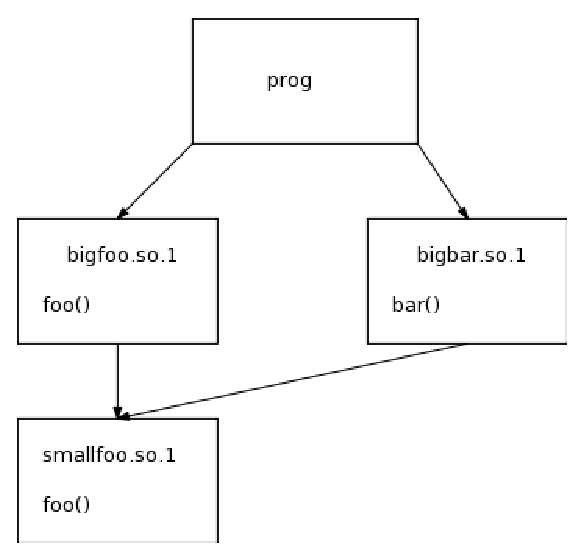
\includegraphics[width=60mm,keepaspectratio]{img/debugging/symbol-search.eps}
%\end{center}

%===============================================================================
\subsection{dtrace}

\begin{itemize}
\item dynamic instrumentation
\item ...
\item Available on: Solaris, FreeBSD, Mac OS X, QNX
\item performance/lock contention debugging
\end{itemize}


\begin{itemize}
\item References:
  \begin{itemize}
  \item dtrace guide
  \item The Solaris Dynamic Tracing (DTrace) Guide:
  \item dtrace(1M) man page
  \end{itemize}
\end{itemize}

\endinput

%===============================================================================
% Terminals.
%===============================================================================

\section{Terminals}

%===============================================================================
\subsection{Terminal I/O Overview}

\begin{itemize}
\item Terminal is an input/output device.
\item You can read from and write to it.
\item Historicaly, it was a hardware device.
\begin{itemize}
	\item Connected to the computer via a serial line.
	\item There was no stderr as we know it now.
	\item A keyboard and a paper roll for displaying text (no video
	displays at the time).
	\item Then, video displays came in (AKA "glass TTYs").
\end{itemize}
\end{itemize}

\begin{itemize}
\item Whatever is displayed on the terminal comes from the terminal driver, ie.
what you type goes right over the serial line to the computer, the input might
be processed in a few different ways, and the output goes back to the terminal
to be displayed -- unless the echo is ``off''. \emsl{The terminal does not
display directly what you type, it always goes through the terminal driver code
running on the computer.}
\item Also note that RS-232, a commonly used standard for serial communication,
is a fully duplex protocol.
\end{itemize}

%===============================================================================
\subsection{Terminal I/O Overview (cont.)}

\begin{itemize}
\item today, a \emph{terminal} usually means a \emph{text terminal}, not a
\emph{physical terminal}
\begin{itemize}
	\item a text terminal usually runs under a graphical environment
\end{itemize}

\item some byte sequences have special meaning
\begin{itemize}
	\item moving the cursor, clearing the screen, etc.
	\item try \texttt{vim >output} and see what is in \texttt{output}
	\begin{itemize}
		\item do not forget to type ``:q'' as well
	\end{itemize}
\end{itemize}

\item different terminals have different capabilities
\begin{itemize}
	\item some cannot clear the screen, for example
	\item types of terminals: ansi, vt100, xterm, ...
\end{itemize}
\end{itemize}

\begin{itemize}
\item You probably know that we can also have virtual terminals on a console.
Most un{}ix-like system support that. Usually you can switch between virtual
terminals by hitting \texttt{Alt + Fx} where \texttt{Fx} is a function key.
	\begin{itemize}
	\item Virtual terminal configuration varies. On BSD systems, you have
	file \texttt{/etc/ttys} to set what virtual (and network) terminals you
	have.
	\end{itemize}
\item UNIX windowing (ie., graphical) environments did not eradicate the
terminal interface since it is very convenient to deal with.
\item Some applications might even refuse to run without a terminal -- screen
oriented editors, for example.
\item When running a terminal in the graphical environment, \texttt{xterm}, for
example, then that is the application that gets the keyboard input. It then
processes the input and sends the filtered data to the shell through a pseudo
terminal. Do not worry about pseudo terminals now, will be explained later.
\item You have to distinguish what is supported by the terminal, the terminal
driver itself, and what is done in the shell. For example, the terminal driver
offers by default \^{}D for ``End-Of-File'', meaning that it will close its
output (usually, shell's input) when \^{}D (binary \texttt{04}) is read
from the terminal, or \^{}S which suspends the output from the driver. However,
\texttt{bash} itself, for example, accepts \^{}L to clear the screen. That means
that \^{}L goes through the terminal and the terminal driver to the shell which
interprets it and sends a ``clear the screen'' sequence back to the terminal, if
the terminal itself supports the feature. \^{}L is not interpreted by the
terminal driver in contrast to \^{}D or \^{}S. More information is on page
\pageref{TERMIOS}.
\item When you hit \^{}C, that character is sent by the terminal application
(eg. \texttt{xterm}) which is interpreted by the terminal driver which generates
the \texttt{SIGINT} signal to the application. That means that neither the
terminal application nor the shell generates that signal. You can verify it like
this -- start \texttt{cat} in your shell. Then, \texttt{truss} your
\texttt{xterm} (not shell! Remember, \texttt{ptree} is great on Solaris for
finding out child-parent relationships. On Linux distros, try ``\texttt{ps
--forest}'') or any other terminal you use. Move your mouse to the terminal
again. You can press \texttt{Ctrl} itself several times to see that there is
some communication between the terminal and X over the X11 socket; use
\texttt{pfiles} to check which file descriptor is the X11 socket. Then, type
\^{}C. You should see something like this:

\begin{verbatim}
write(4, "03", 1)                               = 1
ioctl(3, FIONREAD, 0x08047A50)                  = 0
pollsys(0x080479D0, 2, 0x00000000, 0x00000000)  = 1
read(4, " ^ C", 1024)                           = 2
read(4, 0x08074C4A, 1022)                       Err#11 EAGAIN
\end{verbatim}

The terminal writes \texttt{03} to the terminal because that's what \^{}C is.
\texttt{03} means 1 byte of value 3. Note that \^{}E is \texttt{05} then, \^{}L
is \texttt{12} etc. Be careful that \texttt{truss} shows some characters using
escapes so \^{}J is $\backslash$\texttt{n} (\texttt{0A}, new line), \^{}L is
$\backslash$\texttt{f} (\texttt{0C}, form feed), and \^{}M is
$\backslash$\texttt{r} (\texttt{0D}, carriage return). What you get from the
terminal is literaly ``\^{}C'' in two characters, and that's what you see in
your terminal, literaly. Shell does not send it, that's the (pseudo) terminal
driver. More on this later.
\end{itemize}

%===============================================================================
\subsection{Physical (Hardware) Terminal}

\begin{center}
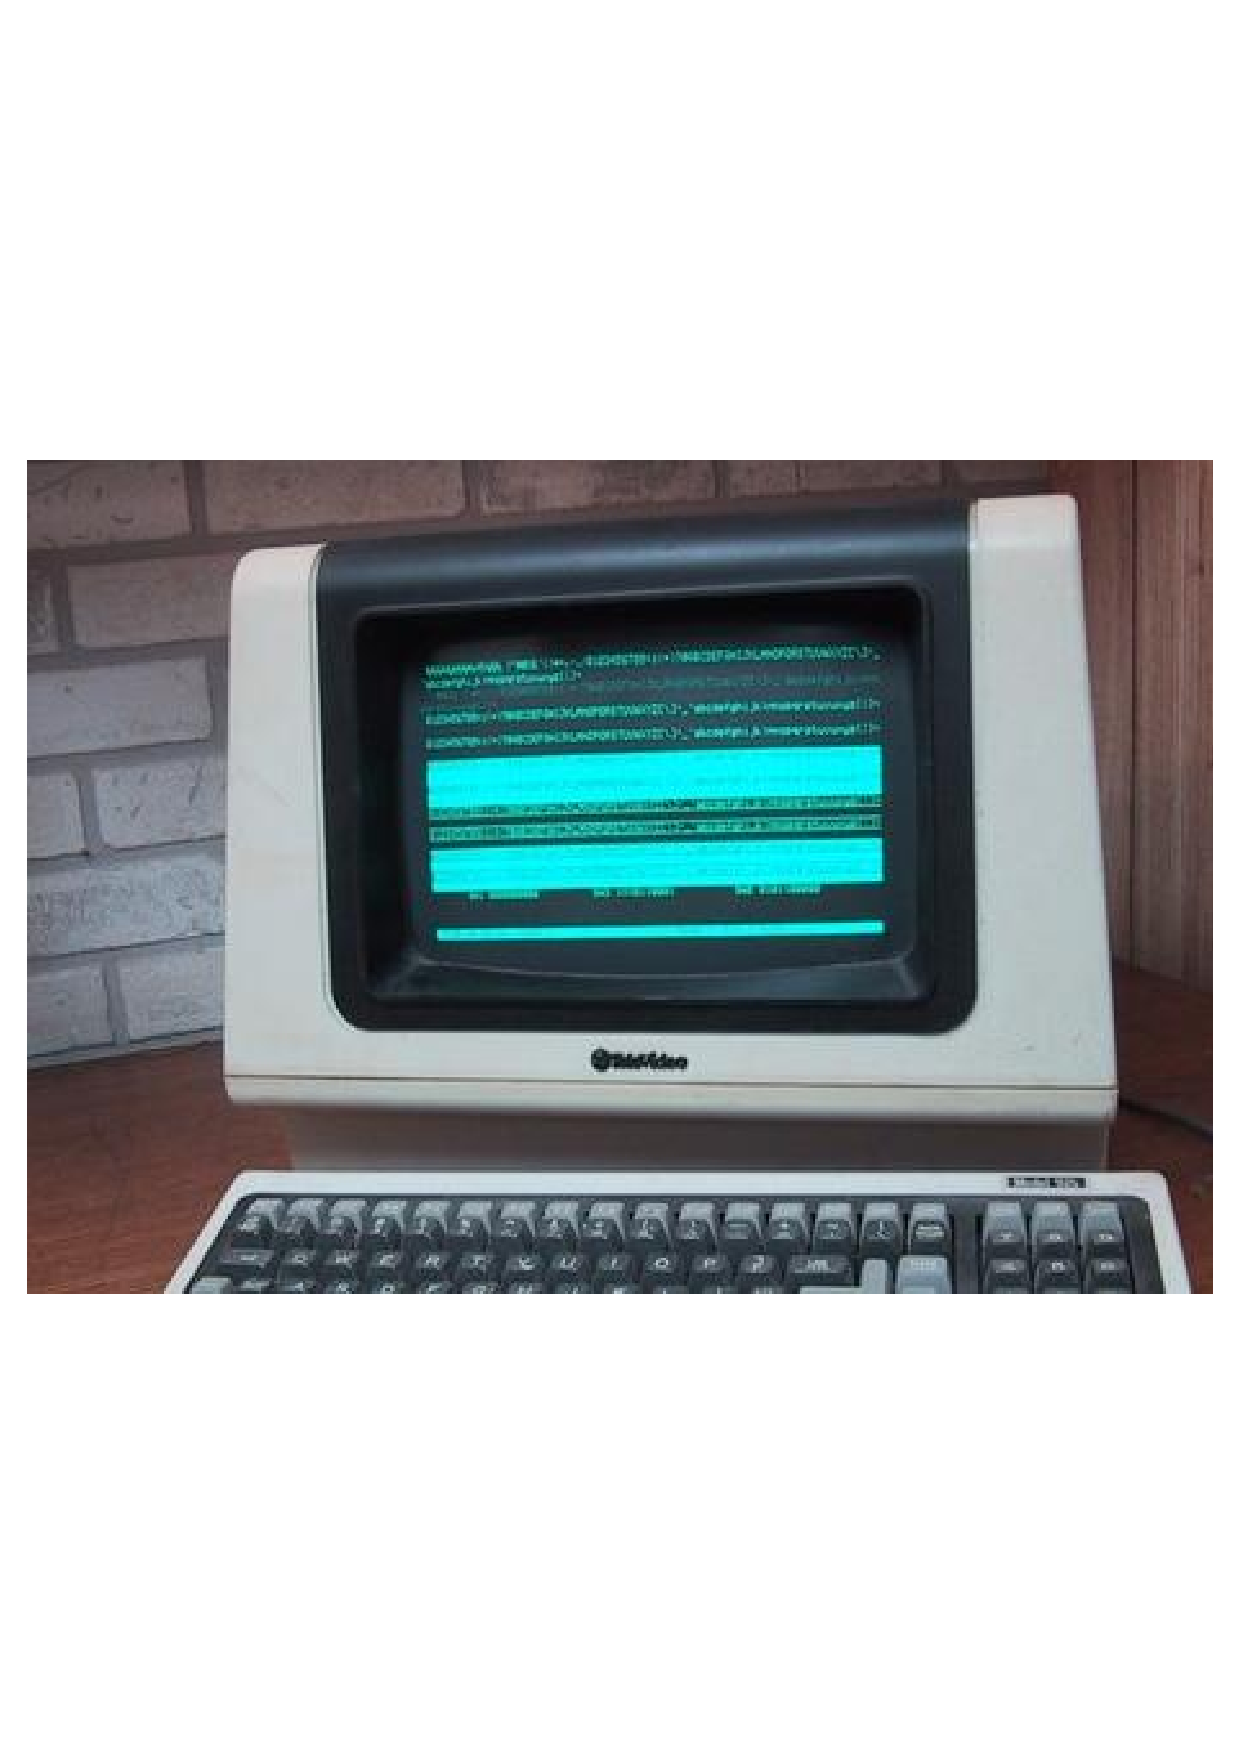
\includegraphics[width=90mm]{img/terminals/Televideo925Terminal.pdf}
\end{center}

\begin{itemize}
\item Picture in public domain downloaded from Wikipedia.
\item Note that while it looks like a ``normal'' computer it is not. It just
communicates with the ``real'' computer over a serial line.
\item As already mention, remember that echo (ie. what you see when you type) on
the terminal display is not done by the terminal itself. The terminal can output
only what it gets from the other side, meaning that the ``remote'' system (= the
terminal driver) itself does that echo for you. This can be switched off via the
\texttt{tcsetattr} function, which will be introduced later. You can use
"\texttt{stty -echo}" from the command line to switch off the echo, and
"\texttt{stty echo}" to switch it on again.
\item Even these days, you might need to use your computer to emulate a physical
terminal. Some devices like Cisco routers and switches might still need to be
configured with the IP address and the gateway using the serial console before
you can log it to it. You can use \texttt{tip(1)} (usually shipped by default
with your UNIX or un{}ix-like system) or myriad of other comms like
\texttt{Minicom} etc.
\end{itemize}

%===============================================================================
\subsection{\texttt{stty}(1) command}

\begin{itemize}
\item changes and prints the terminal line settings
\item \texttt{stty -a}
	\begin{itemize}
	\item lists the settings in a human readable form
	\end{itemize}
\item example
	\begin{itemize}
	\item \texttt{stty -echo} disables echo
	\item \texttt{stty echo} enables echo
	\end{itemize}
\item maybe most useful example of this command
	\begin{itemize}
	\item \texttt{stty sane}
	\item for example, if you paste some rubbish by mistake, and your
	terminal starts acting weird, the \texttt{sane} option often helps.
		\begin{itemize}
	  	\item not every time though
		\end{itemize}
	\end{itemize}
\end{itemize}

\begin{itemize}
\item We will use this command in other examples.
\end{itemize}


%===============================================================================
\subsection{TTY Driver Connected To a Phy Terminal}

\begin{center}
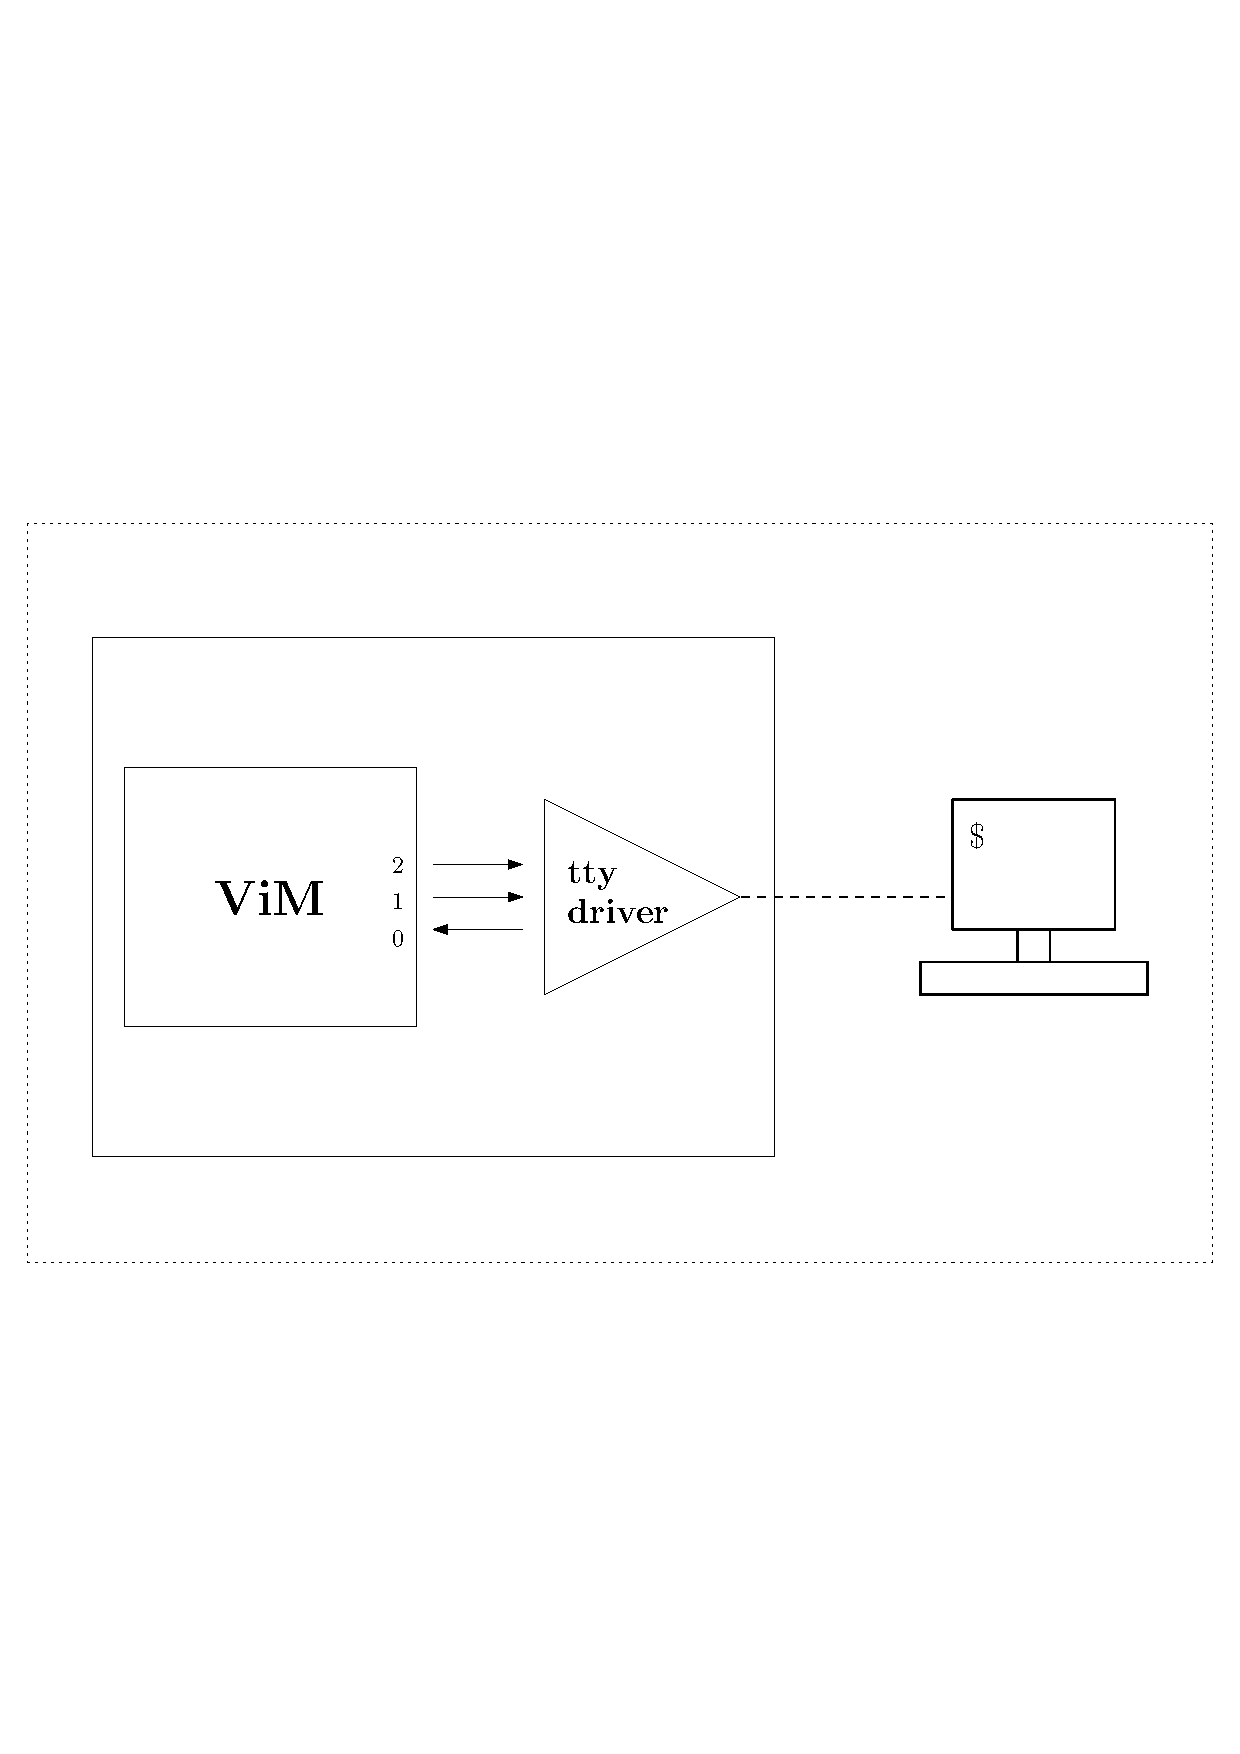
\includegraphics[width=105mm]{img/terminals/working-with-phy-term.pdf}
\end{center}

\begin{itemize}
\item The ViM editor communicates with the terminal driver, the driver takes
care of the communication with the actual physical terminal.
\item This is how it also looks when you run ViM from the virtual console.
\end{itemize}

%===============================================================================
\subsection{Pseudo terminals Overview}

\begin{itemize}
\item pseudo terminal is an emulation of a physical terminal
\item \emsl{allows one process to control another process that is written for a
terminal}
\begin{itemize}
	\item remotely running ViM over an SSH connection, for example
	\item such application (SSH) must support it in order this can work
\end{itemize}
\item you can have multiple (text) terminals on your desktop
\item an application written for a terminal does not care (more or less) whether
it communicates with a physical or a pseudo terminal
\end{itemize}

\begin{itemize}
\item The pseudo terminal device driver acts just like a terminal as far as the
interactive (slave) process is concerned. However, the other end is connected to
a master process, not to the physical device. The master process can read from
the pty master what the application wrote to it, and can write to the pty master
what it wants the application to read from the slave pty.
\item In other words, the master side of the pseudo terminal represents the
physical terminal, the slave part represents the special device end point.
\item The pseudo terminal can not be just one point used by both processes. It
is the same as a (bidirectional) pipe - you need 2 ends so that the processes
can communicate with each other.
\end{itemize}

%===============================================================================
\subsection{PTY Driver Connected To a Process}

\begin{center}
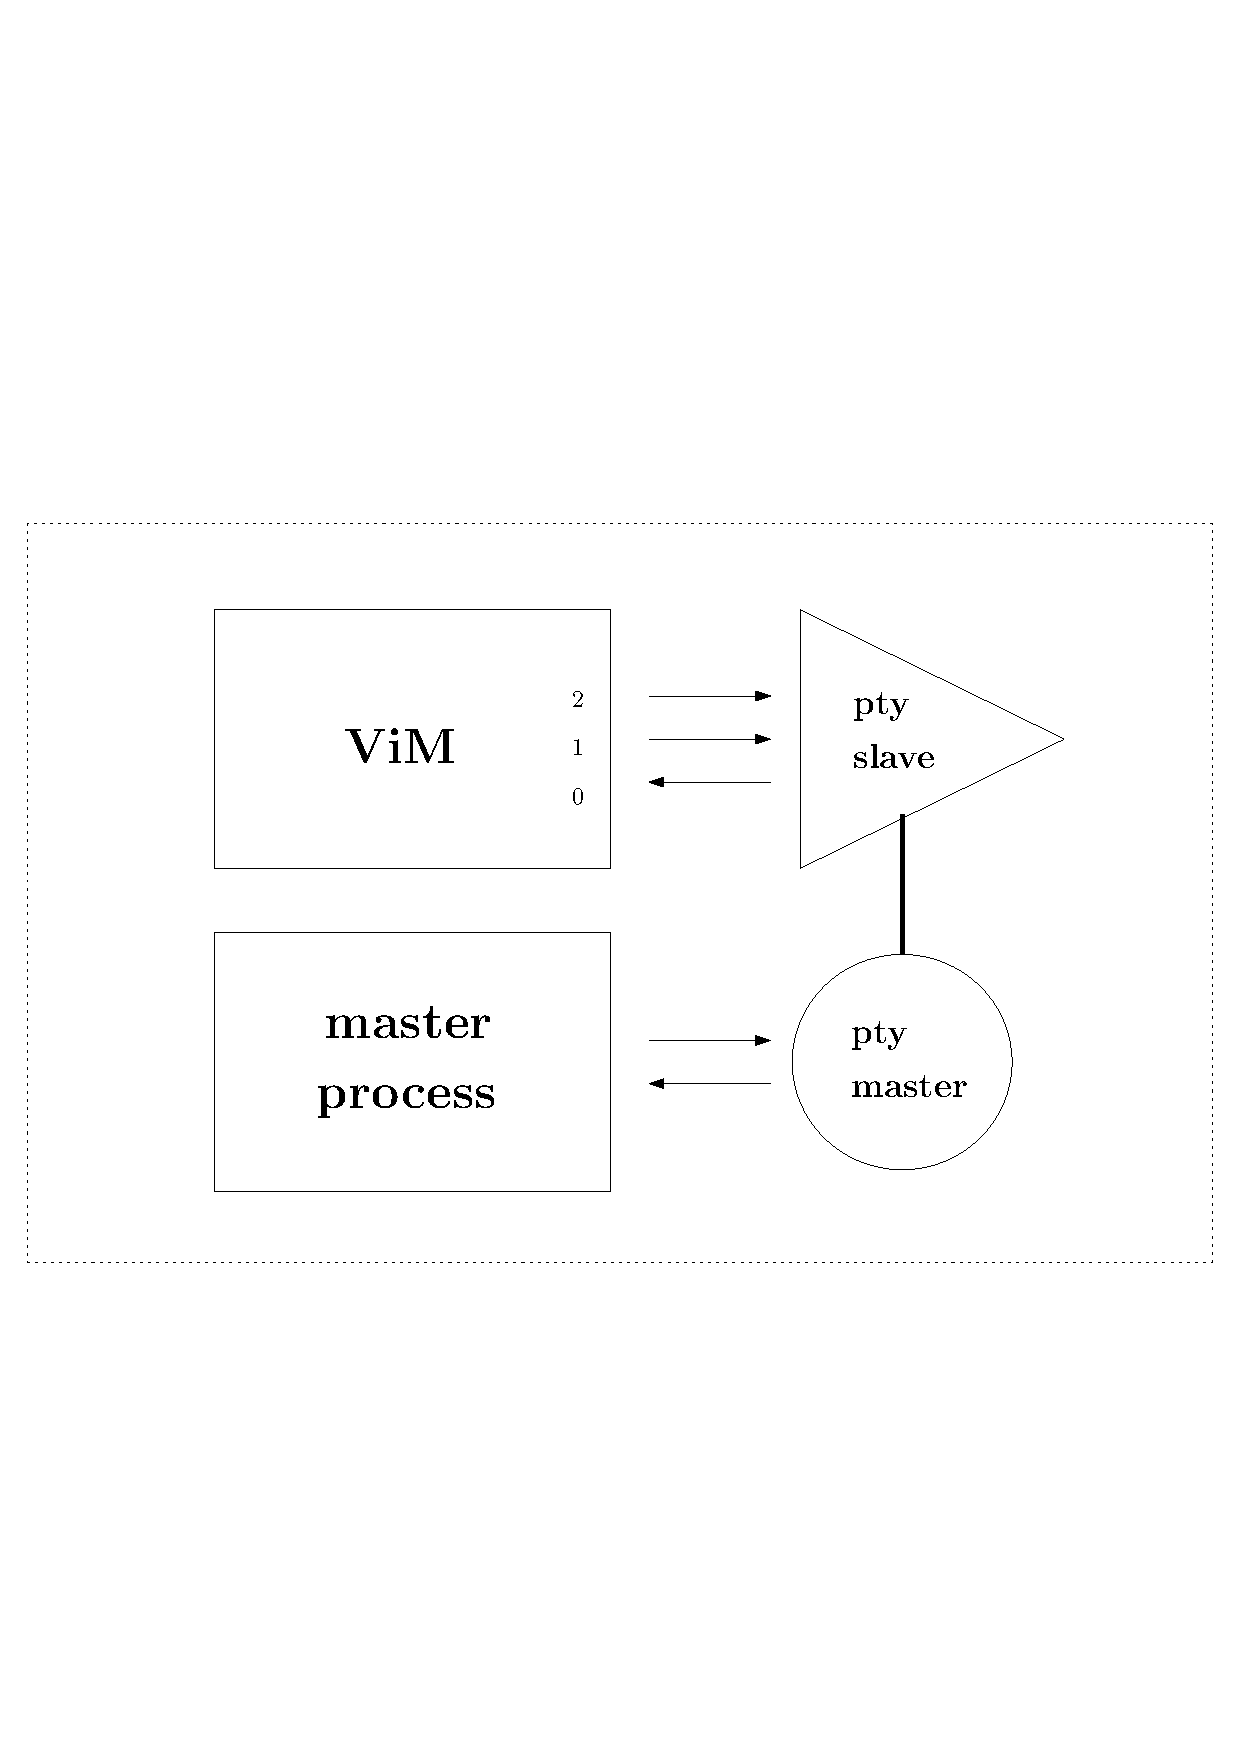
\includegraphics[width=105mm]{img/terminals/working-with-pty.pdf}
\end{center}

\begin{itemize}
\item The master process can be \texttt{xterm}, for example, running a shell
which started the ViM editor. More processes can work with the same terminal, as
we will see later.
\item \emsl{The master process and the master PTY together emulates the physical
terminal.}
\item How to get the pseudo terminal and how to use it in your program will be
explained later in the chapter.
\item How exactly is the slave and the master part ``connected'' together in the
kernel does not have to be of a programmer's concern.
\end{itemize}

%===============================================================================
\subsection{More Complex Example}

\begin{center}
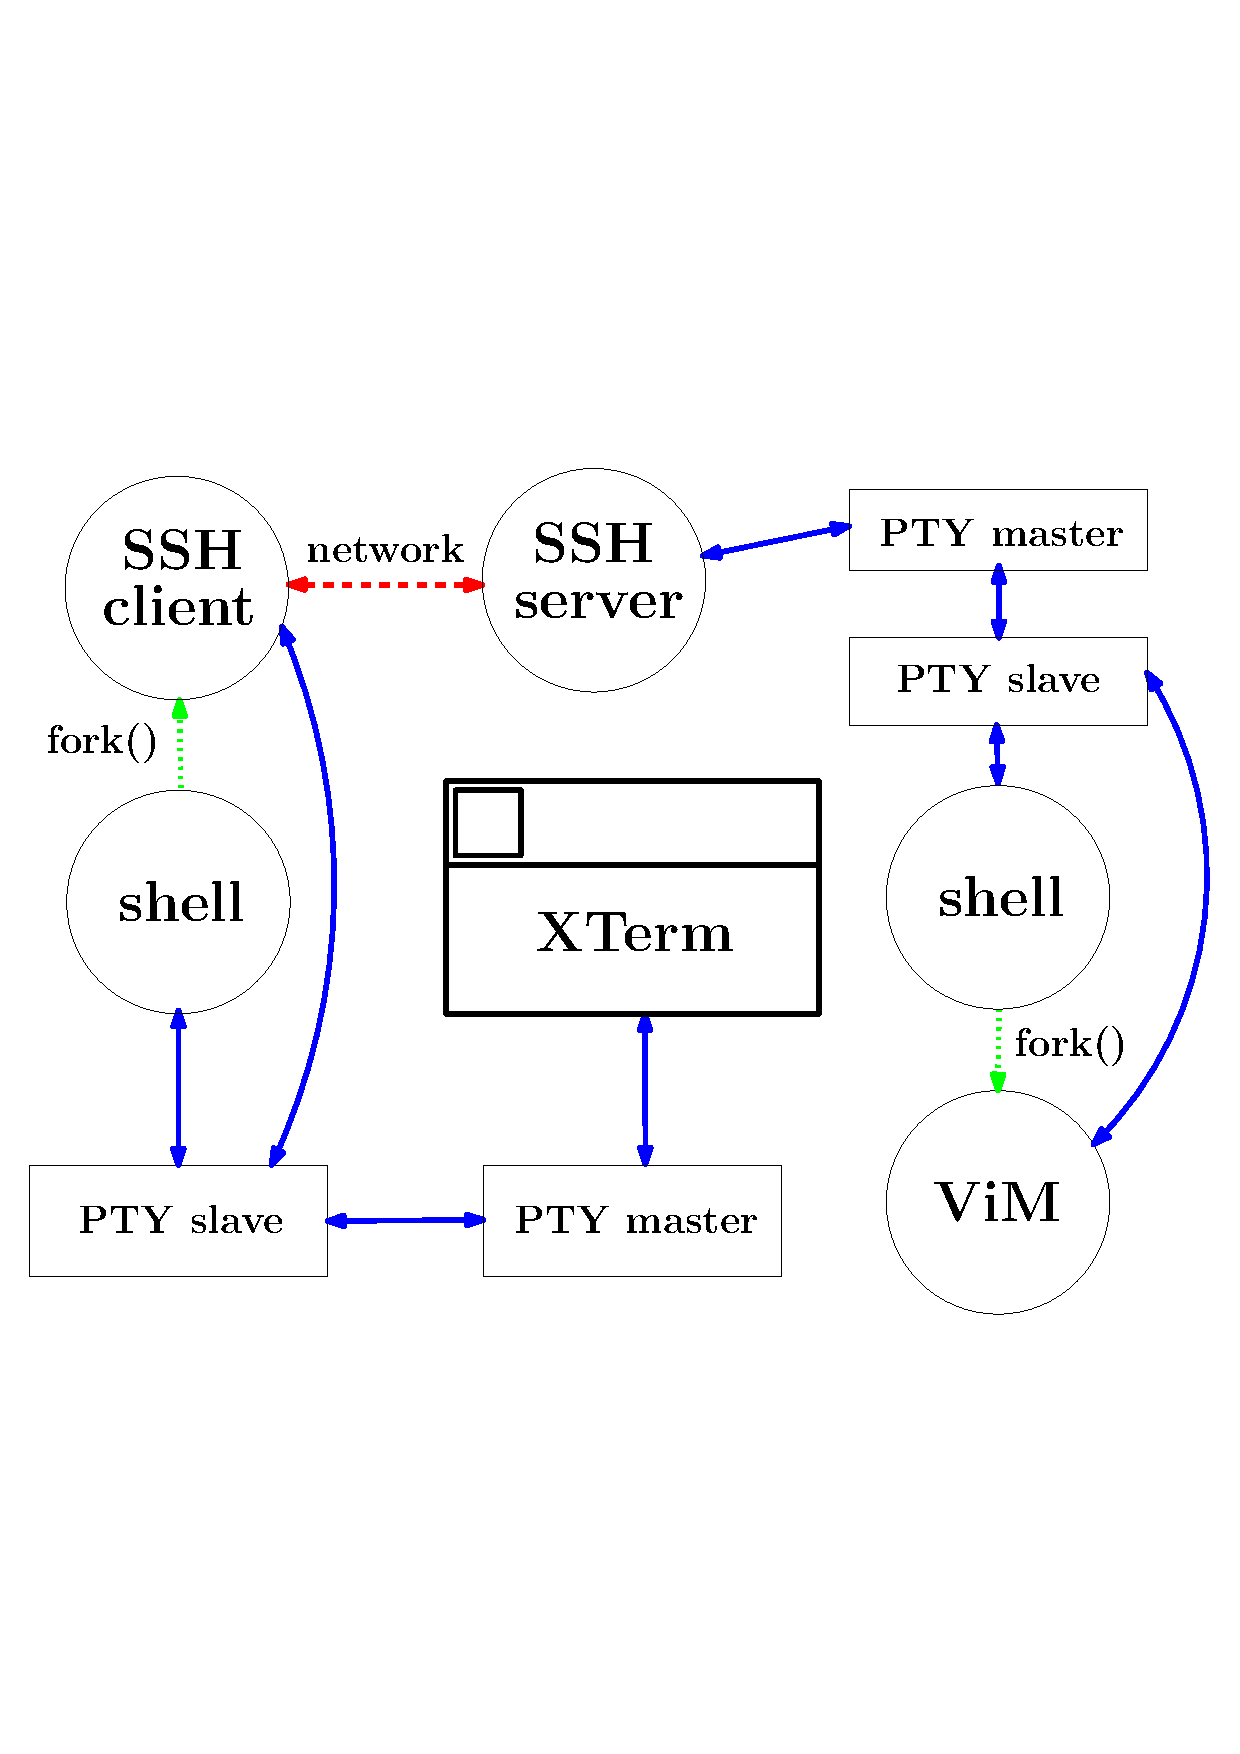
\includegraphics[width=90mm]{img/terminals/remote-vim-with-pty.pdf}
\end{center}


\begin{itemize}
\item The picture shows a situation where an SSH client running from a shell in
a terminal window is connected to the remote side, and running ViM there.
\item Note that ViM is not communicating over the shell. It is reading and
writing to the same terminal as the shell is. It is about process groups and
the controlling terminal as we will see later in the chapter.
\item The communication between the 2 pseudo terminal ends is bidirectional (in
other words, it's full duplex).
\item Question: when user runs ViM over SSH, what is the settings of the slave
pseudo terminal devices on remote and local side?
	\begin{itemize}
	\item Answer: will be the same because SSH transmits all terminal
	settings to the other side, see RFC 4254 above.
	\end{itemize}
\item Example:

\begin{verbatim}
# Get the local pseudo terminal name, remotely log in using
# SSH, get the remote pseudo terminal name there as well,
# and then run ViM.
$ tty
/dev/pts/5
$ ssh localhost
Password: 
$ tty
/dev/pts/8
$ vim 

# And now from another console, check the settings of both
# slave pty's.
$ /usr/gnu/bin/stty --file=/dev/pts/5
speed 38400 baud;
eol2 = M-^?; swtch = <undef>; min = 1; time = 0;
-icrnl
-opost
-isig -icanon -iexten -echo -echoe -echok

$ /usr/gnu/bin/stty --file=/dev/pts/8
speed 38400 baud;
eol2 = M-^?; swtch = <undef>; min = 1; time = 0;
-icrnl ixany
-onlcr tab3
-isig -icanon -iexten -echo -echoe
\end{verbatim}

\end{itemize}

%===============================================================================
\subsection{Reading From a Terminal}

\begin{itemize}
\item normally, the application uses descriptors 0, 1, and 2
\begin{itemize}
	\item those may or may not be connected to a terminal
	\item if not, user probably redirected those, eg.\\
	\texttt{cat /etc/passwd > my\_passwd}
\end{itemize}

\item an application can explicitly open \texttt{/dev/tty}
\begin{itemize}
	\item a synonym for a controlling terminal for the process
	\item the reason to do that might be to read a password and bypassing
	any redirections
\end{itemize}
\item an app can (try to) open actual terminal name (eg., \texttt{/dev/tty02})
\end{itemize}

\begin{itemize}
\item Applications usually do not allow to read a password from a redirected
file for security reasons. However, they might provide a way to do it via a
separate program. For example, look for \texttt{SSH\_ASKPASS} in \texttt{ssh(1)}
manual page.
\item See \priklad{terminals/getpassphrase.c}, read the comment inside. The
program will use the terminal no matter how you redirect the standard input.
And, if you have no terminal at all, it will fail the way as documented in
the manual page for \texttt{getpassphrase(3C)}.
\item Shell command \texttt{tty(1)} prints the controlling terminal:

\begin{verbatim}
$ tty
/dev/pts/15
$ pfiles $$
2256:   bash
  Current rlimit: 256 file descriptors
   0: S_IFCHR mode:0620 dev:342,0 ino:453881557 uid:1629480 gid:7 rdev:24,15
      O_RDWR|O_NOCTTY
      /dev/pts/15
   1: S_IFCHR mode:0620 dev:342,0 ino:453881557 uid:1629480 gid:7 rdev:24,15
      O_RDWR|O_NOCTTY
      /dev/pts/15
   2: S_IFCHR mode:0620 dev:342,0 ino:453881557 uid:1629480 gid:7 rdev:24,15
      O_RDWR|O_NOCTTY
      /dev/pts/15
   3: S_IFDOOR mode:0444 dev:351,0 ino:50 uid:0 gid:0 size:0
      O_RDONLY|O_LARGEFILE FD_CLOEXEC  door to nscd[328]
      /var/run/name_service_door
 255: S_IFCHR mode:0620 dev:342,0 ino:453881557 uid:1629480 gid:7 rdev:24,15
      O_RDWR|O_NOCTTY FD_CLOEXEC
      /dev/pts/15
\end{verbatim}
\end{itemize}

%===============================================================================
\subsection{Reading From a Terminal (cont.)}

\begin{itemize}
\item normally, an application gets input in lines because the terminal driver
does not send the data up until ``Enter'' is hit.
\begin{itemize}
	\item unless the input/output is redirected to/from a non-terminal
\end{itemize}
\item no arrow keys, deletes, backspaces get through to the application. All
that is handled in the driver.
\begin{itemize}
	\item it is said that terminal is in the \emph{canonical mode}
\end{itemize}
\item Ctrl+D at the beginning of the line means ``End of File''. \texttt{read()}
then returns 0 to indicated it.
\end{itemize}

\begin{itemize}
\item For more information on terminal modes, see page \pageref{CANONICAL}.
\item See examples (again, read the comments):
\priklad{terminals/simple-read.c} and
\priklad{terminals/simple-tty-read.c}. The 2nd one does similar thing to what
\texttt{getpassphrase(3C)} does. Try without a terminal to see that.
\item \texttt{O\_NONBLOCK} can be used as usual. Either with \texttt{fcntl()} on
the file descriptor, or directly with \texttt{open()} in which case it also
affects \texttt{read()} as well. See [\myun\myix-prog] for more info.
\item Do not forget that \texttt{select()} and \texttt{poll()} calls are useful
when there is a need to read from more file descriptors without busy waiting.
\end{itemize}

%===============================================================================
\subsection{Sessions and Process Groups (Jobs)}

\begin{itemize}
\item a new \emph{session} is created when the user logs in
\item that new session consists of one \emph{process group}
\item the only process in the process group is the login shell
\begin{itemize}
	\item that is the simple scenario with no windowing environment
\end{itemize}
\item the process is a \emph{process group leader} and a \emph{session leader}
as well
\begin{itemize}
	\item its PID is also a proces group ID and a session ID
\end{itemize}
\item that's how it is today. The history of this was quite colorful and
diverse.
\end{itemize}

\begin{itemize}
\item Some of that was in [\myun\myix-prog].
\item Example to show that my login shell is both the session leader and a
process group leader ("-j" prints session and process group ID as well):

\begin{verbatim}
$ ssh $(hostname)
Password: 

$ ptree $$
503   /usr/lib/ssh/sshd
  4117  /usr/lib/ssh/sshd
    4118  /usr/lib/ssh/sshd
      4124  -bash
        4160  ptree 4124
$ ps -j -p 4124
  PID  PGID   SID TTY         TIME CMD
 4124  4124  4124 pts/10      0:00 bash
\end{verbatim}
\item The pseudo terminal slave, ie. the end used the by the terminal
application (\texttt{bash}), is \texttt{/dev/pts/10}.
\item And, if we use \texttt{pfiles} on the right \texttt{sshd} process, we can
see that the pty master end of the pseudo terminal is also 10 (note
``\texttt{rdev:23,10}'').

\begin{verbatim}
  11: S_IFCHR mode:0000 dev:341,0 ino:56712 uid:0 gid:0 rdev:23,10
      O_RDWR|O_NONBLOCK|O_NOCTTY|O_LARGEFILE
      /devices/pseudo/clone@0:ptm
\end{verbatim}
\item Remember that you can kill a process group with \texttt{kill(2)} by using
a negative number where the number is a process group PID. You can do the same
with \texttt{kill(1)} command: ``\texttt{kill -- -<PGPID>}''. Note that you must
not forget to use ``\texttt{--}'' to stop the command to interpret the process
group PID as an option. Killing the whole process group may come in handy if you
want to kill a big process group like a parallel system build with tens of
processes, etc.
\item \label{BASH_KSH} Try to run ``\texttt{sleep 991 | sleep 992 | sleep 993 |
sleep 994}'' and play with this process group. You can kill it as a group using
the negative number, you can try to kill individual process and see what
happens. Examining the behaviour of \texttt{bash}, for example, it will not
notify you that the job has finished until all processes of the group have
finished. Korn Shell 93 (\texttt{ksh93}), on the other hand, waits on the last
process only. You can also observe that there is a difference in how processes
are created. \texttt{bash} is the father of all processes and starts creating
those from left to right, Korn shell creates the last process in the pipe line
and all other processes in the job are created by it. Given that Korn shell
creates just one process, the group leader, it must create the last one in the
pipe since that assures that shell will wait for the whole pipe to get
completed.
\item \emsl{Exercise:} use Bash and Korn shell with the ``sleep'' job above and
verify the above mentioned information. With the Korn shell, use
\texttt{/bin/sleep} instead of \texttt{sleep} since the latter is a built-in
command in KSH so you would see only \texttt{ksh} in the process listing.
However, you need the seconds to distinguish between individual processes.
\end{itemize}

%===============================================================================
\subsection{Sessions and Process Groups (cont.)}

\begin{itemize}
\item the terminal the user logged in becomes a \emph{controlling terminal} of
the session
\item the session leader is also a \emph{controlling process}
\item if \emph{job control} is enabled, every command or a pipeline forms a new
process group
\begin{itemize}
	\item all such groups have the same controlling terminal, unless the
	application explicitly changes that
\end{itemize}
\end{itemize}

\begin{itemize}
\item See this commented output:
\begin{verbatim}
# Let's see what is in our process tree.
$ ptree $$
503   /usr/lib/ssh/sshd
  4117  /usr/lib/ssh/sshd
    4118  /usr/lib/ssh/sshd
      4124  -bash
        4283  ptree 4124

# Let's run the 1st job, on the background.
$ while true; do sleep 1; echo X; done | wc -l &
[1] 4291

# Let's run the 2nd job, on the background as well.
$ sleep 999 &
[2] 4303

# Let's see what jobs we have.
$ jobs
[1]-  Running   while true; do sleep 1; echo X; done | wc -l &
[2]+  Running   sleep 999 &

# Now, let's see our process tree again.
$ ptree $$
503   /usr/lib/ssh/sshd
  4117  /usr/lib/ssh/sshd
    4118  /usr/lib/ssh/sshd
      4124  -bash
        4290  -bash
          4316  sleep 1
        4291  wc -l
        4303  sleep 999
        4317  ptree 4124

# The following bash process is the process group leader for
# the while loop (note that 'while' is a shell internal
# command so that's why we see 'bash', not 'while' there).
# Also note that all those processes share the same login
# session, with session ID 4124.
$ ps -j -p 4290
  PID  PGID   SID TTY         TIME CMD
 4290  4290  4124 pts/10      0:00 bash

# Note that 'wc' is a member of the above mentioned process
# group as well and it is NOT a process group leader (bash
# with PID 4290 is).
$ ps -j -p 4291
  PID  PGID   SID TTY         TIME CMD
 4291  4290  4124 pts/10      0:00 wc

# However, 'sleep 999' was run as its own job so it formed a
# new process group, with one process in it (sleep) and
# sleep is the process group leader as well. You can also
# see that from the ptree(1) output that we cannot assign
# the commands listed to their respective groups, we must
# use ps(1) to get that additional information.
$ ps -j -p 4303
  PID  PGID   SID TTY         TIME CMD
 4303  4303  4124 pts/10      0:00 sleep
\end{verbatim}
\end{itemize}

%===============================================================================
\subsection{Controlling Terminal}

\begin{itemize}
\item a session can have one controlling terminal. Daemons usually do not have
it.
\item it is the \emsl{first terminal} that a session leader (and a session
leader \emsl{only} can do that) opens after the new session was created
\item the session leader that establishes the connection to the controlling
terminal is called a controlling process
\item terminal input and terminal generated signals go to the foreground group
only
\item if modem (or network) disconnect is detected by the terminal interface,
\texttt{SIGHUP} is sent to the controlling process or group
\end{itemize}

\begin{itemize}
\item A new session is created via calling \texttt{setsid(2)}, see
p\pageref{SETSID}.
\item As to differences between systems and the \texttt{SIGHUP} signal, see
p\pageref{SIGHUP_SIGNAL}.
\item The above says that there are sessions without a controlling terminal,
those sessions usually contain daemons, server processes, etc.
\item The above also says that in order to get rid of a controlling terminal,
you have to create a new session. It is not enough to close the controlling
terminal -- which would usually mean to close stdin, stdout, and stderr. See
\priklad{terminals/close-the-tty.c}. And, if you want to make sure you will
never get a controlling terminal in the session, let the session leader fork and
exit. Since only the session leader can acquire the controlling terminal, and we
have no session leader anymore (just its child), we are safe. Actually, that's
how the \texttt{daemon} call usually works.
\item If the session leader opens a terminal with \texttt{O\_NOCTTY}, such
terminal will not become the controlling terminal.
\item You cannot open \texttt{/dev/tty} to get a controlling terminal,
\texttt{/dev/tty} is a synonym for an already existing controlling terminal.
%\item TODO maybe a similar picture to the one in 9.6 (pic 9.7) of Adv Prog in
%UNIX (Stevens) could be included?
\item How to check that if you Ctrl-C your application the signal will go to the
foreground group and not to the shell? That's easy, get the PID of the shell,
run ``\texttt{sleep 999}'', run ``\texttt{truss -p <PID>}'' on the shell, and
then \^{}C the \texttt{sleep} process. You will see that the shell will get
\texttt{SIGCLD}, not \texttt{SIGINT}.
\item \emsl{Exercise:} write a very simple \texttt{tty} program. Read what
exactly \texttt{tty(1)} does and then use \texttt{truss} to find out what
function to call. It's basically a one-liner. The solution is in
\priklad{terminals/tty.c}.
\end{itemize}

%===============================================================================
\subsection{Job Control}

\begin{itemize}
\item the fact that a process group runs in the background does not mean that it
cannot use the terminal
\begin{itemize}
  	\item however, it can only write to it, cannot read from it
\end{itemize}
\item the "job control" means that certain signals are only sent to the
foreground process group
\begin{itemize}
	\item \texttt{SIGINT} (\texttt{\^{}C}), \texttt{SIGQUIT} (usually
	\texttt{\^}{}$\backslash$, quits and generates a core dump), and
	\texttt{SIGTSTP} (usually \texttt{\^{}Z}, suspends the process)
\end{itemize}
\item the "control" part of job control means that we can move jobs back and
forth between foreground and background, kill them independently of other jobs,
etc.
\item job control as such needs a system support for process groups
\end{itemize}

\begin{itemize}
\item The \emph{foreground process}, or the \emph{foreground group} if there are
more than one process in the group, is defined as process or a group that has an
unlimited access to the controlling terminal.
\item The \emph{controlling group} is a group associated with the terminal. If
job control is enabled, it's the same as the foreground group.
\item Every shell may do that differently but usually internal commands for job
control are "jobs", "fg", and "bg". Also, internal "kill" command can work with
job IDs. See manual page for your shell.
\item See the following bash example on \texttt{kill} shell internal command:
\begin{verbatim}
$ sleep 999 &
[1] 5760
$ jobs
[1]+  Running                 sleep 999 &
# use '%' with the job ID to kill a specific job
$ kill %1
[1]+  Terminated              sleep 999
\end{verbatim}
%\item TODO Put here what the shell does when putting a process to the
%foreground/background.
\end{itemize}

%===============================================================================
\subsection{What Happens If Job Control is Disabled?}

\begin{itemize}
\item in other words, how it was before job control was introduced...
\item you can still run processes in the background
\begin{itemize}
	\item but it means that the shell just does not wait for them
\end{itemize}
\item all processes are part of the same process group as the login shell
\item signals are sent to all processes
\item note that choosing a job control might be a compile time option of your
shell
\begin{itemize}
	\item bash has it like that
\end{itemize}
\end{itemize}

\begin{itemize}
\item Note that when bash is built with "\texttt{configure
--disable-job-control}" (which is not the default setting, obviously), all
commands started in the background will be spawned with \texttt{SIGINT} and
\texttt{SIGQUIT} ignored. That means that \^{}C will not kill them and will kill
only the pipeline in the foreground. That is what a user would most probably
expect. Killing background processes with \^{}C could really suprise the user.
\item \emsl{Exercise:} build Bash w/o the job control and verify the above
stated information. Use \texttt{psig} command on Solaris to see what signal
handlers are installed for commands started in the background.
\end{itemize}

%===============================================================================
\subsection{\texttt{SIGHUP} Signal}

\begin{itemize}
\item if the terminal hangs up or is disconnected, the controlling process
(shell) gets a \texttt{SIGHUP} signal (SVR4)
\begin{itemize}
  	\item or, the whole controlling group gets the signal (BSD)
\end{itemize}
\item usually, \texttt{SIGHUP} terminates the shell
\begin{itemize}
	\item in SVR4 though, the shell itself is expected to send
	\texttt{SIGHUP} to to \emsl{foreground group} before it exits
\end{itemize}
\item the shell \emsl{may} send \texttt{SIGHUP} to all processes in the session then
\begin{itemize}
	\item that's why you might need to start remote jobs with "\texttt{nohup
	<job>}" if you want them to survive the logout
	\item \texttt{ksh} and \texttt{bash} do that, not sure about other
	shells
\end{itemize}
\end{itemize}

\label{SIGHUP_SIGNAL}

\begin{itemize}
\item On Solaris, try the following. Start two \texttt{sleep} processes, one in
the foreground, one in the background:

\begin{verbatim}
$ echo $$
4104
$ sleep 888 &
[1] 4150
$ sleep 999
\end{verbatim}

and see how the process tree looks like from another terminal:

\begin{verbatim}
$ ptree 4104
...
...
  2659  /usr/local/bin/rxvt -fn fixed
      4104  bash
        4150  sleep 888
        4154  sleep 999
\end{verbatim}

Now, truss both \texttt{sleep} processes and the shell as well. When you kill
the terminal window which simulates the terminal disconnect, you will see that
the foreground \texttt{sleep} processes got \texttt{SIGHUP}s from the shell:

\begin{verbatim}
$ truss -p 4154
pause()                         (sleeping...)
    Stopped by signal #24, SIGTSTP, in pause()
    Received signal #15, SIGTERM, in pause() [default]
      siginfo: SIGTERM pid=4104 uid=1629480
pause()                                         Err#4 EINTR
\end{verbatim}

The \texttt{sleep} process in the background continues to run.
However, the shell gets the signal from the kernel (the terminal driver) since
there is no PID, and then it sent the signals to all existing process groups:

\begin{verbatim}
$ truss -p 2881
waitid(P_ALL, 0, 0x08047AA0, WEXITED|WTRAPPED|WSTOPPED|WCONTINUED) (sleeping...)
    Received signal #1, SIGHUP, in waitid() [caught]
...
...
kill(-2716, SIGHUP)                             = 0
kill(-2735, SIGHUP)                             = 0
\end{verbatim}

\item Note that there is a difference between a shell getting a \texttt{SIGHUP}
or a shell exiting. For example, if \texttt{bash} exits, it sends a
\texttt{SIGHUP} to the controlling group only (if you type \texttt{exit}, the
controlling group would be empty since no foreground process is running).
However, if you set the \texttt{huponexit} option; it sends \texttt{SIGHUP} to
all processes. You can verify it easily -- start \texttt{sleep 888} in the
background, truss it from another terminal, and exit the shell. The terminal
window disappears but the \texttt{sleep} process continues to run without
getting any signal.

\item There are significant differences between systems, expecially between
older systems, about how they deal with terminals, process groups, and such.
\item SVR3 (1986)
\begin{itemize}
	\item the session usually consisted of 1 process group, and terminal
	could be associated with only one group. Thus, if a new group was
	created, the (new) process leader was disconnected from the controlling
	terminal and had to open another one.
	\item however, it could still use it through already open file
	descriptors, no \texttt{SIGHUP} would be sent on death of the leader
	though (see below).
	\item also, process group could not close the controlling terminal and
	later allocate another one (screen(1) would not work there)
	\item on death of the group leader the kernel sends \texttt{SIGHUP} to
	all processes in the group, those processes lose the terminal and also
	the group ceases to exist (group ID of the processes is zeroed out)
	\item when the terminal is disconnected the driver sends \texttt{SIGHUP}
	to all processes in the session
	\item no job control possible		  	
	\item many other differencies from what we are used to today
\end{itemize}

\item 4.3BSD (1986)
\begin{itemize}
	\item a process can change its group ID
\begin{itemize}
		\item thus we can have process groups without a leader
\end{itemize}
	\item more groups can share the same controlling terminal
\begin{itemize}
		\item but the terminal can control just one group
\end{itemize}
	\item background process gets \texttt{SIGTTIN} on read (will suspend it
	by default)
	\item background process can write to a terminal (or get
	\texttt{SIGTTOUT} if the terminal is configured that way)
	\item when the terminal is disconnected the driver sends \texttt{SIGHUP}
	to the controlling group (only)
	\item on session end, \texttt{vhangup()} is used on the controlling
	terminal to traverse the process table, all the terminal entries are
	made unusable, then it \texttt{close()} the terminal, and
	\texttt{SIGHUP} is sent to the controlling group.
\begin{itemize}
		\item that's why on, for example, FreeBSD all background
		processes survives the logout.
\end{itemize}
	\item however, there is no notion of a controlling process as it was in
	SVR3.
\end{itemize}

\item SVR4 (1990)
\begin{itemize}
	\item have sessions and process groups
	\item controlling terminal is associated with a session and a foreground
	process group
	\item only session leader may allocate and deallocate a controlling
	terminal
\end{itemize}
\end{itemize}

%===============================================================================
\subsection{So called hang-on-exit problem}

\texttt{\$ ssh bash\_user@hostname "sleep 10 \&"}

\begin{itemize}
\item the above hangs for 10 seconds on Solaris and Linux
\item however, it does not on FreeBSD, OpenBSD, and NetBSD
\begin{itemize}
	\item in both cases though, the shell itself exits immediatelly
	\item so, why the hang?
\end{itemize}

\item SSH sleeps in \texttt{select()}, waiting on an event on the terminal
\begin{itemize}
	\item and on Solaris and Linux, it does not get the end-of-file when the
	shell exits. See notes for more info.
\end{itemize}

\item bash's \texttt{huponexit} prevents the hang on Solaris and Linux but for
the price of \texttt{SIGHUP} killing the process
\end{itemize}

\begin{itemize}
\item On BSD, \texttt{revoke()} is used to revoke all descriptors using the
terminal, and SSH daemon thus gets 0 (end-of-file) on \texttt{read()}. And,
\texttt{sleep(1)} still runs after the connection closes.
\item On Solaris and Linux, that does not happen since there is no
\texttt{revoke()}, so the \texttt{sleep(1)} command keeps the terminal open
which is why the SSH daemon does not get end-of-file till \texttt{sleep(1)}
exits.
\item You should definitely try it yourself on those systems.
\item See a discussion on OpenSSH mailing list. Look for
"so-called-hang-on-exit" and especially for the subject "The complete answer
(was Re: so-called-hang-on-exit)" by Nico Williams; it has a lengthy
explanation of the problem:\\
\url{http://marc.info/?l=openssh-\myun\myix-dev&m=102878253003241&w=2}
\item On Solaris:
\begin{verbatim}
$ ssh localhost
$ sleep 99 &
[1] 4552
$ logout
<HANGS HERE UNTIL THE SLEEP CMD EXITS>
\end{verbatim}

However, if you use the \texttt{huponexit} option in \texttt{bash}:

\begin{verbatim}
$ ssh localhost
$ shopt -s huponexit
$ sleep 99 &
[1] 4552
$ logout
Connection to localhost closed.
\end{verbatim}
\end{itemize}

%===============================================================================
\subsection{Function calls for sessions and process groups}

\texttt{int \funnm{setsid}(void);}
\begin{itemize}
\item creates a new session, with the current process as a session leader
\end{itemize}
\texttt{int \funnm{setpgid}(pid\_t \emph{pid}, pid\_t \emph{pgid});}
\begin{itemize}
\item sets the process group ID \texttt{pgid} for process \texttt{pid}
\end{itemize}
\texttt{int \funnm{getsid}(pid\_t \emph{pid});}\\
\texttt{int \funnm{getpgid}(pid\_t \emph{pid});}
\begin{itemize}
\item get the session or process group ID of process with PID \texttt{pid}
\end{itemize}

\begin{itemize}
\item \label{SETSID} The process calling \texttt{setsid} must not be a process
group leader. \texttt{EPERM} is returned otherwise.
\item New session has no controlling terminal. That's perfect for daemons since
they do not need any.
\item Normally, you can use \texttt{daemon()} call to daemonize your app which
does the right thing. It might not be available on your system so the way how to
do it is this:
	\begin{itemize}
	\item fork()
	\item the parent exits
	\item the child calls setsid()
	\item and redirects 0/1/2 file descriptors from/to \texttt{/dev/null}
	(ie., it opens \texttt{/dev/null}, \texttt{dup2()} it to 0/1/2, and
	closes it again).
	\end{itemize}
\item Source code example: \priklad{terminals/daemonize.c}.
\end{itemize}

%===============================================================================
\subsection{Opening a Terminal}

\begin{itemize}
\item On a classic terminal login each configured terminal is managed by
\texttt{init}, followed by \texttt{getty} and \texttt{login}.
	\begin{itemize}
	\item And \texttt{getty} is run with the terminal name as a parameter so
	it knows which terminal to open. It initializes the line, reads the user
	name and \texttt{exec()}s \texttt{login} with the username as a
	parameter.
	\end{itemize}

\item On networks logins and on terminals that are run through your windowing
environment, pseudoterminals are used.
	\begin{itemize}
	\item You ask for a new pseudoterminal then. More on that soon.
	\end{itemize}

\end{itemize}

\begin{itemize}
\item By classic terminal login we mean sitting in front of a black screen with
"Login:" only.
\item By configured terminals we mean even virtual terminals used usually via
Alt-Fxx keys from the text console.
\end{itemize}

%===============================================================================
\subsection{Working with Pseudoterminals}

\begin{itemize}
\item different on different systems
\item however, POSIX defines functions that should be used
	\begin{itemize}
	\item systems map their native calls to POSIX calls:
	\end{itemize}
\end{itemize}

\begin{verbatim}
posix_openpt() - open a master pseudo terminal device
grantpt()      - changes the ownership of the corresponding
                 slave device to the calling UID
unlockpt()     - unlock the corresponding slave device so
                 that it can be read/written from/to
ptsname()      - gets the name of the corresponding slave
                 device
\end{verbatim}


\begin{itemize}
\item \texttt{xterm} uses \texttt{posix\_openpt()}, \texttt{grantpt()}, and
\texttt{unlockpt()}.
\item \texttt{xterm} forks, calls \texttt{pstname()} to get the slave device,
and redirects 0/1/2 to the slave for the child.
\item xterm's child \texttt{exec()}s the shell.

\item For example, Linux gets the master pseudo terminal by calling
\texttt{getpt(3)}, Solaris by opening \texttt{/dev/ptmx} etc.
\texttt{posix\_openpt()} is then implemented by those native function calls.

\item On Solaris, the app needs to push \texttt{ptem} and \texttt{ldterm}
modules onto the slave side to get terminal semantics.
	\begin{itemize}
	\item pty's are implemented using STREAMS on Solaris
	\item see the example code
	\end{itemize}
\item Source code example on how one process can communicate with another
process over a newly allocated pseudo terminal: \priklad{terminals/pty.c}.
\end{itemize}

%===============================================================================
\subsection{Setting Terminal Attributes}

\begin{itemize}
\item various terminal attributes can be set
	\begin{itemize}
	\item terminal speed, uppercase to lowercase conversion, remapping
	various control characters, echo switch off/on, etc.
	\end{itemize}
\item \funnm{tcgetattr}(), \funnm{tcsetattr}()
\item canonical versus punctual mode
	\begin{itemize}
	\item normally, input characters are queued until a line is complete, as
	indicated by pressing an Enter
	\item in the punctual mode, there is no line queing.
	\end{itemize}
\item raw mode is punctual with many other attributes switched off, including
ECHO
	\begin{itemize}
  	\item editors usually operate in raw mode
	\end{itemize}
\end{itemize}

\label{CANONICAL}
\label{TERMIOS}

\begin{itemize}
\item The terminal attributes are set using the \texttt{termios} structure that
is used as a parameter of a subsequent \texttt{tcsetattr()} call. The structure has
input (eg. enable start/stop input control), output (eg. map CR to NL on
output), control, and local modes (eg. enable echo on/off). Then it has an array
of control characters (EOF, INTR, START, STOP, SUSPEND, ...) mapped to
characters  -- usually \^{}D, \^{}C, \^{}Q, \^{}S, \^{}Z, respectively.
\item So, if you want to be able to generate EOF with \^{}X instead of \^{}D,
you would use ``\texttt{stty eof \^{}X}''. \texttt{stty(1)} would change
\texttt{termios.c\_cc[VEOF]} to \texttt{24} and then set the new structure via
\texttt{tcsetattr()} with command \texttt{TCSANOW} (Change Attributes Now), for
example. See \texttt{termios.h} in the UNIX spec for more information on all
required terminal control characters.
\item Raw mode with no ECHO is used when you type a password, for example,
and want to print * for every character typed. You could not do that in the
canonical mode. See the \texttt{ICANON} flag in \texttt{c\_lflag} of the
\texttt{termios} structure. Also, see \texttt{MIN} and \texttt{TIME} params. For
more information, consult manual page for \texttt{termio(7I)}.
\item There is no single attribute to set for the raw mode. See \texttt{-raw}
option in \texttt{stty(1)} man page for the list of attributes switched off/on
for that mode.
\item Some old terminals could print only uppercase. To input/output an
uppercase then, the letter is preceded by a backslash.
\item Example on how to switch the echo off: \priklad{terminals/no-echo.c}.
Note that it is independent on whether we use a physical terminal or a pseudo
terminal. That means that we work with the terminal driver which is the slave
part in case of pseudo terminals. That is the part that echos the characters
read from the terminal.
\item \emsl{Exercise:} you can modify the \texttt{no-echo.c} code so that you
can read the password and print * for each character typed. It's fine to ignore
all special characters like backspace, arrows, etc. You will have to switch off
the canonical mode and use \texttt{c\_cc} field of the \texttt{termio} structure
to set those \texttt{MIN} and \texttt{TIME} parameters. Hint -- when used as
indexes, you prepend \texttt{V} to them. Solution:
\priklad{terminals/type-password.c}. Read \texttt{termio} manual page for
more information.
\end{itemize}

%===============================================================================
\subsection{Terminfo database}

\begin{itemize}
\item a database describing the capabilities of devices such as terminals and
printers
\item devices are described by specifying a set of capabilities and character
sequences that trigger them
\item screen oriented apps (eg., \texttt{vim}) and other commands (eg.,
\texttt{ls}) use \emsl{generic} capabilities without a need to know the exact
terminal used
\item terminfo source files are converted into a database by the \texttt{tic}(1)
command
\item terminfo source files are usually in \texttt{/usr/share/lib/terminfo}
\end{itemize}

\begin{itemize}
\item Terminfo capabilities:
	\begin{itemize}
	\item Boolean capabilities
		\begin{itemize}
		\item Whether the terminal has the feature or not.
		\item Eg., can clear the screen.
		\end{itemize}
	\item Numeric capabilities:
		\begin{itemize}
		\item Quantifying a particular feature of a device.
		\item Eg., number of columns in a line
		\end{itemize}
	\item String capabilities:
		\begin{itemize}
		\item Providing sequences used to perform particular operations
		on devices.
		\end{itemize}
	\end{itemize}
\item terminfo is an System V equivalent of the original \emph{termcap} system
born in the BSD world. The termcap was invented by Bill Joy after he wrote the
first version of the \texttt{vi} editor. After the ininitial version of the
editor was written for a specific terminal, users started to want ports of the
editor for different terminals. Instead of bending the editor for each
available terminal, Bill Joy rewrote the editor with generic commands to
manipulate the terminal, and introduced a \emph{termcap} database containing
capabilities of various terminals, and a library to query the database.
\item termcap is a text based database, usually in \texttt{/etc/termcap}, see
FreeBSD, for example. It is just one file. Terminfo is a compiled database,
built from a separate files, one for each terminal. It might not come with the
source files used to build the database. On Solaris, it is in
\texttt{/usr/share/lib/terminfo}. It contains subdirectories named after letters
to accomodate hundreds of terminals in an easy way.
\item you can use \texttt{infocmp} to display the contents of the terminfo
entry:

\begin{verbatim}
$ infocmp vt100
#       Reconstructed via infocmp from file:
#       /usr/share/lib/terminfo/v/vt100
vt100|vt100-am|dec vt100 (w/advanced video),
    am, mir, msgr, xenl, xon,
    cols#80, it#8, lines#24, vt#3,
    acsc=``aaffggjjkkllmmnnooppqqrrssttuuvvwwxxyyzz{{||}}~~,
    bel=^G, blink=\E[5m$<2>, bold=\E[1m$<2>,
...
...
\end{verbatim}

\item For example, \texttt{am} means ``automargin'', ie. when a line reaches the
right edge of the screen, the terminal automatically continues on the next line.
\texttt{cols\#80} says that the terminal has 80 columns.
\item Example: move the cursor to the specified position when the terminal is
\texttt{xterm}. Solution is in \priklad{terminals/move-cursor-on-xterm.c}.
You can set \texttt{PS1} to an empty string to see that the cursor will get to
the absolute position then.
\item \emsl{Exercise:} clear the screen and then move the cursor to the
specified position on any supported terminal. Use low level terminfo routines to
do that. Those routines are beyond the scope of this lecture, read apropriate
documentation if you are interested. However, it is recommended to use
\emph{curses} which is a higher level interface. Anyway, the solution to
experiment with is here: \priklad{terminals/move-cursor-with-terminfo.c}.
\end{itemize}

\endinput

%===============================================================================
% Advanced Network Programming.
%===============================================================================

\section{Advanced Network programming}

beyond the "listen on a socket and accept requests"

%===============================================================================

\subsection{Accessing low level structures}

\begin{itemize}
  \item get a list of interfaces on the system (ala ifconfig(1M)) (1)
  \begin{itemize}
    \item OpenBSD: getifaddrs(3) - get list of IPs on the system
    \item Solaris: ioctl() interface and \texttt{SIOCGLIFNUM},
      \texttt{SIOCGLIFCONF} (2)
  \end{itemize}
\end{itemize}


\begin{itemize}
  \item[(1)] e.g. to listen on each individual address in the system
  \begin{itemize}
    \item handy when the reply has to have the right source address
      (e.g. NTP protocol)
    \item need to track down the changes while running (see the
      \texttt{PF\_ROUTE} socket slide)
  \end{itemize}
  \item[(2)] Generic approach of copying out sequence of structures from
    the kernel to userland:
\begin{enumerate}
  \item open \texttt{AF\_INET}/\texttt{SOCK\_DGRAM} socket
  \item fill the lifnum structure
  \item issue the \texttt{SIOCGLIFNUM} ioctl to get number of interfaces
  \item allocate buffer for number of entries acquired in previous step
  \item fill the lifconf structure
  \item issue the \texttt{SIOCGLIFCONF} ioctl to get interface structures
  \item traverse the list of lifreq structures
\end{enumerate}
  \item \texttt{lifreq} is defined in \texttt{usr/src/uts/common/net/if.h}
and contains various interface specific data:
\begin{itemize}
  \item name
  \item physical info
  \item address info
  \item MTU
\end{itemize}
  \item {\bf Example}: \priklad{adv-net-prog/ifclist/}
\begin{enumerate}
	\item compile
\begin{verbatim}
	   make clean && make
\end{verbatim}
	\item run for both address families
\begin{verbatim}
	   ./getlist 4
	   ./getlist 6
\end{verbatim}
	\item compare the output from the list of interfaces
\begin{verbatim}
	   ifconfig -a
\end{verbatim}
\end{enumerate}
{\bf Task}: adjust \texttt{ifclist} to print out IPv4/IPv6 addresses
  on the interfaces
\end{itemize}


%===============================================================================

\subsection{More setsockopt() options}

\begin{itemize}
  \item \texttt{SO\_SNDBUF}/\texttt{SO\_RCVBUF} - performance tuning (1)
  \item \texttt{SO\_EXCLBIND} - exclusive binding (2)
  \item \texttt{SO\_KEEPALIVE} (3)
  \item \texttt{SO\_DONTROUTE} - append ifc name and send to the wire (4)
  \item \texttt{IPPROTO\_IPV6} + \texttt{IPV6\_V6ONLY}
  \item \texttt{IPPROTO\_TCP} + \texttt{TCP\_NODELAY}
  \item \texttt{IP\_SEC\_OPT} - use IPsec per-socket (per-port) policy,
    including policy bypass (5)
\end{itemize}


%	- (janp) zajimavy priklad by byl ukazat na dummy-like netu, ze high
%	  latency, high bandwidth link benefituje hodne ze zvetseni TCP window
%	  atd.

\begin{itemize}
  \item some of the socket options are OS specific
  \item[(1)] we can set {snd,rcv}buf not only for TCP/UDP sockets but also
	  for ICMP (raw ICMP socket)
  \item[(2)] related to security (XXX find the SSH security bug with
    AF\_INET6/AF\_INET fallback)
  \item[(3)] mention OpenSSH and the distinction of Keepalive messages
	on application layer
%	XXX zminit, ze TCP keepalive je hlavne pro detekci crashu celych stroju.
  \item[(4)] gets full control over sending together with RAW sockets
	  - see ping(1M) and -r option
  \item[(5)]
  \begin{itemize}
    \item {\bf Example}: \priklad{adv-net-prog/setsockopt/policy-bypass.c}
\begin{enumerate}
		 \item compile
		 \item run the program w/out bypass
\begin{verbatim}
	    ./bypass 0 20.0.0.1 80
\end{verbatim}
		 \item set policy
\begin{verbatim}
	    echo "{ raddr 20.0.0.1 rport 80 } ipsec
	      { encr_auth_alg sha1 encr_alg aes }" > /tmp/mypolicy.conf
	    chmod 644 /tmp/mypolicy.conf
	    ipsecconf -f -a /tmp/mypolicy.conf
\end{verbatim}
	         \item run the program w/out bypass again
\begin{verbatim}
	    ./bypass 0 20.0.0.1 80
\end{verbatim}
		 \item run the program with bypass
\begin{verbatim}
	    ./bypass 1 20.0.0.1 80
\end{verbatim}
\end{enumerate}
  \item {\bf Example}: \priklad{adv-net-prog/setsockopt/auth.c}
		   \begin{itemize}
		   \item similar to policy-bypass.c but provides traffic 
                   authentication
		   \end{itemize}
		 \begin{enumerate}
		 \item setup IKE
		    XXX
                 \item initiate traffic
		 \end{enumerate}
  \item References:
    \url{http://blogs.oracle.com/danmcd/entry/put\_ipsec\_to\_work\_in}
  \end{itemize}  
\end{itemize}  
%XXX
%	- byl bych opravdu velmi opatrny s IPsecem, vetsina lidi nebude o tom
%	  skoro nic vedet. Napriklad ja o tom skoro nic nevim krome opravdu
%	  zakladnich veci.


%===============================================================================

\subsection{Raw sockets}

\begin{itemize}
  \item bypass packet encapsulation, i.e. push our own headers on the wire
    \begin{itemize}
      \item this is for layer-3/network control
      \item for layer-2/link access PF\_PACKET interface is needed (1)
    \end{itemize}
  \item \texttt{SOCK\_RAW} is a type of socket (see socket(3socket))
    \begin{itemize}
      \item can be used in various domains (will focus on PF\_INET)
    \end{itemize}
  \item need to know packet header format and protocol specifics (2)
\end{itemize}


%	XXX
%		- hmm, neni tomu moc rozumnet. Pouzivani "need to know" se mi
%		  zda trochu nejasny. Melo by tam spis byt "you must know..."
%		  nebo "programmer must know" nebo tak. "need to know" se plete
%		  s klasifikaci utajeni dokumentu.

\begin{itemize}
  \item[(1)] works on Linux, Solaris
  \item[(2)] complete+correct IP header will be needed for most of the cases
    \begin{itemize}
    \item this means we have to compute the checksum
    \item we're pushing stuff to the wire, hence correct byte ordering is
        necessary (\texttt{htons()} etc, see byteorder(3socket))
    \end{itemize}
  \item[(3)] if we need application layer protocols we can let the stack to
    build IP header for us
    \begin{itemize}
    \item ICMP
\begin{verbatim}
    socket(PF_INET, SOCK_RAW, IPPROTO_ICMP)
\end{verbatim}
    \item TCP
\begin{verbatim}
    socket(PF_INET, SOCK_RAW, IPPROTO_TCP)
\end{verbatim}
    \item UDP
\begin{verbatim}
    socket(PF_INET, SOCK_RAW, IPPROTO_UDP)
\end{verbatim}
    \end{itemize}
\end{itemize}

{\bf Example}: construct ICMP packet header with arbitrary type and code
	 \texttt{adv-net-prog/raw-socket}
\begin{enumerate}
	 \item compile
\begin{verbatim}
    make clean && make
\end{verbatim}
	 \item construct ICMP echo request
\begin{verbatim}
    ./icmpraw 20.20.10.10 8 0
\end{verbatim}
\end{enumerate}

%- OS specifics 
%  - endianess in header fields
%  - boundaries of what is allowed to push

\begin{itemize}
\item libnet is a good C wrapper for raw socket manipulation
  \begin{itemize}
    \item \url{http://sourceforge.net/projects/libnet-dev/}
    \item \url{http://www.securityfocus.com/infocus/1386}
  \end{itemize}
\end{itemize}

%XXX
%	- chybi tu par odkazu na na RFC pro IP apod.


%===============================================================================

\subsection{Layer-2 (link) access}

\begin{itemize}
  \item possible choices for link layer access:
    \begin{itemize}
      \item Datalink Provider Interface (DLPI) - Solaris
      \item \texttt{SOCK\_PACKET} - Linux
      \item Berkeley Packet Filter (BPF) - almost everywhere
    \end{itemize}
  \item libpcap
    \begin{itemize}
      \item high-level interface to packet capture
        \item wrapper for all the 3 choices above - OS independent interface
      \item pcap(3)
    \end{itemize}
\end{itemize}


%	XXX
%		- chybi mi tu kratka motivace. Napr. ze chci cist, co na siti
%		  bezi na port 80 atd., at si pod tim muzou neco predstavit.
%		- myslim ze by se hodil i obrazek, jak to obecne cely funguje.

\begin{itemize}
  \item Sequence of steps:
  \begin{enumerate}
    \item find capturing device: pcap\_lookupdev() (optional)
    \item get packet capture descriptor and open the device for capture:
      pcap\_open\_live()
      - alternatively open a file with stored traffic: pcap\_open\_offline()
    \item get network address and mask for the interface: pcap\_lookupnet()
      - will be needed for compiling the filter
    \item compile the filter: pcap\_compile()
    \item put the filter into effect: pcap\_setfilter()
    \item read the data: pcap\_loop()/pcap\_next()
  \end{enumerate}
  \item {\bf Example}: how to integrate pcap into an application
	 \priklad{adv-net-prog/packet-capture}
	 Capture and interpret TCP segements:
  \begin{enumerate}
	 \item compile
\begin{verbatim}
	    make clean && make
\end{verbatim}
	 \item run
\begin{verbatim}
	    ./tcptraffic host www.ms.mff.cuni.cz and port 80
\end{verbatim}
	 \item initiate some traffic
\begin{verbatim}
	    echo "GET /" | nc -w 10 www.ms.mff.cuni.cz 80
\end{verbatim}
	 \item see the output
  \end{enumerate}
  \item Resources:
    \begin{itemize}
      \item UNIX network programming, volume 1 (Richard W. Stevens),
         29 Data link access
    \end{itemize}
\end{itemize}



%===============================================================================

\subsection{Porting applications to IPv6}

\begin{itemize}
  \item or alternatively - writing portable applications
  \item or better - address family agnostic applications
  \item AF-specific data structures (avoid if possible (1)):
    \begin{itemize}
      \item \texttt{AF\_INET} (IPv4): \texttt{sockaddr\_in},
         \texttt{in\_addr\_t}
      \item \texttt{AF\_INET6} (IPv6): \texttt{sockaddr\_in6},
         \texttt{in6\_addr\_t}
    \end{itemize}
  \item AF-agnostic data structures:
    \begin{itemize}
      \item \texttt{sockaddr}, \texttt{sockaddr\_storage} (2)
    \end{itemize}
  \item AF-specific functions (avoid):
    \begin{itemize}
      \item \texttt{gethostbyname()}, \texttt{gethostbyaddr()}
    \end{itemize}
  \item AF-agnostic functions:
    \begin{itemize}
      \item \texttt{getaddrinfo()}, \texttt{getnameinfo()}
    \end{itemize}
\end{itemize}


% XXX obrazek datovych struktur s pretypovanim

% idea: kdyz zacinam psat novy sitovy program, tak co je potreba mit na
%       pameti a udelat, aby aplikace byla rovnou funkcni i pro IPv6.

\begin{itemize}
  \item[(1)] Sometimes it is not possible to avoid AF-specifics
  \item[(2)] de{}fine in \texttt{/usr/include/sys/socket\_impl.h} (will be
  included with \texttt{<sys/socket.h>})
\end{itemize}

{\bf Example}: Watch out when listening on \texttt{AF\_UNSPEC} sockets:
\begin{itemize}
  \item CVE-2008-1483 in SunSSH (CR 6684003)
  \item \url{http://src.opensolaris.org/source/history/onnv/onnv-gate/usr/src/cmd/ssh/libssh/common/channels.c}
  \item \texttt{x11\_create\_display\_inet()} does the setup for X11 forwarding
    over SSH channel
  \item it works like this: \priklad{adv-net-prog/ipv6-port-bind/cycles.c}
\begin{lstlisting}
    for port in (low, high); do
        list = resolve(port for all address faimilies)
        for family in list; do
            create socket for family
            bind the socket to the port and family
            if the bind fails
                if the list is non-empry
                    continue
                      (try the same port number with different address family)
                else
                    try next port number
                fi
            else
                record the port number
            fi
        done
    done
\end{lstlisting}
  \item resolving will produce list with IPv6 family entry first and IPv4
    entry second
  \item if someone binds the port to IPv6 \emph{only} then \texttt{bind()}
    for IPv4 will succeed
    \begin{itemize}
    \item the forwarder thinks everything is okay and passes the port number
    \end{itemize}
  \item the app will try to connect to that port
    \begin{itemize}
    \item some will try IPv6 first but that is hijacked by the attacker
      (who key steal keystrokes in case of X11 connection etc.)
    \end{itemize}
\end{itemize}

%   XXX add attacker app (use nc ?)


%===============================================================================

\subsection{PF\_ROUTE socket}

\begin{itemize}
\item exists on BSD, Linux, Solaris
  \begin{itemize}
    \item PF\_ROUTE exists since 4.3BSD-Reno
  \end{itemize}
  \item usage: routing daemons, network server programs which need to observe
        changes in local addresses and logical interfaces (adding/removing
        server instances)
\end{itemize}


\begin{itemize}
  \item Solaris man pages:
  \begin{itemize}
    \item routing(7P)
    \item route(7P) - describes \texttt{PF\_ROUTE} interface
  \end{itemize}
  \item working with the socket (passive mode):
\begin{enumerate}
  \item open new socket
\begin{verbatim}
     socket(PF_ROUTE, SOCK_RAW, 0);
\end{verbatim}
  \item enter event loop watching for new messages: select/poll + read
  \item processing messages
\end{enumerate}
\end{itemize}

{\bf Example}: write something like 'route monitor' (see route(1M)) but only
    for watching interface additions/removals
     - useful for managing per-address server instances (e.g. UDP servers)
%	 XXX - server instances? To nejak nechapu.
         \priklad{adv-net-prog/routing-socket/}
\begin{enumerate}
  \item compile
\begin{verbatim}
      make clean && make
\end{verbatim}
  \item run
\begin{verbatim}
      ./rtwatch
\end{verbatim}
  \item create new interface (has to plumb IPv6 interface first, then add logical)
\begin{verbatim}
      ifconfig iprb0 inet6 plumb up
      ifconfig iprb0 inet6 addif 2001:0db8:3c4d:55:a00:20ff:fe8e:f3ad/64 up
\end{verbatim}
  \item observe the messages emitted by rtwatch
\end{enumerate}


%===============================================================================

\subsection{PF\_KEY socket}

\begin{itemize}
  \item analogous to the PF\_ROUTE socket
  \item available in Solaris, BSD
    \begin{itemize}
      \item man page: pf\_key(7P)
    \end{itemize}
  \item manipulates IPsec Security Associations (SAs) (1) from userland
  \item app says ADD/DELETE/UPDATE SAs to the kernel
  \item \texttt{PF\_KEY} interface described in RFC 2367
  \item there is also \texttt{PF\_POLICY} socket on Solaris which manipulates
    security policy kernel entries
    \begin{itemize}
      \item which decide whether packet will be allowed, denied or changed (2)
    \end{itemize}
\end{itemize}


\begin{itemize}
  \item[(1)] SAs src/dst description, contain key material, timing information
    etc.
    \begin{itemize}
      \item SA is unidirectional
      \item they are used for computing authentication data and/or encrypt
        packets on the wire
    \end{itemize}
  \item[(2)] simple per-port (per-application) firewall
\end{itemize}

{\bf Example}: flush IPsec AH SAs
	 \priklad{adv-net-prog/key-socket/}
\begin{enumerate}
	 \item compile the program
\begin{verbatim}
	    make clean && make
\end{verbatim}
  	 \item Use Example \priklad{adv-net-prog/setsockopt/auth.c} to set IPsec SAs
         \item observe SAs in the system and start watching
\begin{verbatim}
	    ipseckey dump
	    ipseckey monitor
\end{verbatim}
	 \item flush the AH SAs using our program
\begin{verbatim}
	    ./ahflush
\end{verbatim}
         \item check
\begin{verbatim}
	    ipseckey dump
\end{verbatim}
\end{enumerate}

\begin{itemize}
  \item References:
    \url{http://blogs.oracle.com/danmcd/entry/pf\_key\_in\_solaris\_or}
\end{itemize}


\endinput

%===============================================================================
% Advanced Thread Programming.
%===============================================================================

\section{Advanced Thread Programming}

\begin{itemize}
\item Quick Recapitulation of Threads
\item Other Existing Implementations of Threads
\item \texttt{fork()} and Threads
\item More on Thread Cancellation
\item MT-Level Attributes
\item Solaris Threads API
\item Threads and Performance
\end{itemize}

%\begin{itemize}
%\item ~
%\end{itemize}

%===============================================================================

\subsection{Very Quick Recap of Threads}


\begin{quote}
Multithreading is a programming and execution model that allows multiple threads
to co-exist within the context of a single process. All threads share the
process' resources but are able to execute independently. Threads provide
developers with a useful abstraction of concurrent execution.

% empty para
~

However, perhaps the most interesting application of the technology is when it
is applied to a single process to enable parallel execution of threads on a
multiprocessor system.
\end{quote}


\begin{itemize}
\item Great introduction to threads including some of the history around
this technology can be found in document ''Multithreading in the Solaris
Operating Environment''.
\end{itemize}

%===============================================================================

\subsection{Very Quick Recap of Threads (cont.)}

\begin{itemize}
\item main differences between a thread and a process
\item per thread attributes -- instruction counter, stack, thread ID, ...
\item when to use processes and when to use threads
\item type of implementations of threads
	\begin{itemize}
	\item user-level library (through \texttt{setjump}/\texttt{longjump}
	calls), inherently M:1
	\item kernel (1:1)
	\item hybrid (M:N)
	\end{itemize}
\end{itemize}

\begin{itemize}
\item M:1 means that multiple threads are mapped to one process only. Thus, the
kernel does not know about those threads at all, and in fact does not need to
support any kernel threads. If one thread blocks, the whole process would block
so a thread user-level library must replace blocking function calls with
non-blocking ones.
\item Hybrid M:N approach could be quite difficult to implement, you may be
mapping, say, 23 threads used by your application to 5 kernel threads. The idea
was to use as many threads as needed while not doing so many kernel switches
between those. However, you need two schedulers, for example -- one that
schedules the kernel threads, and one that schedules the user threads. Solaris
abandoned this approach, and NGPT (see page \pageref{NGPT}) was not chosen as
the replacement LinuxThreads library, see below. It seems that much simpler 1:1
approach is generaly the winning one.
\item The assumption that a kernel context switch must be inherently more
expensive than a thread context switch in user level might be tricky. You must
do a lot of things the same whether it is a switch in the kernel or in user
space, and the user space switch typically involves several system calls anyway
- you need to poll to see if the upcoming potentially blocking call is going to
block or not, and if it is then you need to save the current state and use a
long jump to switch to another thread. And there is more to it, see the
reference below.
\item Since FreeBSD 7, an alternative threading library there is
\texttt{libkse(3)} which is M:N. The default threading library is still 1:1
\texttt{libthr(3)} though.
\item References:
	\begin{itemize}
	\item See [\myun\myix-prog] for more information on thread basics.
	\item Very good discussion on M:N versus 1:1 mapping:
	\url{http://xiao-feng.blogspot.com/2008/08/thread-mapping-11-vs-mn.html}
	\end{itemize}
\end{itemize}

%===============================================================================

\subsection{What we know (from POSIX API)}


\begin{itemize}
\item actions we already know how to perform
	\begin{itemize}
	\item creating, destroying, joining, and terminating threads, and
	setting thread attributes when creating a thread
	\end{itemize}
\item synchronization primitives we know
	\begin{itemize}
	\item mutexes, conditional variables, read-write locks
	\item POSIX semaphores were not in [\myun\myix-prog] but it is just an
	analogy to SysV semaphores
	\item barriers
	\end{itemize}
\item what else then do we need to know?
\end{itemize}

\begin{itemize}
\item {}[\myun\myix-prog] went through almost everything from [posix-threads].
\item \label{THREAD_RECAP} \emsl{Exercise:} to get your hands dirty with
threads again, without use of any existing source code files write a simple
program that creates two threads. Each thread writes a ``Hello world''-like
message on stdout to prove that the thread was really created, and then returns.
The main thread waits on both threads to complete before it returns. Writing
that should take 2 minutes and 20 lines of code :-).
\end{itemize}

%===============================================================================

\subsection{Other Implementations}

\begin{itemize}
\item Solaris Threads
\item protothreads
	\begin{itemize}
	\item low-overhead approach, non-preemptable threads with no stack
	\item context is hold in global variables
	%\item provide sequential flow of control
	\end{itemize}
\item POSIX user-space library implementation in FreeBSD 3.0
\item GNU Portable Threads (pth API)
	\begin{itemize}
	\item highly portable user-space threading library (M:1) implementation
	\item can emulate POSIX Thread API as well
	\end{itemize}
\item C Threads API (Mach OS)
\item and many, many more...
\end{itemize}

\begin{itemize}
\item ``Non-preemtable'' in protothreads means that a context switch can take
place on blocking operations only (\texttt{read()}, for example). No stack means
no local variables. Protothreads are targeted at severely memory constrained
systems, such as small embedded systems or wireless sensor network nodes but its
use it not limited to just that.
\item LinuxThreads was a partial implementation of POSIX Threads that has since
been superseded by the Native POSIX Thread Library (NPTL). LinuxThreads had many
problems owed directly to its implementation; each thread had its own PID, for
example, which is a violation of the POSIX standard. NPTL is fully incorporated
in the GNU C library now.
\item Linux version 2.4 had no real kernel thread support.
\item \label{NGPT} GNU Pth and NPTL are two distinct implementations. NPTL makes
use of the Linux kernel threads. There was also NGPT M:N aproach intended to
replace LinuxThreads but eventually NPTL was chosen (BTW, it is 1:1). Read more
on history of Linux threads on the Onlamp link below.
\item User-space implementation of threads, or ``user threads'', not relying on
the system thread support and able to run on systems without such a support at
all, is sometimes called ``green threads''. This seems to have come from the
Java world:

\begin{quote}
\emph{When Java 1.0 first came out on Solaris, it did not use the native Solaris
library libthread.so to support threads. Instead it used runtime thread support
that had been written in Java for an earlier project code-named ``Green.'' That
threading library came to be known as ``green threads.''}
\end{quote}
\item References:
	\begin{itemize}
	\item \url{http://en.wikipedia.org/wiki/Thread\_(computer\_science)}
	\item \url{http://en.wikipedia.org/wiki/LinuxThreads}
	\item \url{http://en.wikipedia.org/wiki/Native\_POSIX\_Thread\_Library}
	\item \url{http://onlamp.com/onlamp/2002/11/07/linux\_threads.html}
	\item protothread implementation: \url{http://www.sics.se/~adam/pt}
	\end{itemize}
\end{itemize}

%===============================================================================

\subsection{Fork and Threads in POSIX}

\begin{itemize}
\item discussed to some extent already in [\myun\myix-prog]
\item \texttt{fork} duplicates only the calling thread in the child
	\begin{itemize}
	\item was not true on Solaris 9 or earlier with Solaris Threads
	\item it used the ``fork all'' semantics (\texttt{forkall(2)}), as
	opposed to the ``fork one''
	\end{itemize}
\item fork-one safety issues
	\begin{itemize}
	\item when \texttt{fork} is used, threads must be well behaved
	\item imagine a thread that does not call \texttt{fork} but holds a
	mutex
		\begin{itemize}
		\item the thread will not be duplicated, leaving the mutex
		locked for ever
		\item the child will probably dead-lock sooner or later
		\end{itemize}
	\end{itemize}
\end{itemize}

\begin{itemize}
\item Remember that a locked mutex may be unlocked only by the thread that
locked it before. That's the difference between a mutex and a binary
se\-ma\-pho\-re.
\item The class of problems that can happen on fork are in general called ``fork
safety issues''.
\end{itemize}

%===============================================================================

\subsection{Memory Leaks on \texttt{fork(2)}}

\begin{center}
% XXX convert to PDF
% 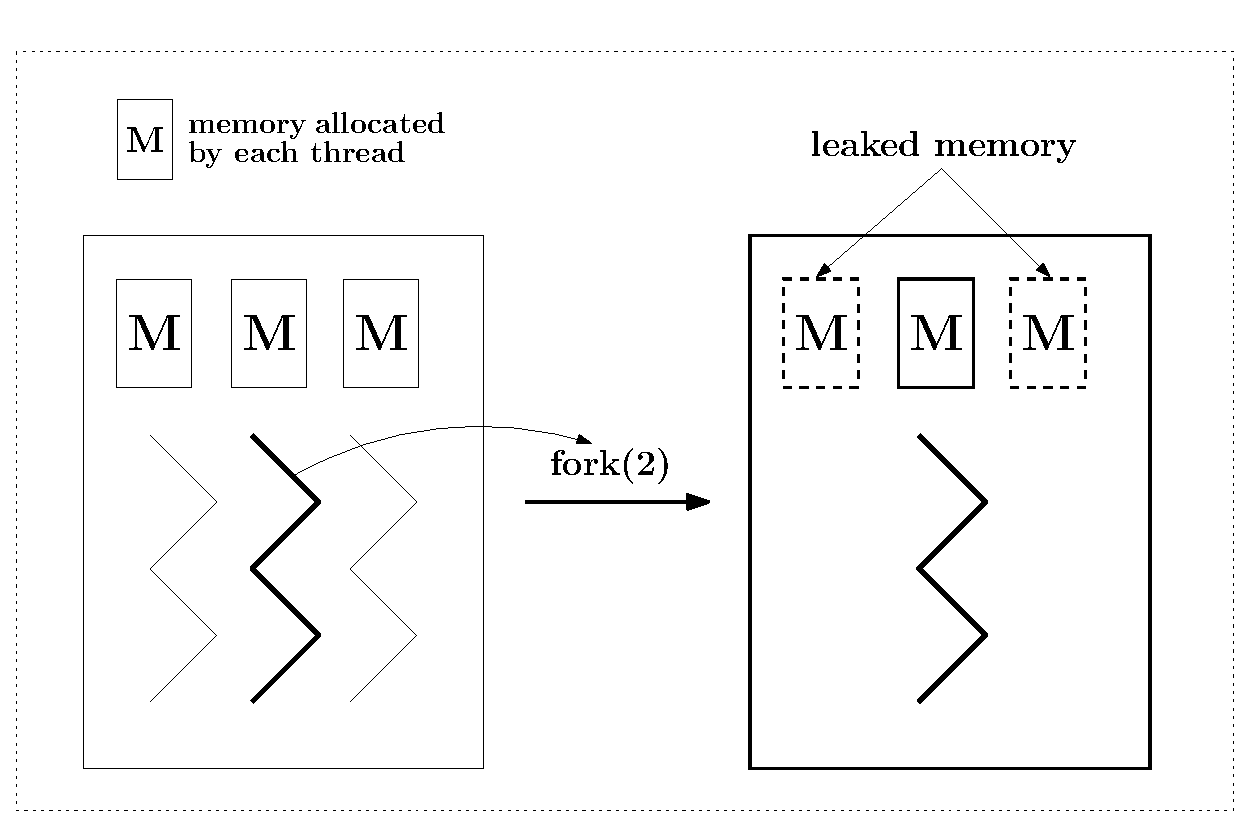
\includegraphics[width=100mm]{img/adv-thread-prog/mem-leaks-with-fork.eps}
\end{center}

\begin{itemize}
\item If a pointer to some memory dynamically allocated in each thread is on the
thread's stack only, such memory will be leaked if the thread is not the one
calling \texttt{fork(2)}. It happens in such a way because the thread, including
its stack, is not duplicated in the new process.
\end{itemize}

%===============================================================================

\subsection{Fork handlers - solution to fork-one safety issues}

\begin{verbatim}
int pthread_atfork(void (*prepare)(void),
                   void (*parent)(void),
                   void (*child)(void));
\end{verbatim}

\begin{itemize}
\item \texttt{prepare} is called before \texttt{fork} is started
\item \texttt{parent}/\texttt{child} are called in parent/child after
\texttt{fork}
\item \texttt{prepare} acquires all mutexes making sure no thread can hold any
lock
\item \texttt{parent}/\texttt{child} functions will release all locks after the
\texttt{fork} then
\end{itemize}

\begin{itemize}
\item Source: \texttt{adv-thread-prog/fork-one-issue.c} shows memory leaks in
the child, \texttt{adv-thread-prog/at\-fork.c} shows how to use the handlers in
general.
\item You may use fork handlers with a process with the \texttt{main()} thread
only, of course, which make them quite a general tool to use.
\item It is not just about mutexes and memory leaks. Imagine a library that has
some kernel state (ie. a handler to some kernel table slot):
	\begin{itemize}
	\item A \texttt{fork} will duplicate the user-level data.
	\item Kernel state will stay the same but now we have 2 processes with a
	handler to the same slot in a kernel table (which holds a reference
	counter equal to 1, not 2).
	\item When one process releases the handler the other thread one can no
	longer work with it since the reference counter dropped to 0, leading to
	the slot deallocation.
	\item For example, PKCS\#11 fork safety issues stem from the fact that
	according to the spec, the child should never use crypto sessions
	initialized in the parent.
		\begin{itemize}
		\item At-fork handlers can help here as well. The sessions are
		closed and initialized again (= the child will get its own
		kernel state structures) in the atfork functions.
		\end{itemize}
	\end{itemize}
\item \texttt{pthread\_atfork()} is not a necessary solution for
\texttt{fork-one-issue.c}. Given you cannot give any parameters to those
functions, global memory would have to be used to store all the pointers anyway
so that we could free those in the child. That means that (a) mdb would show no
memory leaks and (b) we could free all the pointers in the child after the fork.
However, we would have to do that manually which might not be possible -- we
could fork in a library function without knowing about it, for example.
\item In a threaded application, you usually need to fork only to run an
external command, either explicitly or implicitly through a library call. If you
need to do something else you create a new thread, not a new process, so those
problems with mutexes might seem quite unreal -- the external command can not
use those mutexes at all. However, the example above, about PKCS\#11, shows a
real example of a library that uses PKCS\#11 API, and an application that knows
nothing about it while forking a child. That's how SunSSH uses the OpenSSL
PKCS\#11 engine to offload crypto operations to the hardware accelerator. You
must be careful not to create a dead-lock in the library then.
\item Source: another example showing what happens if we hold a mutex in a
thread that has not called \texttt{fork},
\texttt{adv-thread-prog/mutex-with-atfork.c}.
\item \emsl{Exercise:} fix \texttt{adv-thread-prog/fork-one-issue.c} with the
fork handlers (ie. do not free the allocated memory in the child manually). Of
course that you will have to use global memory to store the memory pointers
anyway. Also remember that you should not free memory allocated in the thread
that called \texttt{fork(2)} -- it will probably need it.
\end{itemize}

%===============================================================================
\subsection{Fork-Safe Library}

Library can take care of the fork issues itself. On Solaris,
\texttt{attributes(5)} defines a \emph{Fork-Safe} library as the one that:

\begin{quote}
When \texttt{fork()} is called, a Fork-Safe library  arranges  to have  all  of
its internal locks held only by the thread performing the fork. This is usually
accomplished  with \texttt{pthread\_atfork(3c)},  which is called when the
library is initialized.
\end{quote}

...which is exactly what was discussed on the previous slide.

\begin{itemize}
\item ``Fork-Safe'' is actually one of the categories of the ``MT-Level''
attribute. More information is also on page \pageref{MT_LEVEL}. See
\texttt{at\-tr\-ibu\-tes(5)} for more information on attributes in general.
\end{itemize}
%===============================================================================

\subsection{More on thread cancellation}

\begin{itemize}
\item cancellation is good for situations where, for example:
	\begin{itemize}
	\item user is requesting to close or exit some running operation
	\item number of threads are solving a problem, one thread finds the
	solution, and all the remaining threads can be cancelled
	\end{itemize}
\item you must be careful
	\begin{itemize}
	\item calling a cancel-unsafe library might cause a problem in certain
	situations
	\begin{itemize}
		\item the thread might be cancelled while in a library call
		which might cause dead locks, memory leaks, etc.
		\end{itemize}
	\item \texttt{pthread\_setcancelstate()} can be called to temporarily
	disable cancellation
	\end{itemize}
\item \emph{cancellation point} is a place at which cancellation can occur
\end{itemize}


\begin{itemize}
\item Source code file \texttt{adv-thread-prog/pthread-cancel.c} borrowed from
[\myun\myix-prog] recaps how it works.
\item The specification names the list of calls that must function as
cancellation calls with another list of calls that may be cancellation points.
See the link below. The actual set is then defined by the system and not
suprisingly, each system documents it somewhere else. Solaris specifies the list
in the \texttt{cancellation(5)} man page, FreeBSD uses
\texttt{pthread\_cancel(3)}, Linux distros \texttt{pthreads(7)}.
\item References:
	\begin{itemize}
	\item Cancellation points are defined in the ``Thread Cancellation''
	section of
	\url{http://opengroup.org/onlinepubs/007908775/xsh/threads.html}
	\end{itemize}
\end{itemize}

%===============================================================================

\subsection{More on thread cancellation (cont.)}

\begin{itemize}
\item use \texttt{pthread\_testcancel()} to insert your own cancellation points
\item any call that might wait long should be a cancellation point
\item be careful with asynchronous cancellation
\item \texttt{pthread\_cleanup\_push()} should be used when a thread changes
some state and there is a possibility of cancellation
	\begin{itemize}
	\item the handler makes sure the state is reverted should there be any
	cancellation
	\item do not forget to pop the handler when the previously changed state
	has been restored
	\end{itemize}
\end{itemize}


\begin{itemize}
\item Asynchronous cancellation:
\begin{itemize}
\item Locked mutex in a cancelled thread can deadlock your application
or cause memory leaks.
\item In general, \emsl{the problem is to cancel a thread that holds some
resources}.
\end{itemize}
\item Cancel-Safe library pushes handlers wherever cancellation can occur, and
pops them when the state is restored. See \texttt{attributes(5)} man page on
Solaris.
\item \emsl{Exercise:} demonstrate a problem with a non-cancel-safe library.
Write a library with one function which internally uses dynamically allocated
memory. The memory is deallocated before the call returns. Use it the way that
\texttt{mdb} will report some memory leaks (sleep in the library before freeing
previously allocated memory and then cancel the thread from \texttt{main()}).
Then fix with \texttt{pthread\_cleanup\_push()} and a handler that deallocates
the memory should the thread be cancelled. Remember that shared library is
created using \texttt{--shared} option with \texttt{gcc} or \texttt{-G} with Sun
Studio (\texttt{cc}). Use \texttt{-R} and \texttt{-L} options properly.
\end{itemize}

%===============================================================================

\subsection{Cancel-Safety in Libraries}

On Solaris, \texttt{attributes(5)} defines a \emph{Cancel-\emsl{Unsafe}} library
as the one that:

\begin{quote}
If the thread has not installed the appropriate cancellation cleanup handlers to
release the resources appropriately (see \texttt{pthread\_cancel(3c)}), the
application is "cancel-unsafe", that is, it is not safe with respect to
cancellation.
\end{quote}

...and:

\begin{quote}
All applications that use \texttt{pthread\_cancel(3c)} should ensure that they
operate in a Cancel-Safe environment.
\end{quote}

There are two subcategories for libraries wrt cancel safety:
``Asynchronous-Cancel-Safety'' and ``Deferred-Cancel-Safe''.


\begin{itemize}
\item Obviously, Deferred-Cancel-Safety is easier to achieve than
Asynchronous-Cancel-Safety. \emsl{Most applications and libraries are expected
to always be Asynchronous-Cancel-Unsafe, unless explicitly specified otherwise.}
\end{itemize}

%===============================================================================

\subsection{MT-Level Attribute in General}

\label{MT_LEVEL}

In Solaris, there are more categories for the MT-Level attribute assigned to
libraries:

\begin{itemize}
\item \emph{Safe} -- can be used from multithreaded apps
\item \emph{Unsafe} -- library contains unprotected global and static data. Make
sure only 1 thread uses the library at a time
\item \emph{MT-Safe} -- fully prepared for multithreaded apps and should provide
reasonable concurrency
\item and some more
\end{itemize}

This is per function:

\begin{itemize}
\item \emph{Async-Signal-Safe} -- the function is MT-Safe and it can be safely
used from a signal handler
\end{itemize}

\begin{itemize}
\item Using a ``Safe'' library means that you will not dead-lock, crash or
corrupt its internal data if called from multiple threads. We can make an Unsafe
library a Safe one by surrounding an entire library with a mutex but such
aproach does not provide any concurrency. Thus, the library can be called Safe
but not MT-Safe.
\item Remember, using a function in a signal handler that is not ready for that
might result in a dead-lock. Imagine that another signal comes when the handler
is being already processed -- if the handler is used for that signal as well, we
can dead-lock if async-unsafe function is used. Note that 
\item In Solaris, every manual page for a function call has an
\texttt{ATTRIBUTES} section that also states a value of the MT-Level
attribute. Example from the \texttt{read(2)} manual page:

\begin{verbatim}
ATTRIBUTES
     See attributes(5) for descriptions of the following attri-
     butes:
     __________________________________________________________
    |       ATTRIBUTE TYPE      |       ATTRIBUTE VALUE       |
    |___________________________|_____________________________|
    | Interface Stability       | Committed                   |
    |___________________________|_____________________________|
    | MT-Level                  | read() is Async-Signal-Safe |
    |___________________________|_____________________________|
    | Standard                  | See standards(5).           |
    |___________________________|_____________________________|
\end{verbatim}
\end{itemize}

%===============================================================================

\subsection{Solaris Threads}

\begin{itemize}
\item in \texttt{libthread(3lib)} library shipped since Solaris 2.2 (1993)
	\begin{itemize}
	\item POSIX thread API not available at that time
	\item support for POSIX threads (pthreads) added in 2.5 (1995)
	\end{itemize}
\item Solaris API was also used in UNIX International spec
\item there are differences between both APIs
	\begin{itemize}
	\item but not major wrt functionality provided
	\end{itemize}
\item you can combine both APIs in one program
	\begin{itemize}
	\item note that the same kernel threads are underneath, API is just a
	way to work with those kernel threads
	\end{itemize}
\end{itemize}


\begin{itemize}
\item Basic information on the Solaris Threads API is in the
\texttt{libthread(3lib)} manual page on Solaris.
\item \label{THREAD_YIELD} Source: \texttt{adv-thread-prog/posix-with-yield.c}.
Read the opening comment for instructions on how to use the program.
\item Differences are listed in the \texttt{threads(5)} manual page. Look for
\texttt{THR\_DAEMON}, for example, that sounds interesting.
\item Both threading libraries were merged into \texttt{libc} since Solaris 10,
see the source code example.
\item References:
	\begin{itemize}
	\item UNIX International:
	\url{http://en.wikipedia.org/wiki/Unix\_International}
	\item Multithreading in the Solaris Operating Environment:
	See ``Reliable, Scalable Threads For All'' section for more information
        on the \texttt{libthread} library.
	\end{itemize}
\end{itemize}

%===============================================================================

\subsection{Solaris Threads API}

\begin{itemize}
\item no attribute objects as in POSIX threads -- you must use \texttt{flags}
\item use \texttt{<thread.h>} header file

\begin{verbatim}
int thr_create(void *stack_base, size_t stack_size,
               void *(*start_func) (void *), void *arg,
               long flags, thread_t *new_thread_ID);
\end{verbatim}

\item \texttt{start\_func} is the thread function
\item \texttt{arg} is the argument the function will be called with
\item you can use flags: \texttt{THR\_DETACHED}, \texttt{THR\_SUSPENDED} (the
thread is created suspended), \texttt{THR\_DAEMON} (the thread will continue to
operate after \texttt{main()} returned)
\end{itemize}


\begin{itemize}
\item As with \texttt{pthread\_create()}, the new thread inherits the signal
mask from the creating thread.
\item Default thread creation (\texttt{NULL} for the stack base and \texttt{0}
for the stack size makes the system use the default values) is like this:

\begin{verbatim}
thread_t tid;
void *start_func(void *), *arg;

thr_create(NULL, 0, start_func, arg, 0, &tid);
\end{verbatim}

It creates a joinable thread. The following piece of code creates a
detached thread:

\begin{verbatim}
thr_create(NULL, 0, start_func, arg, THR_DETACHED, NULL);
\end{verbatim}
\item \emsl{Exercise:} remember the simple recap program on threads on page
\pageref{THREAD_RECAP}? Rewrite it using Solaris Threads API. Note that joining
the thread is accomplished via \texttt{thr\_join()}, suprisingly.
\end{itemize}

%===============================================================================

\subsection{Differences between POSIX and Solaris Threads}

\begin{itemize}
\item POSIX threads can be cancelled
	\begin{itemize}
	\item this is a new thing introduced in POSIX threads
	\end{itemize}

\item Solaris threads can be suspended and resumed
	\begin{itemize}
	\item POSIX also does not have a yield (\texttt{thr\_yield()})
	\end{itemize}
\item in Solaris threads, we can wait for any thread
\item Solaris threads have no clean-up handlers for \texttt{fork(2)}
\item Solaris threads offer daemon threads
\item use POSIX threads on Solaris for new applications
	\begin{itemize}
	\item because that is the portable way of doing things
	\end{itemize}
\end{itemize}


\begin{itemize}
\item Waiting for any thread was intentionally not included in the POSIX
standard.
	\begin{itemize}
	\item There is no parent-parent relationship between threads.
	\item All threads aside from main are equal.
	\item So, there is no concept of ``waiting for a child thread'' as is in
	the pro\-cess environment.
	\end{itemize}
\item In Solaris threads, waiting for any thread is possible if 0 is used as the
thread ID:

\begin{verbatim}
if (thr_join(0, NULL, NULL) == 0) {
        ...
}
\end{verbatim}
\item In pthreads, you could easily simulate that using one thread (the main
one, perhaps) for waiting on a conditional variable while each finishing thread
would signal the variable right before returning from its function. Main could
then join the thread, getting its id from a protected global variable, for
example.
\end{itemize}

%===============================================================================

\subsection{Combining both APIs}

\begin{itemize}
\item works because those APIs "just" work with the same kernel entity -- the
thread
\item probably does not have much sense
\item maybe "fixing" old code with mechanisms provided in other thread API
	\begin{itemize}
	\item anyway, note that thread types are different - we cannot join
	POSIX thread with Solaris thread API call
	\end{itemize}
\end{itemize}

\begin{itemize}
\item Source: while we alread showed on page \pageref{THREAD_YIELD} that we can
yield threads created with POSIX API, the following program even creates threads
using both APIs: \texttt{adv-thread-prog/both-thread-APIs.c}.
\end{itemize}

%===============================================================================

\subsection{Threads and Performance}

\begin{itemize}
\item parallelism is one of the answers for a need to get higher performance
\item great for threads
\item however, threads bring inherent data sharing between them
\item need to synchronize
\item synchronization points, a shared structure for example, are candidates for
bottlenecks in the program performance
\item also, not everything is possible to parallelize -- CBC (cipher block
chaining) is one example
\end{itemize}

\begin{itemize}
\item On the wake of more and more multi-core CPUs emerging \emsl{it is always
important to realize what we can expect there}. In general, if you do not know
what to expect, you can not estimate various attributes of the project. If you
can not estimate, you can not manage the project.
\item With multiple cores, we can roughly expect linear increase in computation
power, depending on the system, program, and the type of a problem being solved,
of course. What's more, some cores are able to run more threads in parallel,
without a need for a software context switch. Thus, such threads can represent
something called \emph{virtual CPUs}. This idea in general is called \emph{Chip
Multi-Processing}.
\item One example of a CMP machine is UltraSPARC T1 or T2. T2 can have up to 8
cores with each core running up to 8 threads. T2 with 8 cores then have 64
virtual CPUs. However, how does that scale then? Take \texttt{u-us} in Mal\'a
Strana's lab. It's an UltraSPARC T1 machine with 6 cores (T1 can run up to 4
threads per core). So, \texttt{/usr/sbin/psrinfo} will show you 24 virtual CPUs.
With a simple program that runs just looping threads, we can see that we can get
70\% of the theoretical maximum and we even scale linearly up to 6 threads:

\begin{verbatim}
# We get 600% of a single thread performance if running with 6
# threads:
/a.out 6 10
1661374469
$ ./a.out 1 10
277845608
$ bc
6 * 277845608
1667073648

# With 24 threads we can see that virtual CPUs are not fully
# independent and that we get "only" 70% of the theoretical
# maximum:
$ ./a.out -g 24 10
Using global memory for counters.
4679205463
./a.out 1 10
277776481
$ bc
24 * 277776481
6666635544
scale=2
4679205463/6666635544
.70
\end{verbatim}
\item Source: \texttt{adv-thread-prog/parallel-computation.c}.
\end{itemize}

\endinput

%===============================================================================
% Advanced IPC and I/O.
%===============================================================================

\section{Advanced IPC and I/O}

%References
%- [mcdougall] 4.8 Solaris Doors
%- [posix.1d]

%===============================================================================
\subsection{Advanced IPC and I/O}

\begin{itemize}
\item (Slightly) More on the \texttt{ioctl(2)} System Call
\item Doors Interface as a Lightweight RPC
\item Passing File Descriptors Between Processes
\item POSIX Real-time Signals
\item Asynchronous POSIX I/O
\item Existing Means of Creating a New Process, and new ones:
	\begin{itemize}
	\item \texttt{popen()} with \texttt{pclose()}
	\item \texttt{posix\_spawn()}
	\end{itemize}
\end{itemize}

%===============================================================================
\subsection{Known Means of IPC}

\begin{itemize}
\item oldest (pre-1980) UNIX systems
	\begin{itemize}
	\item signals
	\item process tracing
	\item files and shared file offests
	\item pipes
	\end{itemize}
\item then:
	\begin{itemize}
	\item named pipes (FIFOs)
	\item file locks
	\item sockets
	\item (System V IPC) semaphors, messages, shared memory
	\item POSIX version of semaphores, messages, and shared memory
	\end{itemize}
\end{itemize}

\begin{itemize}
\item ,,Known'' means known to you from [\myun\myix-prog-I]. Those are \emsl{14
different mechanisms} of how processes can communicate with each other.
\item And there are more:
	\begin{itemize}
	\item doors
	\item passing file descriptors between processes
	\item and probably something else...
	\end{itemize}
\item Process tracing is done today using \texttt{/procfs}, which might be
considered an IPC over files. However, there was, and sometimes still is,
\texttt{ptrace()} call, usually a system call, that allowed one process to debug
another one. Debugging means setting and clearing breakpoints, and reading and
writing the other process's address space.
\item {} [\myun\myix-prog-I] introduced System V IPC semaphores only, and just
mentioned messages and shared memory, including its POSIX equivalents. However,
it's recommended to use the POSIX calls. In general, mostly you do not need
messages and shared memory since you can use pipes or sockets for data passing,
and \texttt{mmap(2)} for memory sharing (which with \texttt{MAP\_ANON} does not
even need a file descriptor at all).
\end{itemize}

%===============================================================================
\subsection{ioctl(2)}

\begin{itemize}
\item a catchall for I/O operations
	\begin{itemize}
	\item when there is no specific funtion for particular I/O, it usually ends
	  up in \texttt{ioctl()}
	\end{itemize}
\item terminal I/O is (was) the biggest user of this function
	\begin{itemize}
	\item however, POSIX introduced separate functions for terminal handling
	\end{itemize}
\item easy access to kernel through device drivers
\item UNIX spec includes \texttt{ioctl()} only as an extension for
dealing with STREAMS devices, but it is used heavily elsewhere as well
\item and \emsl{why} is \texttt{ioctl()} so convenient? Because you give it a
command (\texttt{int}) and then a variable number of other parameters.
\end{itemize}

\begin{itemize}
\item \texttt{int ioctl(int fd, int request, /* arg */ ...);}
\item The command (request) is interpreted by the driver so if you write your
own driver, you interpret the commands as you wish, and most probably you define
your own macros for your commands, and put those macros in a public header file
for the driver.
\item STREAMS is a mechanism on some UNIX implementations that allow character
device drivers to be implemented in a modular fashion. Some systems extended
this idea. For example, pipes are implemented on top of STREAMS on Solaris.
Anyway, users usually do not have to care about that. See page
\pageref{IOCTLEXAMPLE} for an example.
\item We just cannot invent another system calls as we see fit so we use
\texttt{ioctl()} for that.
\end{itemize}

%===============================================================================
\subsection{Example: \texttt{/dev/crypto} on Solaris}

\begin{itemize}
\item Solaris Cryptographics Framework provides crypto services to users and
applications
\item it has a user level and a kernel level part. You always link to
\texttt{libpkcs11.so} library.
\item \texttt{libpkcs11.so} can utilize HW crypto through the
\texttt{pkcs11\_kernel.so} library
\item your application $\rightarrow$ \texttt{libpkcs11.so} $\rightarrow$
\texttt{pkcs11\_kernel.so} $\rightarrow$
\texttt{ioctl()} on \texttt{/dev/crypto}
	\begin{itemize}
	\item ie. through \texttt{/dev/crypto} pseudo driver we get to the
	kernel from the user space
	\end{itemize}
\end{itemize}

\begin{itemize}
\item The kernel part of the Crypto Framework takes care of HW crypto cards, for
example.
\item In the user level part, you can utilize the software crypto providers
working completely in user level. That means that all the implementation is
provided by a software library (aka ,,software provider''). However, what we are
interested here is the kernel part of the Crypto Framework.
\item \texttt{CRYPTO\_DEVICE} is defined as \texttt{/dev/crypto}:\\
\url{http://src.opensolaris.org/source/xref/onnv/onnv-gate/usr/src/lib/pkcs11/pkcs11\_kernel/common/kernelGlobal.h}
\item It is opened here:\\
\url{http://src.opensolaris.org/source/xref/onnv/onnv-gate/usr/src/lib/pkcs11/pkcs11\_kernel/common/kernelGeneral.c}
\item And it is used through \texttt{ioctl()} here, for example, to perform an
encryption:\\
\url{http://src.opensolaris.org/source/xref/onnv/onnv-gate/usr/src/lib/pkcs11/pkcs11\_kernel/common/kernelEncrypt.c}
\item \label{DEV_POLL} Another example from Solaris -- you know \texttt{poll()}
and \texttt{select()} calls. While \texttt{poll()} is preferred (you should know
why), it still has issues. For example, polling thousands of file descriptors
will little activity on them means that we must pass all those structures to
kernel for every call. It is better to use \texttt{/dev/poll} pseudo device
which provides what \texttt{poll()} can do for you, and more. It keeps all the
information about polled descriptors in kernel memory, for example. And you use
\texttt{ioctl()} to manipulate \texttt{/dev/poll}, of course. You can read the
following documents to get more information:\\
\url{http://developers.sun.com/solaris/articles/polling\_efficient.html}\\
\url{http://developers.sun.com/solaris/articles/using\_devpoll.html}
%\item TODO: have a simple pseudo driver, and have readers to implement a new
%\texttt{ioctl} command. You can see source code for \texttt{/dev/crypto} on how
%to create entry points for individual \texttt{ioctl()} commands.
%\item TODO: show example source code on how to use \texttt{/dev/crypto} directly
%to generate a SHA1 hash, for example.
\end{itemize}

%Note
%	XXX
%	- obecne: rict neco o synchronii/asynchronii u kazdeho komunikacniho
%	  primitiva - napr. u ioctl() musim cekat na to az se vrati
%	  - a pak i neco o tom kde je perimetr pro soucasny pristup vice
%	    vlaken - napr. co se stane kdyz zavolam ioctl() soucasne z vice
%	    vlaken na tentyz device
%	- zajimava diskuse o scalability a resenich na ruznych OSes:
%	  http://www.kegel.com/c10k.html
%
%	bylo by pekny tady mit jednoduchy pseudo driver, prelozit, naloadovat na
%	testovaci system, a udelat cviceni na to, aby si vyzkouseli
%	implementovat nejaky ioctl() command.
%

%===============================================================================
\subsection{Doors Overview}

\begin{itemize}
\item fast light-weight RPC mechanism for secure control transfer between
processes on the same machine
\item developed as part of Sun's experimental microkernel-based Spring operating
system
\item a thread in one process can issue a call using a door descriptor that
causes code to be executed in another process
	\begin{itemize}
  	\item the doors server exports functions to be called through the door
	created via \texttt{door\_create(3c)}
	\end{itemize}
\end{itemize}

\begin{itemize}
\item In Solaris since version 2.5 as a private interface, changed to a public
one and documented since 2.6.
\item Spring was an experimental microkernel-based object oriented operating
system developed at Sun Microsystems in the early 1990s. Development ceded in
the mid-1990s but several ideas and some code from the project was later
re-used in the Java programming language libraries and the Solaris operating
system.
\item In Solaris used in the name service cache daemon, \texttt{nscd(1M)}, for
example. The reason why name service resolution is not fully done in libraries
is that the daemon implements a system wide caching so that resolution of a name
by one process can be later used by another one. That is not possible with
libraries. It would be technically possible, for example, via a shared database
on the disk and updated as needed by all but that could not be used in a
production system due to inherent security problems.
\item Doors implementation was in a separate \texttt{libdoor(3lib)} library,
later merged to \texttt{libc}.
\item Used as a client-server model within the same machine.
\item Server itself does not have to use threads at all but the system will use
it to implement the doors functionality.
	\begin{itemize}
	\item that means that the server can be single threaded but the way it
	works is effectively multithreaded.
	\end{itemize}
\item Kernel can communicate back to userland through doors.
	\begin{itemize}
	\item in which case the door server is a user process, the client is
	the kernel.
	\end{itemize}
\end{itemize}

%===============================================================================
\subsection{Doors - how it works}

%(2009-08-27)
%- XXX udelej obrazek !!!

\begin{itemize}
\item server calls \texttt{door\_create()} with the server function that will be
called
\item the call takes care of thread creation since all door calls are handled by
threads
\item \emsl{the server can sleep or do whatever it wants}
\item the client calls \texttt{door\_call()} to access the functionality
\item a filename is used as the door identification, similarly to System~V IPC
\item use \texttt{fattach()} to attach the door to the id file
\end{itemize}

\begin{itemize}
\item There is also doors implementation for Linux, as a patch.
\item See [Solaris-internals], section 4.8 for more information.
\item Doors are used for various system stuff on Solaris:

\begin{verbatim}
$ find /var/run/ -name '*door'
/var/run/syseventconfd_door
/var/run/syseventconfd_door/reg_door
/var/run/name_service_door
/var/run/sysevent_channels/syseventd_channel/reg_door
/var/run/sysevent_door
/var/run/rcm_daemon_door
/var/run/picld_door
/var/run/rpc_door
/var/run/syslog_door
\end{verbatim}
\item \priklad{adv-ipc-and-io/door-server.c}
\item \priklad{adv-ipc-and-io/door-client.c}
\item \emsl{Exercise:} modify the code so that you can give the client 2
numbers and the server will return their sum, ie. compute \texttt{a + b} using
\texttt{a}, \texttt{b}.
\item There is more what you can do about doors. You can manage the thread pools
on the server side via \texttt{door\_bind()}, or get the door info from the
client side via \texttt{door\_info()}. See respective man pages if you are
interested. \item Doors can also serve as a poor man's paralelization technique.
You do not use threads directly in the parent but they are created and run in
parallel for you.
\end{itemize}

%        + veci jako in.iked a kupa dalsich:

%vk:moose:~/Sources/onnv-clone/usr/src/cmd$ find . -name '*.c' -type f -exec grep -l door_create {} \; | wc -l
%      39

%===============================================================================
\subsection{Sending file descriptors between processes}

\begin{itemize}
\item sometimes it is extremely useful to let another process open a file and
send the descriptor to another process
	\begin{itemize}
	\item for example, the 1st process has enough privileges to open the
	file but the 2nd one does not
	\item \texttt{chroot()}ed process has no access to external resources
	(\texttt{/dev}) but may need a PTY. Used in OpenSSH.
	\end{itemize}
\item mechanisms for file descriptors passing
	\begin{itemize}
	\item via STREAMS ($\rightarrow$ pipes). On Solaris, where pipes are
	implemented via STREAMS.
	\item via UNIX domain socket messages.
	\end{itemize}
\end{itemize}

\begin{itemize}
\item According to the documentation, it should able to use
\texttt{door\_call()} to pass a file descriptor. I have not tried that. If you
do, send us your example source code and we will update the \texttt{src}
repository and this text.
\end{itemize}

%===============================================================================
\subsection{Passing fd over a pipe (Solaris)}

%(2009-08-27)
%- udelej obrazek

\begin{itemize}
\item pipes are built on top of STREAMS
	\begin{itemize}
	\item and file descriptors can be sent over STREAMS
	\item so, use \texttt{I\_SENDFD} and \texttt{I\_RECVFD} \texttt{ioctl()}
	command on the pipe descriptor
	\end{itemize}
\item code used:
	\begin{itemize}
	\item sender: \texttt{ioctl(p[0], I\_SENDFD, fd)}
	\item receiver: \texttt{ioctl(p[0], I\_RECVFD, \&getfd\_struct)}\\
	and then you use \texttt{getfd\_struct.fd} to get the file descriptor

	\end{itemize}
\end{itemize}

\label{IOCTLEXAMPLE}

\begin{itemize}
\item Note that we get UID/GID of the sending process in \texttt{getfd\_struct}
as well, see the example code.
\item \priklad{adv-ipc-and-io/fd-over-pipe.c}
\item \emsl{Exercise:} is file descriptor passing out-of-band communication?
Can we pass "normal" data over the pipe when the peer expects an
\texttt{I\_RECVFD} message? Try it out.
\end{itemize}

%===============================================================================
\subsection{Passing file descriptor over a socket}

%
% XXX: tady by to chtelo obrazek, jak a kde ten file descriptor vlastne je.
%

\begin{itemize}
\item passing a file descriptor over a pipe is nice and easy
	\begin{itemize}
	\item not supported on many systems though
	\end{itemize}
\item need a more portable way
\item one can pass a file descriptor over a UNIX domain socket, using a special
message with \texttt{sendmsg()} call
	\begin{itemize}
	\item systems still do that differently but usually it is possible to
	use UNIX domain sockets for file descriptor passing
	\item you will not get UID/GID as when used with pipes
	\end{itemize}
\end{itemize}

\begin{itemize}
\item You can see that it is much more complicated than using a pipe. However,
it is more portable.
\item \priklad{adv-ipc-and-io/fd-over-socket.c}
\item \emsl{Exercise:} port the source code to Linux.
\end{itemize}

%===============================================================================
\subsection{Real-time signals - motivation}

There are some serious problems with POSIX.1 signals:

% POSIX.4 book, p. 73-74 (signal queing)
\begin{itemize}
\item only 2 signals \texttt{SIGUSER(1|2)} left for application use
\item no signal queuing
\item no delivery order
\item poor information content
\item asynchronous delivery only
\item low speed
\end{itemize}

POSIX.4 extension addresses those problems. Some are not solved completely --
the problem of a low speed, for example.

% signal queing misto nastaveni jednoho bitu
% sigqueue() versus kill()
% nove signaly definovane v POSIX.4, jak je pouzit
% SA_SIGINFO
% odkazat se na [unix-prog-I], kde jsem uz to zminoval

\begin{itemize}
\item POSIX.4 signal extension was already mentioned in [\myun\myix-prog-I]
lecture, and a source code example was provided.
\end{itemize}

%===============================================================================
\subsection{Using real-time signals}

\begin{itemize}
\item check \texttt{\_POSIX\_REALTIME\_SIGNALS} macro in \texttt{unistd.h}
during a compile time
\item use \texttt{SA\_SIGINFO} flag in \texttt{sigaction} structure to set the
extension
\item use \texttt{sa\_sigaction}, not \texttt{sa\_handler} for the handler:
\begin{verbatim}
void handler(int signum, siginfo_t *data, void *extra)
\end{verbatim}
\item ignore \texttt{extra}, it is there for compatibility reasons
\item use \texttt{siginfo\_t data} to get more information
\item check \texttt{siginfo\_t}'s union \texttt{sigval} for additional
information (integer or pointer) if you expect it, and its \texttt{si\_code} can
give you more info on why the signal was generated.
\end{itemize}

% signal queing misto nastaveni jednoho bitu
% sigqueue() versus kill()
% nove signaly definovane v POSIX.4, jak je pouzit
% SA_SIGINFO
% odkazat se na [unix-prog-I], kde jsem uz to zminoval

\begin{itemize}
\item POSIX.4 signal extension defined a new set of signals and changed
semantics for them. The new signals are numbered \texttt{SIGRTMIN} through
\texttt{SIGRTMAX}. Those may not be macros but may change. There are at least
\texttt{RTSIG\_MAX} such sig\-nals, the macro is defined in \texttt{limits.h}. Use
\texttt{SIGRTMIN + n} to specify signals.
\item The \texttt{siginfo\_t} structure contains at least the following members
(plus some more also required by the POSIX signal extension):
\begin{lstlisting}
typedef struct {
        ...
        int      si_signo;
        int      si_code;
        union    sigval si_value;
        pid_t    si_pid;
        uid_t    si_uid;
	...
\end{lstlisting}

\item Real-time signals are queued and delivered in order. The real-time signal
extension says nothing about existing POSIX.1 signals. The ``ordered delivery''
means that lower-numbered signals are delivered before higher-numbered ones.
Again, this says nothing about existing POSIX.1 signals.
\end{itemize}

%===============================================================================
\subsection{Using real-time signals (continuted)}

\begin{itemize}
\item a new function for sending a signal is needed
\item because we can send the \texttt{sigval} union together with the signal:
\end{itemize}

\begin{verbatim}
int sigqueue(pid_t pid, int signo,
             const union sigval value);
\end{verbatim}

\begin{itemize}
\item asynchrony can be supressed (ie., no handlers are called) using the
\texttt{sigwaitinfo} function:
\end{itemize}

\begin{verbatim}
int sigwaitinfo(const sigset_t *restrict set,
                siginfo_t *restrict info);
\end{verbatim}


\begin{itemize}
\item The \texttt{sigwaitinfo} function, \emsl{if signals are blocked}, will not
cause the handler to be invoked. So, you can block waiting on the signal, and
increase the speed of delivery since no handler is called. If signals are not
blocked, the old-style handler delivery takes precedence.
\item You should remember from [\myun\myix-prog-I] that we also have the
\texttt{sigwait} function. That function was defined in the POSIX thread
extension and while it works in a similar way there are some differencies -- the
\texttt{errno} value is returned directly by \texttt{sigwait}.
\item Real-time signals are not generated by a user only. They can be generated
as a result of a POSIX.4 timer or a completion of asynchronous I/O (and with
messages but that's outside of the scope of this lecture). In that case, you
give the system a \texttt{sigevent} structure beforehand so that the system
knows what information to pass along with the signal later. We will see that
with asynchronous POSIX I/O that begins on page \pageref{ASYNCHRONOUS_IO}.
\end{itemize}

% TODO - find out if Solaris properly documents that with SA_SIGINFO flag we can
% get additional information with POSIX.1 signals as well since it works like
% that. However, according to the spec, it does not have to work like that.

%===============================================================================
\subsection{Asynchronous versus Synchronous Programming}

Many slightly different uses of those two adjectives in the real life.

\begin{itemize}
\item in programming, \emsl{asynchronous} events are those occurring
independently of the main program flow, \emsl{allowing the main program flow to
continue processing}
\item a \emsl{synchronous} event takes place \emsl{while you wait}
\end{itemize}

POSIX defines these two terms as follows:

\begin{itemize}
\item a \emsl{synchronous I/O operation} causes the requesting process to be blocked
until that I/O operation completes
\item an \emsl{asynchronous I/O operation} does not cause the requesting process
to be blocked
\end{itemize}


\begin{itemize}
\item In asynchronnous programming, you \emsl{do not block} waiting for
completion.
\item \texttt{select()} and \texttt{poll()} are still part of synchronous
programming. While you can work with multiple descriptors, you block until one
is ready, and then you wait until that action performed on it is complete, and you
know that you are not going to be put to a sleep. I saw it also being
called an ,,asynchronous blocking'' scheme. That is not correct according to the
POSIX definition. Nothing is happening until you initiate the \texttt{read()},
\texttt{write()}, \texttt{open()}, or another operation.
\item Note that POSIX does not def{}ine how \texttt{O\_NONBLOCK} works with
regular files. It can have no effect on them. Using the flag on regular files
would mean that if the data is to be get from the disk, that would mean blocking
the process, if the data is in system's memory it would need no blocking.
\end{itemize}

% XXX
%	http://www.ibm.com/developerworks/linux/library/l-async/
%	aio_read()
%	http://en.wikipedia.org/wiki/Asynchronous_I/O

%===============================================================================
\subsection{Asynchronous I/O (AIO) -- motivation}

\begin{itemize}
\item \emsl{initiate an operation and do something else until it completes}
\item with threads, you can reach the same objective -- some threads are blocked
and waiting but other threads use CPU cycles
\item you may end up using a significant number of threads
	\begin{itemize}
	\item which means a significant number of context switches
	\end{itemize}
\item threads means synchronization
	\begin{itemize}
	\item not a trivial problem as such
	\item synchonization (eg., mutexes) is not for free
	\end{itemize}
\item relatively small number of threads with asynchronous I/O can serve a
several order of magnitudes more requests, clients, etc.
\end{itemize}


\begin{itemize}
\item Using threads assumes a different type of programming model. With AIO, you
can work in a single thread and still achive notion of paralelism. It's similar
to what you can do in a single thread with \texttt{select()}. However, you still
block waiting for operations to finish in the latter case.
\item In general, the need for AIO usually arises because an application has
severe timing constraints.
\item Also, the AIO framework was designed to support AIO transactions in a
per-process manner, and thus it does not scale well for highly multithreaded
applications -- if you have hundreds of threads, sending a signal as a
notification type definitely does not scale, remember how to handle signals with
threads from [\myun\myix-prog-I]. See Solaris Event Ports for more information,
p. \pageref{SOLARIS_EVENT_PORTS}.
\item References
	\begin{itemize}
	\item Thread Pools Using Solaris 8 Asynchronous I/O
	\url{http://developers.sun.com/solaris/articles/thread\_pools.html}
	\end{itemize}
\end{itemize}

%===============================================================================
\subsection{Asynchronous POSIX I/O}

\begin{itemize}
\item POSIX 1003.1b-1993
\item one of those 9 optional parts of the 1b standard
\item instead of blocking for completion, the system just queues I/O and the
function returns right away
\item on I/O completion a signal can be delivered (if you wish)
\item normal \texttt{open()} and \texttt{close()} is used
\item asynchronous I/O operations are submitted using an \texttt{aiocb} structure
	\begin{itemize}
	\item \texttt{aiocb} = Asynchronous I/O Control Block
	\end{itemize}
\end{itemize}

\label{ASYNCHRONOUS_IO}

\begin{itemize}
\item Defined in POSIX.4, formally known as \emph{IEEE Std 1003.1b-1993 Realtime
Extension}, see [\myun\myix-prog-I] for more information on POSIX in general.
\item \texttt{\_POSIX\_VERSION} must be greater or equal 199309L, and
\texttt{\_POSIX\_ASYNCHRO\-NOUS\_IO} must be defined (remember from
[\myun\myix-prog-I], POSIX.4 is just one small mandatory extension to signals in
comparison to POSIX.1 from 1990 plus many optional extensions, including the
asynchronous I/O). Saying ,,the system conforms to the POSIX.1b standard''
without saying what optional parts are supported is very misleading. Do not
forget to inc{}lude \texttt{unistd.h} before checking those macros.
\item References
	\begin{itemize}
	\item GNU libc manual, section ,,13.10 Perform I/O Operations in
	Parallel''
	\url{http://www.gnu.org/software/libc/manual/html\_node/Asynchronous-I\_002fO.html#Asynchronous-I\_002fO}
	\end{itemize}
\end{itemize}

% XXX
%	http://www.ibm.com/developerworks/linux/library/l-async/
%	aio_read()
%	http://en.wikipedia.org/wiki/Asynchronous_I/O


%===============================================================================
\subsection{The \texttt{aiocb} structure}

\begin{tabbing}
type\=def struct \funnm{aiocb}\=~\{~~~~~~~~~~~~~~~~~~~\=\\
        \>int			\>aio\_fildes;		\>/* file descriptor */\\
        \>off\_t		\>aio\_offset;		\>/* file offset */\\
        \>volatile void		\>*aio\_buf;		\>/* buffer location */\\
        \>size\_t		\>aio\_nbytes;		\>/* length of transfer */\\
        \>int			\>aio\_reqprio;		\>/* request priority offset */\\
        \>struct sigevent	\>aio\_sigevent;	\>/* notification type */\\
        \>int			\>aio\_lio\_opcode;	\>/* listio operation */\\
\} aiocb\_t;
\end{tabbing}


\begin{itemize}
\item Include \texttt{aio.h} header file.
\item Using \texttt{aio\_offset} is mandatory unless \texttt{O\_APPEND} was used
in \texttt{open()}. What's more, the file position is in an unspecified state
after the operation so when performing normal \texttt{read()} or
\texttt{write()} after that, you \emsl{must} call \texttt{lseek()} before that.
\item \texttt{aio\_sigevent.sigev\_notify} can be one of \texttt{SIGEV\_NONE},
\texttt{SIGEV\_SIGNAL}, \texttt{SIG\-EV\_THREAD}, or \texttt{SIGEV\_PORT}, meaning
that nothing is done when the operation finishes, a queued signal is sent, a
thread is created, or event port notification is used, respectively.
\item \texttt{aio\_lio\_opcode} is used only with \texttt{lio\_listio()}.
\end{itemize}

%===============================================================================
\subsection{Using POSIX Asynchronous I/O}

\begin{verbatim}
int     aio_read(struct aiocb *aiocbp);
int     aio_write(struct aiocb *aiocbp);
int     aio_suspend(const struct aiocb *lacb[],
                    int num_acbs,
                    const struct timespec *timeout);
int     aio_cancel(int fd, struct aiocb *acbp);
int     lio_listio(int wait_or_not,
                   struct aiocb *cont lacb[], int num_acbs,
                   struct sigevent *notification);
ssize_t aio_return(const struct aiocb *acbp);
int     aio_error(const struct aiocb *acbp);
\end{verbatim}

and some more...


\begin{itemize}
\item  A very simple example. Let's read first 512 bytes of the file, and handle
the completion in a signal handler. You should use the extended signal so that
you get the address of a buffer in the handler's argument. Remember, if
\texttt{sa\_flags} is set to \texttt{SA\_SIGINFO} in the \texttt{sigaction}
structure, the handler is like this:

\begin{verbatim}
void	term_handler(int sig, siginfo_t *info, void *ignored);
\end{verbatim}

and in this situation with \texttt{SIGEV\_SIGNAL} set in \texttt{aio\_sigevent},
the handler is called like this:

\begin{lstlisting}
struct aiocb a;
siginfo_t info;

/* ... */

signo = SIGXXX;
info.si_signo = SIGXXX;
info.si_value.sival_ptr = (void *)&a;
term_handler(signo, &info, ignored);
\end{lstlisting}

The source code for this: \priklad{adv-ipc-and-io/simple-aio.c}.

\item \emsl{Exercise:} modify the code so that in one thread you call
\texttt{aio\_read()} to read the whole file and call \texttt{aio\_suspend()} in
another thread and print out data in the right order, simulating
\texttt{cat(1)}. Do not forget to allocate \texttt{aiocb} structure dynamically
or use other method to make sure you never reuse the structure before the
operation is complete. Get the file size before you start calling reading the
file so that you know how many \texttt{aio\_read()} calls you are going to need.
\item \emsl{Exercise 2:} use \texttt{lio\_listio()} instead of
\texttt{aio\_read()}.
\end{itemize}

%===============================================================================
\subsection{\texttt{popen()} and \texttt{pclose()}}

\begin{itemize}
\item creates a pipe between the calling process and the command
\item returns FILE*
\end{itemize}

\begin{center}
% XXX convert to PDF
% 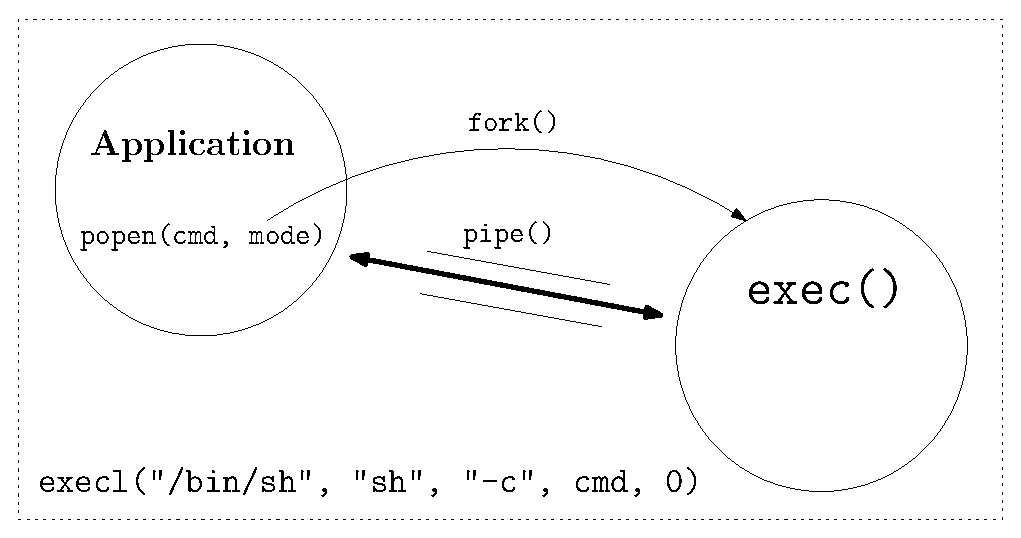
\includegraphics[width=90mm]{img/adv-ipc-and-io/popen.eps}
\end{center}


\begin{itemize}
\item As you can see from the picture, \texttt{popen()} can be used both to read
from and write data to the command. However, reading is probably the most common
case. And while it explicitly says ,,\texttt{fork}'', it does not have to be
like that, of course. The implementation is system depended because the UNIX
specification does not care about the actual implementation.
\item Creating a pipe, forking a new process, closing and redirecting some
descriptors -- all that is managed by the \texttt{popen()} call.
\item \texttt{FILE *popen(const char *command, const char *mode);}\\
\texttt{int pclose(FILE *stream);}
\end{itemize}

%===============================================================================
\subsection{\texttt{popen()} and \texttt{pclose()} example code}

\begin{lstlisting}
    /* Echo the output of "ls" command to my standard
     * output. */
    FILE *ptr;
    char *cmd = "/usr/bin/ls -d *";

    if ((ptr = popen(cmd, "r")) != NULL) {
            while (fgets(buf, BUFLEN, ptr) != NULL)
                    printf("%s", buf);
    } else
            err(1, "popen");

    pclose(ptr);
\end{lstlisting}

\begin{itemize}
\item We silently assume in the code that you know how to work with a FILE type.
This was not in the [\myun\myix-prog-I] lecture. See man page for
\texttt{fopen()} and \texttt{fclose()} if needed.
\item If you use threads, you should use \texttt{popen}/\texttt{pclose} instead
of thread unsafe \texttt{system(3c)}.
\item \priklad{adv-ipc-and-io/popen.c}
\item \emsl{Exercise:} modify the code so that you feed your standard input
through:\\ \texttt{tr [[:alpha:]] [[:upper:]]} using \texttt{popen()}. Print the
output of \texttt{tr} on the standard output of your program.
\end{itemize}

%===============================================================================
\subsection{Mechanisms for Creating a Process}

We know functions that somehow create a process for us:

\begin{itemize}
\item \texttt{fork(void)}
\item \texttt{fork\_all(void)}
	\begin{itemize}
	\item forks and duplicates all existing threads. That was the former
	default behaviour of Solaris threads, \texttt{fork\_all()} now exists
	to allow backward compatibility.
	\end{itemize}
\item \texttt{popen(const char *command, const char *mode)}
\item \texttt{system(const char *string)}
\end{itemize}

Now we add a new one:
\begin{itemize}
\item \texttt{posix\_spawn(...)}
\end{itemize}

\begin{itemize}
\item \texttt{fork\_all()} was already mentioned in [\myun\myix-prog-I].
\end{itemize}

%===============================================================================
\subsection{\texttt{posix\_spawn()}, \texttt{posix\_spawnp()}}

\begin{itemize}
\item creating a new process from a process image in a single step
	\begin{itemize}
	\item no need for a fork and exec in the program itself
	\item HW architectures w/o dynamic address translation can not easily
	provide \texttt{fork()} since the addresses in the process are physical
	addresses
	\end{itemize}
\item it is part of POSIX real time extensions (POSIX.1d), see [posix.1d]
\item note that there must be means to specify various attributes normally dealt
with after \texttt{fork()} but before \texttt{exec()}
	\begin{itemize}
	\item user/group ID changes, signal mask and file descriptor
	manipulations
	\end{itemize}
\end{itemize}

\begin{itemize}
\item See [\myun\myix-prog-I] for more info on the POSIX standards.
\end{itemize}

%===============================================================================
\subsection{Using \texttt{posix\_spawn()}}

\begin{tabbing}
int \funnm{posix\_spawn}(\=pid\_t *restrict \emph{pid},\\
		\>const char *restrict \emph{path},\\
		\>const posix\_spawn\_file\_actions\_t *\emph{file\_actions},\\
		\>const posix\_spawnattr\_t *restrict \emph{attrp},\\
		\>char *const \emph{argv}[restrict],\\
		\>char *const \emph{envp}[restrict]);
\end{tabbing}

\begin{itemize}
\item \texttt{posix\_spawnp()} function call is the same as
\texttt{posix\_spawn()} but \texttt{PATH} is used if the \texttt{path} argument
does not contain a slash
\item you need \texttt{path} and \texttt{argv}, everything else can be set to
\texttt{NULL}
\item however, to read from a pipe, for example, you will need to use \emph{file
actions}
\end{itemize}

\begin{itemize}
\item The \emph{pid} will be filled with the child's PID.
\item \emph{attrp} contains various attributes applied on the process like
user/group IDs, signal masks, process group membership, ...
\item File actions contains info on how to deal with individual file descriptors
(if needed). If \texttt{NULL}, the behaviour will be the same as with
\texttt{fork()}, including honoring the \texttt{FD\_CLOEXEC} flag.
\item \emph{argv} is mandatory, with at least \texttt{argv[0]} (+
\texttt{argv[1]} containing NULL).
\end{itemize}

%===============================================================================
\subsection{File actions}

\begin{itemize}
\item if you want to duplicate the standard output to a pipe in the child, for
example, you must use file actions
\end{itemize}

\begin{lstlisting}
posix_spawn_file_actions_t factions;

pipe(p);
flags = fcntl(p[0], F_GETFL);
/* FD_CLOEXEC works together with file actions. */
fcntl(p[0], F_SETFL, flags | FD_CLOEXEC);
posix_spawn_file_actions_init(&factions);
posix_spawn_file_actions_adddup2(&factions, p[1], 1);
posix_spawn_file_actions_addclose(&factions, p[1]));
\end{lstlisting}


\begin{itemize}
\item File actions are performed in the child in the order in which they were
added to the file action object. File actions are performed before file
descriptors tagged with the \texttt{FD\_CLOEXEC} flag are closed.
\item One more file action you can use is
\texttt{posix\_spawn\_file\_actions\_addclose}.
\item \priklad{adv-ipc-and-io/posix\_spawn.c}
\item \emsl{Exercise:} change the code so that the new process blocks
\texttt{SIGTERM} signal, then call ,,\texttt{sleep 99}'' from it, and then send
it a \texttt{SIGTERM} signal from the parent. After the parent exits check that
the child is stil alive, verifying that the mask has been set properly. You will
have to use the \texttt{attrp} argument of the \texttt{posix\_spawn()}.
\end{itemize}

%===============================================================================
\subsection{Solaris Event Ports}

\begin{itemize}
\item existing ``old'' event notification frameworks
	\begin{itemize}
	\item AIO
	\item timers
	\item \texttt{poll()} 
	\end{itemize}
\item no unified way to reap an application's completion of events in Solaris
before the event ports
\item all of these frameworks built independently
\item no unified mechanism to reap events
\item varying performance and scalability of the existing frameworks
\item \emsl{need for one common API}
\end{itemize}


\label{SOLARIS_EVENT_PORTS}

\begin{itemize}
\item Solaris event ports first appeared in Solaris 10.
\item Timers were not mentioned in [\myun\myix-prog-I] nor in this material. See
\texttt{set\-i\-timer()} and \texttt{clock\_gettime()} for more information.
\end{itemize}


%===============================================================================
\subsection{Solaris Event Ports (continuted)}

\begin{itemize}
\item the fundamental piece of the event completion framework is the \emph{port}
\item applications use ports to register and reap events on the objects of
interest

\begin{lstlisting}
/* Create a port. */
int portfd = port_create();

/* Register the events you are interested in. */
port_associate(portfd,  ... );

/* Block until an event appears on the port. */
port_get(portfd,  ... );
\end{lstlisting}
\end{itemize}


\label{SOLARIS_EVENT_PORTS}

\begin{itemize}
\item Solaris event ports first appeared in Solaris 10.
\item Source code example not provided yet. See manual pages for respective functions.
\item References:
	\begin{itemize}
	\item \url{http://developers.sun.com/solaris/articles/event\_completion.html}
	\item \url{http://blogs.oracle.com/dap/entry/event\_ports\_and\_performance}
	\item \url{http://blogs.oracle.com/barts/entry/entry\_2\_event\_ports}
	\end{itemize}
\end{itemize}

%    port_create(3C), port_get(3C), ...
%    http://blogs.oracle.com/barts/entry/entry_2_event_ports
%    http://blogs.oracle.com/dap/entry/event_ports_and_performance
%    event(3) (libevent)
%    port_associate(3c) ma informace o tom, jake jsou mozne eventy
%
%    http://blogs.oracle.com/praks/entry/file_events_notification
%
%  http://blogs.oracle.com/dap/entry/libevent_and_solaris_event_ports

%===============================================================================
\subsection{FreeBSD KQueue}

\begin{itemize}
\item Kqueue is another event notification interface
\item first appeared in FreeBSD 4.1
\item Kqueue enables the user to receive alerts regarding events on specified
targets very quickly
\item ported to NetBSD and OpenBSD
\end{itemize}


\begin{itemize}
\item See \texttt{kqueue(2)} manual page on FreeBSD for more information.
\item References:
	\begin{itemize}
	\item \url{http://people.freebsd.org/~jlemon/papers/kqueue.pdf}
	\end{itemize}
\end{itemize}

%===============================================================================
\subsection{\texttt{libevent} -- a portable aproach to event notifications}

\begin{itemize}
\item asynchronous event notification software library
\item can use \texttt{/dev/poll}, Solaris event ports, kqueue,
\texttt{select()}, \texttt{poll()}, and \texttt{epoll(4)}
\item if you need an event notification framework on several different
platforms, \texttt{libevent} might be exactly what you are looking for
	\begin{itemize}
	\item should compile on Linux, *BSD, Solaris, Max OSX, and Windows
	\end{itemize}
\item written by Niels Provos
\end{itemize}


\label{LIBEVENT}

\begin{itemize}
\item \texttt{epoll(4)} is an I/O event notification facility in the Linux
kernel.
\item We already mentioned \texttt{/dev/poll} on p. \pageref{DEV_POLL}.
\item References:
	\begin{itemize}
	\item \url{http://www.monkey.org/~provos/libevent}
	\item \url{http://blogs.oracle.com/dap/entry/libevent\_and\_solaris\_event\_ports}
	\end{itemize}
\end{itemize}

\endinput

%===============================================================================
% Secure Programming.
%===============================================================================

\section{Secure Programming}

\begin{itemize}
  \item Motivation/goal:
  \begin{itemize}
    \item learn from the mistakes of others
    \item know how to write secure code (approach, techniques)
    \item be aware of what could go wrong/sensitive areas
  \end{itemize}
  \item We are not dealing with:
  \begin{itemize}
    \item secure use of cryptography primitives
    \item side-channel attacks
    \item robust secure network protocol design
    \item exploit techniques and analysis \texttt{(1)}
  \end{itemize}
\end{itemize}


\begin{itemize}
  \item[(1)] while technically interesting topic (e.g. for more in depth
  understanding of call procedures, assembly, HW architecture and internals
  in general) this is certainly out of scope and not in line with the main
  goal of this chapter
\end{itemize}

%===============================================================================

\subsection{More secure programs}

\begin{itemize}
  \item Prevention: 
  \begin{itemize}
    \item use of secure functions (strlcpy/strlcat)
  \end{itemize}
  \item Making attacker's life harder
  \begin{itemize}
    \item random allocations (mmap, malloc, ld.so)
    \item protection of memory segments (non-executable stack) (1)
  \end{itemize}
  \item Impact minimization
  \begin{itemize}
    \item privilege revocation (ping)
    \item privilege separation (OpenSSH)
    \item isolation (chroot, systrace, virtualization)
    \item separate uids for each service (\texttt{\_ntp}, \texttt{\_snmpd}, ...)
    \item buffer overflow detection and reaction (canary in the stack)
  \end{itemize}
\end{itemize}


\begin{itemize}
\item[(1)] non-exec stack can be worked around by e.g. overwriting return
address pointer with address of \texttt{system()} routine in libc and
constructing a frame which contains \texttt{"/bin/sh"} as an argument.
\end{itemize}

%===============================================================================

\subsection{Generic rules}

\begin{itemize}
  \item Check input data thoroughly (and do the right thing if they do not fit)
  \item {\it Do not assume} (1) (but rather check to confirm)
  \item Focus on corner cases (and go through all of them in detail)
  \begin{itemize}
    \item this includes handling failures properly (2)
  \end{itemize}
\end{itemize}


\begin{itemize}
  \item[(1)] A quotation from a whiteboard in office of an engineer.
  \item[(2)] I.e. returning failure code all the way up, freeing unneeded
    resources and reacting on it
    \begin{itemize}
    \item e.g. memory leak in error path can lead to Denial Of Service (DoS) by
      injecting number of invalid requests. See CR XXX (n2cp leak).
    \end{itemize}
\end{itemize}

{\bf Task}:
\begin{enumerate}
  \item Intro: KSSL is in-kernel SSL proxy in OpenSolaris/Solaris. It had a
    interoperability bug related to SSL/TLS protocol implementation.
  \item problem statement: {\it "... we needlessly fail a client hello request
        that has other compression methods in addition to the mandatory null
        compression method. This should be allowed since the spec allows
        supporting only the mandatory CompressionMethod.null and ignoring
        any other methods in client hello."}
  \item see the webrev \texttt{XXX/client\_hello.webrev.1} with
    the proposed fix
    \begin{itemize}
    \item focus on \texttt{kssl\_handle\_client\_hello()}
    \end{itemize}
  \item input info:
     \begin{itemize}
     \item m-block structure (\texttt{mblk\_t *mp}) represents SSL Client
     Hello message
     \item \texttt{mp->b\_rptr} is the beginning (pointer to area where we
     can start reading), \texttt{b\_wptr} is the end (pointer to area
     where we can start writing)
     \item see the definition in \texttt{usr/src/uts/common/sys/stream.h}:
\begin{verbatim}
    363 /*
    364  * Message block descriptor
    365  */
    366 typedef struct	msgb {
    367 	struct	msgb	*b_next;
    368 	struct  msgb	*b_prev;
    369 	struct	msgb	*b_cont;
    370 	unsigned char	*b_rptr;
    371 	unsigned char	*b_wptr;
    372 	struct datab 	*b_datap;
    373 	unsigned char	b_band;
    374 	unsigned char	b_tag;
    375 	unsigned short	b_flag;
    376 	queue_t		*b_queue;	/* for sync queues */
    377 } mblk_t;
\end{verbatim}
  \end{itemize}
   \item the assignment:
   \begin{enumerate}
        \item find the problem with the proposed fix
        \begin{itemize}
          \item hint: it's handy to look into the TLSv1 spec RFC 2246
                  (sections 4.3, 7.4.1.2)
          \item use code review/inspection approach (reader role)
	  \item What would happen if someone exploited the problem ?
	    (see first point of this Task)
        \end{itemize}
	\item once the problem is clear, propose correct solution
          \begin{itemize}
	  \item compare your solution with \texttt{XXX/client\_hello.webrev.2}
          \end{itemize}
   \end{enumerate}
\end{enumerate}

%===============================================================================

\subsection{Checking where necessary}

\begin{itemize}
  \item checking return values is not only useful for graceful handling of
    errors but can also have security impact
  \item assuming a function does always the right thing can later undermine
    sensitive area of code
\end{itemize}


{\bf Example}: \texttt{rtld} local root exploit in FreeBSD 7.2
\begin{itemize}
  \item intro: in FreeBSD, when loading setuid/setgid programs into memory,
                  dynamic (run-time) loader scrubs the environment so it
		  does not contain insecure (read user supplied) variables.
		  (mainly \texttt{LD\_LIBRARY\_PATH} and \texttt{LD\_PRELOAD})
   \begin{itemize}
   \item this is done via \texttt{unsetenv()} defined in
     \url{http://www.freebsd.org/cgi/cvsweb.cgi/src/lib/libc/stdlib/getenv.c:unsetenv()}
   \end{itemize}
  \item see the code in:
        \url{http://www.freebsd.org/cgi/cvsweb.cgi/src/libexec/rtld-elf/rtld.c}
    \begin{itemize}
    \item function \texttt{\_rtld()} is the "main entry point for dynamic
       linking". It contains this section:
    \end{itemize}
\begin{verbatim}
    trust = !issetugid();

    ld_bind_now = getenv(LD_ "BIND_NOW");
    /* 
     * If the process is tainted, then we un-set the dangerous environment
     * variables.  The process will be marked as tainted until setuid(2)
     * is called.  If any child process calls setuid(2) we do not want any
     * future processes to honor the potentially un-safe variables.
     */
    if (!trust) {
        unsetenv(LD_ "PRELOAD");
        unsetenv(LD_ "LIBMAP");
        unsetenv(LD_ "LIBRARY_PATH");
        unsetenv(LD_ "LIBMAP_DISABLE");
        unsetenv(LD_ "DEBUG");
        unsetenv(LD_ "ELF_HINTS_PATH");
    }
\end{verbatim}
  \item let's look at GETENV(3) man page which describes the semantics of
    return values of \texttt{unsetenv()}:
\begin{verbatim}
     The unsetenv() function deletes all instances of the variable name
     pointed to by name from the list.

RETURN VALUES
...
     The setenv(), putenv(), and unsetenv() functions return the value 0 if
     successful; otherwise the value -1 is returned and the global variable
     errno is set to indicate the error.

     [EINVAL]           The function getenv(), setenv() or unsetenv() failed
                        because the name is a NULL pointer, points to an empty
                        string, or points to a string containing an ``=''
                        character.
...
     [EFAULT]           The functions setenv(), unsetenv() or putenv() failed
                        to make a valid copy of the environment due to the
                        environment being corrupt (i.e., a name without a
                        value).  A warning will be output to stderr with
                        information about the issue.
\end{verbatim}
    \item the first case is no-variable/no-value, the latter is
    variable/no-value.
\begin{verbatim}
/*
 * Unset variable with the same name by flagging it as inactive.  No variable is
 * ever freed.
 */
int
unsetenv(const char *name)
{
        int envNdx;
        size_t nameLen;

        /* Check for malformed name. */
        if (name == NULL || (nameLen = __strleneq(name)) == 0) {
                errno = EINVAL;
                return (-1);
        }

        /* Initialize environment. */
        if (__merge_environ() == -1 || (envVars == NULL && __build_env() == -1))
                return (-1);

        /* Deactivate specified variable. */
        envNdx = envVarsTotal - 1;
        if (__findenv(name, nameLen, &envNdx, true) != NULL) {
                envVars[envNdx].active = false;
                if (envVars[envNdx].putenv)
                        __remove_putenv(envNdx);
                __rebuild_environ(envActive - 1);
        }

        return (0);
}
\end{verbatim}
  \item it calls \texttt{\_\_merge\_environ()} which contains this code:
\begin{verbatim}
          if (origEnviron != NULL)
                for (env = origEnviron; *env != NULL; env++) {
                        if ((equals = strchr(*env, '=')) == NULL) {
                                __env_warnx(CorruptEnvValueMsg, *env,
                                    strlen(*env));
                                errno = EFAULT;
                                return (-1);
                        }
\end{verbatim}
	  \item the \texttt{*envp[]} array contains pointers to strings like:
	    \texttt{HOME=/home/user} , \texttt{TERM=xterm} and such
	    \begin{itemize}
	    \item so if we replace one of the env strings by value-less string
	      \texttt{unsetenv()} will bail out as above and will not unset the
	      variable
	    \end{itemize}
  \item compare the above with OpenSolaris approach of handling setuid/setgid
	    programs:
\url{http://src.opensolaris.org/source/xref/onnv/onnv-gate/usr/src/cmd/sgs/rtld/common/setup.c:setup()}
  \begin{itemize}
   \item \texttt{setup()} which contains the main rtld functionality calls
   \texttt{security()} which performs the setuid/setgid check:
\begin{verbatim}
     	/*
     	 * Determine whether we have a secure executable.
     	 */
     	security(uid, euid, gid, egid, auxflags);
\end{verbatim}
  \item \texttt{security()} defined in
\url{http://src.opensolaris.org/source/xref/onnv/onnv-gate/usr/src/cmd/sgs/rtld/common/util.c#security}
  only sets the per-process \texttt{RT\_FL\_SECURE} flag
  (lines 3464, 3474, 3481).
\begin{verbatim}
   3445 /*
   3446  * Determine whether we have a secure executable.  Uid and gid information
   3447  * can be passed to us via the aux vector, however if these values are -1
   3448  * then use the appropriate system call to obtain them.
   3449  *
   3450  *  -	If the user is the root they can do anything
   3451  *
   3452  *  -	If the real and effective uid's don't match, or the real and
   3453  *	effective gid's don't match then this is determined to be a `secure'
   3454  *	application.
   3455  *
   3456  * This function is called prior to any dependency processing (see _setup.c).
   3457  * Any secure setting will remain in effect for the life of the process.
   3458  */
   3459 void
   3460 security(uid_t uid, uid_t euid, gid_t gid, gid_t egid, int auxflags)
   3461 {
   3462         if (auxflags != -1) {
   3463                 if ((auxflags & AF_SUN_SETUGID) != 0)
   3464                         rtld_flags |= RT_FL_SECURE;
   3465                 return;
   3466         }
   3467 
   3468         if (uid == (uid_t)-1)
   3469                 uid = getuid();
   3470         if (uid) {
   3471                 if (euid == (uid_t)-1)
   3472                         euid = geteuid();
   3473                 if (uid != euid)
   3474                         rtld_flags |= RT_FL_SECURE;
   3475                 else {
   3476                         if (gid == (gid_t)-1)
   3477                                 gid = getgid();
   3478                         if (egid == (gid_t)-1)
   3479                                 egid = getegid();
   3480                         if (gid != egid)
   3481                                 rtld_flags |= RT_FL_SECURE;
   3482                 }
   3483         }
   3484 }
\end{verbatim}
  \item \texttt{LD\_PRELOAD} handling is done in \texttt{ld\_preload()}
  defined in
\url{http://src.opensolaris.org/source/xref/onnv/onnv-gate/usr/src/cmd/sgs/rtld/common/setup.c#ld\_preload}:
\begin{verbatim}
         /*
          * If this a secure application, then preload errors are
          * reduced to warnings, as the errors are non-fatal.
          */
         if (rtld_flags & RT_FL_SECURE)
                 rtld_flags2 |= RT_FL2_FTL2WARN;
         if (expand_paths(*clmp, ptr, &palp, AL_CNT_NEEDED,
             PD_FLG_EXTLOAD, 0) != 0)
\end{verbatim}
  \item \texttt{expand\_paths()} defined in
  \url{http://src.opensolaris.org/source/xref/onnv/onnv-gate/usr/src/cmd/sgs/rtld/common/paths.c#expand\_paths}
  contains the actual check:
\begin{verbatim}
          /*
           * If this a secure application, validation of the expanded
           * path name may be necessary.
           */
          if ((rtld_flags & RT_FL_SECURE) &&
              (is_path_secure(str, clmp, orig, tkns) == 0))
          	continue;
\end{verbatim}
      \begin{itemize}
	\item this is different approach (set flag and check where needed)
	  which allows bigger flexibility. (but the checks have to be in
	  the right places as opposed to scrub-before-doing-anything
	  approach used in FreeBSD)
	  \begin{itemize}
	  \item ld.so.1(1) SECURITY section has more details, section FILES
	    sums it up:
    \texttt{/lib/secure} and \texttt{/usr/lib/secure} are
         \texttt{LD\_PRELOAD} locations for secure applications.
    \texttt{/lib/secure/64} and \texttt{/usr/lib/secure/64} are
         \texttt{LD\_PRELOAD} locations for secure 64-bit applications.
	 \item the locations are empty by default and writable only by
	 \texttt{root}.
	 \end{itemize}
     \end{itemize}
    \end{itemize}
  \item References:
    \begin{itemize}
    \item \url{http://xorl.wordpress.com/2009/12/01/freebsd-ld\_preload-security-bypass/}
    \item \url{http://stealth.openwall.net/xSports/fbsd-rtld-full-package}
    \end{itemize}
\end{itemize}

%===============================================================================

\subsection{Function classification}

\begin{itemize}
\item Library functions can be divided into several equivalence classes
  according to how secure/usable they are
    \begin{itemize}
    \item Some functions are inherently insecure and cannot be safely used
      at all
    \item Other functions require great deal of attention to get the code
      right (correct+secure code)
    \item There are even some functions which offer consistent API/behavior
      and make it easier to work with corner cases
    \end{itemize}
\end{itemize}


\begin{itemize}
  \item categorized list of functions:
    \url{http://hub.opensolaris.org/bin/view/Community+Group+security/funclist}
  \item Secure programming guidance at OpenSolaris Security community
    \url{http://www.opensolaris.org/os/community/security/library/secprog}
  \item Secure programming presentation by Scott Rotondo
    \url{http://opensolaris.org/os/community/security/library/secprog/secure\_prog.pdf}
\end{itemize}

%===============================================================================

\subsection{Buffer overflows}

\begin{itemize}
  \item informal definition: writing past the end of a buffer
  \begin{itemize}
    \item comon cases:
    \begin{itemize}
      \item string buffers but can be any buffer space
      \item buffer on the stack but applies also for on the heap buffers
    \end{itemize}
  \end{itemize}
  \item the danger:
  \begin{itemize}
    \item the surroundings of the buffer being overflowed (stack)
    \begin{itemize}
      \item function return address (redirecting code flow) \texttt{(1)}
      \item frame pointer (altering code flow)
    \end{itemize}
  \item persistent system space (heap)
    \begin{itemize}
      \item FILE I/O space
    \end{itemize}
  \end{itemize}
\end{itemize}


\begin{itemize}
  \item What happens on overflow:

\begin{verbatim}
  high address -------------------
                 heap
               -------------------


               -------------------
                return address
               -------------------
                frame pointer
               -------------------

                local variables

               -------------------

                       |
                       | stack grows downwards
                       v


  low address --------------------
\end{verbatim}
  \item[(1)] Smashing The Stack For Fun And Profit, Phrack Volume Seven, Issue
  49: \url{http://www.phrack.com/issues.html?issue=49\&id=14\&mode=txt}
\end{itemize}

%===============================================================================

\subsection{Safe string manipulation 1/2}

\begin{itemize}
  \item no boundary check: gets(), strcpy(), strcat(), sprintf()/vsprintf() (1)
  \item watch out when using: strncpy()/strncat()
\end{itemize}


\begin{itemize}
\item[(1)] unsafe functions:
  \begin{itemize}
  \item gets() does not check boundaries at all
  \end{itemize}
\item potentionally unsafe / avoid:
  \begin{itemize}
  \item strcpy(), strcat()
    \begin{itemize}
    \item do not check boundaries at all
    \item strcpy() does not zero terminate on overflow (but strcat() does)
    \item possible to calculate the necessary dst size for strcat()
      but hard to follow the code
    \end{itemize}
  \item sprintf()/vsprintf()
    \begin{itemize}
    \item no boundary check
    \item possible approach: compute the buffer size + control the fmt string
    \end{itemize}
  \end{itemize}
\item potentionally unsafe / use with caution:
  \begin{itemize}
  \item scanf() family
    \item scanf() should not be called without limit
      \item \texttt{scanf("\%s", str);} is asking for buffer overflow
      \item \texttt{scanf("\%10s", str);} needs 11 characters buffer
         (+ terminating \texttt{'\\\\0'})
  \end{itemize}
  \item snprintf()/vsnprintf()
  \begin{itemize}
    \item return the number of characters necessary (without the zero), not the
      actual number of characters written to the buffer
      - watch out for constructions like this:
        p += snprintf(p, lenp, "...");
  \end{itemize}
  \item strncpy()
  \begin{itemize}
    \item does not zero terminate on overflow
    \item zero-fills the remainder of the dst buffer in no-overflow case (perf)
  \end{itemize}
  \item strncat()
  \begin{itemize}
    \item always terminates (even on overflow)
    \item is not intuitive - some arithmetics for the size argument is almost
      always needed
  \end{itemize}
\end{itemize}


%===============================================================================

\subsection{Safe string manipulation 2/2}

\begin{itemize}
  \item overflow aware+helping: string(3C): \\
    \texttt{size\_t \funnm{strlcpy}(char *\emph{dst}, const char
    *\emph{src}, size\_t \emph{dstsize});} \\
    \texttt{size\_t \funnm{strlcat}(char *\emph{dst}, const char
    *\emph{src}, size\_t \emph{dstsize});}
  \begin{itemize}
    \item always terminate with zero, even in case of buffer overflow
    \item do not zero-out the rest of the dst string
    \item easy truncation detection
    \item the \emph{dstsize} argument is the total space in \emph{dst}
    \item for \texttt{strlcat()} nothing happens if the dst string is longer
      than size
    \item \texttt{strlcat()} returns
      \texttt{min\{dstsize,strlen(dst)\}+strlen(src)}
  \end{itemize}
\end{itemize}


\begin{itemize}
  \item[(1)] unfortunately, \texttt{strlcpy()}/\texttt{strlcat()} are not
  available in Linux world
    \begin{itemize}
    \item the main reasons for rejection (for inclusion into GNU libc) seem
      to be:
      \begin{enumerate}
      \item the functions are non-standard
      \item risk of truncation is considered to be greater than risk of overflow
      \end{enumerate}
    \end{itemize}
    \item the exact reasons are not very clear because of the strong language
      used by RedHat developers who are opposing the idea:
    \begin{itemize}
      \item \url{http://sources.redhat.com/ml/libc-alpha/2000-08/msg00061.html}
      \item \url{http://sources.redhat.com/ml/libc-alpha/2000-08/msg00053.html}
        (links from \url{http://en.wikipedia.org/wiki/Strlcpy\#Criticism})
    \end{itemize}
    \item that's why the Task below is even more important when writing
      code which uses static arrays because to make the code work on Linux
      as well there are basically 2 choices:
      \begin{itemize}
        \item either use the unsecure/inconsistent functions (not recommended)
	\item attach strlcpy/strlcat implementation (just like many projects do)
      \end{itemize}
\end{itemize}

\begin{itemize}
\item ensuring zero termination with \texttt{strncpy()/strncat()}:
  \begin{itemize}
  \item pass \texttt{dstlen - 1} as length and terminate by hand:
    \begin{verbatim}
    dst[dstlen] = '\0';
    \end{verbatim}
    \begin{itemize}
    \item if the dst variable is static or \texttt{calloc()}'ed the zero
      termination is not necessary but the code is then harder to inspect
      for overflow problems
    \end{itemize}
  \end{itemize}
\item problems with using \texttt{strncat()}:
  \begin{itemize}
  \item the size passed is the free space available in the buffer (not the
    total size of the buffer)
  \item the size argument must not count the terminating zero
    (even though the function always terminates)
  \end{itemize}
\item check for buffer overflow/truncation:
\begin{verbatim}
       if (strlcpy(dst, src, dstsize) >= dstsize)
               return (-1);

       if (snprintf(buf, sizeof (buf), "%s", src) >= sizeof (buf))
		return (-1);
\end{verbatim}
  \begin{itemize}
  \item the 'equal' case is where the string fits but without the
     terminating zero
  \end{itemize}
  \item \texttt{strlcpy()} paper:
    \url{http://www.openbsd.org/papers/strlcpy-paper.ps}
\end{itemize}

{\bf Task}: Write a secure (detects and prevents buffer overflow) function 
          \funnm{foo()} which constructs a string using the
          folllowing rule. The size of
	  the destination string is passed to the function.
	  Use hard-coded value in the \texttt{main()} calling \funnm{foo()}
	  (use e.g. \texttt{MAXPATHLEN} def{}ine from \texttt{<sys/param.h>}).

          \begin{itemize}
	  \item prototype: \texttt{int \funnm{foo}(char *\emph{input},
	    char *\emph{dst}, size\_t \emph{dstlen});}
	  \item rule (+ means concatenation):
          \begin{verbatim}
            env("HOME") + "/" + argv[1] + "/.foorc"
          \end{verbatim}
            \begin{itemize}
	    \item which means \texttt{main()} will pass \texttt{argv[1]}
	    to \funnm{foo()} as \emph{input}.
            \end{itemize}
 	  \item write using:
          \begin{enumerate}
	    \item \texttt{strcpy()}/\texttt{strcat()} (optional, only for
	      the really patient)
            \item \texttt{strncpy()}/\texttt{strncat()}
            \item \texttt{strlcpy()}/\texttt{strlcat()}
          \end{enumerate}
	  \item The function should return the length of the string or
             in case of overflow a negative number which if placed in
	     \texttt{abs()} is equal to the number of missing characters
	     in the destination string.
	  \item Construct number of unit tests for all possible cases
	    (most importantly for corner cases) and verify that each of the
	    implementations works correctly.
          \end{itemize}


%===============================================================================

\subsection{Time of use versus time of check}

\begin{itemize}
  \item possible race conditions - a window between check and use
    where the actual object can be swapped/changed but the reference to
    the object remains the same.
  \item setuid/setgid program often needs to verify that once it switches
    to a user the user will be able to read a file
  \item access(2) does the check using real uid/gid
\end{itemize}


\begin{itemize}
  \item Example of insecure approach (assume \texttt{path} points to a
  file in directory writable by others):
\begin{verbatim}
    /* we're running with euid = 0, and ruid = userid != 0 */
    if (access(path, R_OK|W_OK) < 0)
            return -1;

    fd = open(path, O_RDWR);
    ...
\end{verbatim}
  \begin{itemize}
  \item access(2) resolves the path to a XXX and performs the check. After
    that the XXX object is free'd. open(2) does the lookup again XXX.
    Problem is that this time different object can be used - the operation
    of check and return is not atomic. Now the setuid application might be
    writing to different file.
  \item correct approach: switch to the user and try to open the file -> no
    race condition
\begin{verbatim}
  seteuid(getuid());
  if ((fd = open(path, O_RDWR)) == -1)
      err(1, "open")
  seteuid(0);
\end{verbatim}
  \end{itemize}
  \item similar problem with stat():
\begin{verbatim}
  /* make sure "path" is a regular file before opening */
  if (stat(path, &buf) == -1 || !S_ISREG(buf.st_mode))
     err(...);
  fd = open(path, O_RDONLY);
\end{verbatim}
  \begin{itemize}
  \item the solution:
\begin{verbatim}
  if ((fd = open(path, O_NONBLOCK|O_RDONLY)) == -1)
     err(...);
  if (fstat(fd, &buf) == -1 || !S_ISREG(buf.st_mode))
     err(...);
\end{verbatim}
  \end{itemize}
  \begin{itemize}
  \item \texttt{O\_NONBLOCK} will prevent blocking when opening a device
  \end{itemize}
\item other functions which take file descriptor as argument instead of
  filename: \texttt{fchmod()} (chmod(2)), \texttt{fchdir()} (chdir(2)),
            \texttt{fchroot()} (chroot(2)), ...
\end{itemize}


%===============================================================================

\subsection{Memory locking}

\begin{itemize}
  \item prevents a memory region from being swapped out to disk (1)
  \item mlock() is perfectly useful for password managers, for example
  \item it seems one must use mmap() on Solaris to ensure the correct
    memory alignment (2)
  \item plock() is more generic but less granular
    \begin{itemize}
      \item allows locking of text/data segments
    \end{itemize}
  \item mlockall() locks every current/future mapped page in the address space
    \begin{itemize}
      \item the same semantics as mlock()
      \item can do selective unlock with munlock()
    \end{itemize}
\end{itemize}


\begin{itemize}
\item[(1)] semantics:
  \begin{itemize}
  \item no fork() inheritance
    \begin{itemize}
    \item unless \texttt{MAP\_PRIVATE} mmap() flag is used
    \end{itemize}
  \item locking of the same page by multiple processes is reference counted
    \begin{itemize}
    \item the last process which unlocks results in the page being unlocked
    \end{itemize}
  \item single process locking of the same page is not nested
    \begin{itemize}
    \item i.e. single unlock of page locked multiple times does unlock
    \end{itemize}
  \end{itemize}
  \item[(2)] see \priklad{secure-prog/mlock.c}
\end{itemize}

%===============================================================================

\subsection{Temporary files handling}

\begin{itemize}
\item mktemp(3C): \texttt{char *\funnm{mktemp}(char *\emph{template})}
  \begin{itemize}
    \item should not be used because of race condition between check and create
  \end{itemize}
\item mkstemp(3C)/mkdtemp(3C):
  \texttt{int \funnm{mkstemp}(char *\emph{template})}
  \begin{itemize}
  \item secure, race condition-less variants - return file descriptor of the
      temporary file and replaces the template argument with filename
  \end{itemize}
\item XXX following symlinks
\end{itemize}


Example: mktemp(1) in shell script

\begin{verbatim}
TMPFILE=`mktemp /tmp/example.XXXXXX`
if [[ -z "$TMPFILE" ]]; then exit 1; fi
print "program output" >> $TMPFILE
\end{verbatim}

%===============================================================================

\subsection{Off-by-one errors / Integer overflows}

\begin{itemize}
\item \texttt{calloc()} can overflow internally (1)
\item XXX off-by-one
\end{itemize}


\begin{itemize}
  \item[(1)] when computing the size of the number of bytes to be
  allocated XXX
\end{itemize}


%===============================================================================

\subsection{Format string overflows}

\begin{itemize}
\item XXX user-supplied format string can be used to overflow stack of the
process
  - examples XXX:
    %n
    %x
\end{itemize}



%===============================================================================

\subsection{Privilege separation}

\begin{itemize}
  \item the goal: minimize the amount of code running as root/with privileges
  \item basic principle - one unprivileged process for input data processing,
		    another process for performing privileged tasks.
		    they communicate with each other using set of well
                    defined messages.
\end{itemize}


XXX picture


%===============================================================================

\subsection{Examples of privilege separated programs}

\begin{itemize}
\item OpenSSH:
  \begin{itemize}
  \item master process: accepts new connections, then immediately forks new
    process group (1)
  \item alternative privilege separation model (2)
  \end{itemize}
\item OpenBGPD
  \begin{itemize}
  \item parent: runs as root, enters routes into kernel
    - works with routing socket (3)
  \end{itemize}
\item OpenNTPD
  \begin{itemize}
  \item parent: runs as root, sets the time
  \item ntp engine: runs as non-root uid/gid \texttt{\_ntp:\_ntp} and
     chrooted to \texttt{/var/empty}
  \item simple communication (4)
  \end{itemize}
\end{itemize}


\begin{itemize}
  \item[(1)] process group consists of:
    \begin{itemize}
     \item monitor: privileged process, handles authentication
     \item listener: SSH communication over the network
    \end{itemize}
  \item[(2)] OpenSSH: XXX privsep protocol with XXX messages
    - SunSSH: altprivsep with XXX messages
  \item[(3)] children processes:
    \begin{itemize}
    \item child \#1 (session engine): manages sessions (TCP connections)
    - runs as unprivileged user \texttt{\_bgpd}, chroots to \texttt{/var/empty}
    \item child \#2 (route decision engine): works with routing tables
    - runs as unprivileged user \texttt{\_bgpd}, chroots to \texttt{/var/empty}
    \end{itemize}
  \item[(4)] \texttt{socketpair}, 2 message types (set the time, lookup
     hosts using the files in \texttt{/etc})
\end{itemize}

%===============================================================================

\subsection{Privilege revocation/bracketting}

\begin{itemize}
  \item use only the privileges which are needed (at the time they are needed)
  \item \texttt{seteuid()}
    \begin{itemize}
      \item better: \texttt{setreuid(getuid(), getuid());}
    \end{itemize}
  \item privilege awareness (privileges(5) on Solaris)
\end{itemize}



%===============================================================================

\subsection{Non-executable stack}

\begin{itemize}
\item XXX
\item XXX OpenBSD approach for platforms lacking N-X
\end{itemize}

\texttt{cc -M /usr/lib/ld/map.noexstk myprogram.c}



%===============================================================================

\subsection{Prevention techniques and tools}

\begin{itemize}
\item check return values of functions (and interpret + act upon them correctly)
  \begin{itemize}
    \item use \texttt{-Wall} and fix all warnings
  \end{itemize}
\item chroot(2) syscall
  \begin{itemize}
  \item close unneeded descriptors \bf{and} \texttt{chdir()} \bf{and}
   \texttt{chroot()}
  \end{itemize}
\item automated checking
  \begin{itemize}
  \item lint, Parfait, XXX
  \end{itemize}
\item stress testing (1)
\item peer code reviews
\item do the what-went-wrong case studies regularly (2)
\end{itemize}


\begin{itemize}
  \item[(1)] try to break the program (e.g. by feeding it all sorts of bogus
   data, injecting faults, etc.)
  \item[(2)] Analyses of vulnerabilities/fixes: \url{http://xorl.wordpress.com}
    (be sure to double check/do your research, though)
  \item References:
  \begin{itemize}
    \item CERT C secure coding standard:
      \url{https://www.securecoding.cert.org/}
    \item Secure Coding in C and C++ (Robert C. Seacord)
      \url{http://www.cert.org/books/secure-coding/}
  \end{itemize}
\end{itemize}

\endinput

%===============================================================================
% Changelog.
%===============================================================================

\newpage

\emsl{ChangeLog} 

\label{CHANGELOG}

% empty para
~

{\footnotesize
\begin{itemize}
\item[{\bfseries 2016-03-10}] Removal of some OS specific sections from
,,Debugging'' section
\item[{\bfseries 2016-03-08}] Minor changes to testing, start using new tasks
formatting.
\item[{\bfseries 2016-03-04}] Overhaul of the formatting and style.
\item[{\bfseries 2010-10-25}] More information on a difference between Bash and
the Korn shell, p\pageref{BASH_KSH}.
\item[{\bfseries 2010-05-11}] More info on the \texttt{SIGHUP} signal, p.
\pageref{SIGHUP_SIGNAL}.
\item[{\bfseries 2010-02-18}] Some fixes in the terminal chapter.
\item[{\bfseries 2009-12-30}] Bulk of changes for the ,,Secure programming'' and
,,Advanced networking'' chapters.
\item[{\bfseries 2010-01-03}] Thread chapter.
\item[{\bfseries 2009-11-29}] More work on the ,,Advanced IPC and IO'' chapter.
\item[{\bfseries 2009-11-21}] ,,Terminals'' chapter more or less ready, initial
,,Advanced IPC and IO'' section. It looks that the ,,Debugging'' chapter is also
quite ready.
\item[{\bfseries 2009-11-10}] better ,,Testing'' section, initial ,,Debugging''
chapter.
\item[{\bfseries 2009-08-30}] 1st version of this material compiled.
\end{itemize}
}

\newpage

\endinput


\end{document}
